%-------------------------------------------------------------------------------
%                      Template Naskah Skripsi
%               	Berdasarkan format JTETI FT UGM
% 						(c) @gunturdputra 2014
%-------------------------------------------------------------------------------

%Template pembuatan naskah skripsi.
\documentclass{jtetiskripsi}

%Untuk prefiks pada daftar gambar dan tabel
\usepackage[titles]{tocloft}
\renewcommand\cftfigpresnum{Gambar\  }
\renewcommand\cfttabpresnum{Tabel\   }

%Untuk hyperlink dan table of content
\usepackage[hidelinks]{hyperref}
\newlength{\mylenf}
\settowidth{\mylenf}{\cftfigpresnum}
\setlength{\cftfignumwidth}{\dimexpr\mylenf+2em}
\setlength{\cfttabnumwidth}{\dimexpr\mylenf+2em}

%Untuk Bold Face pada Keterangan Gambar
\usepackage[labelfont=bf]{caption}

%Untuk caption dan subcaption
\usepackage{caption}
\usepackage{subcaption}
\usepackage{xspace}


%pdf
\usepackage{pdfpages}

%table
\usepackage{array}
\usepackage{longtable}
\newcolumntype{P}[1]{>{\centering\arraybackslash}p{#1}}
\usepackage{graphics}
\usepackage{wrapfig}

%bibliography
\usepackage[
  style=authoryear-icomp,
  maxcitenames=1,
  isbn=false,
  backend=biber,
  doi=false,
  url=false,
  autolang=other,
  hyperref=true,
  sortcites=true,
  bibwarn=true,
  firstinits=true,
  autolang=other,
]{biblatex}
\DefineBibliographyStrings{english}{%
  andothers = {et al\adddot,\addspace},
}
\renewcommand*{\nameyeardelim}{\addcomma\space}
\DeclareFieldFormat{citehyperref}{%
  \DeclareFieldAlias{bibhyperref}{noformat}% Avoid nested links
  \bibhyperref{#1}}

\DeclareFieldFormat{textcitehyperref}{%
  \DeclareFieldAlias{bibhyperref}{noformat}% Avoid nested links
  \bibhyperref{%
    #1%
    \ifbool{cbx:parens}
      {\bibcloseparen\global\boolfalse{cbx:parens}}
      {}}}

\savebibmacro{cite}
\savebibmacro{textcite}

\renewbibmacro*{cite}{%
  \printtext[citehyperref]{%
    \restorebibmacro{cite}%
    \usebibmacro{cite}}}

\renewbibmacro*{textcite}{%
  \ifboolexpr{
    ( not test {\iffieldundef{prenote}} and
      test {\ifnumequal{\value{citecount}}{1}} )
    or
    ( not test {\iffieldundef{postnote}} and
      test {\ifnumequal{\value{citecount}}{\value{citetotal}}} )
  }
    {\DeclareFieldAlias{textcitehyperref}{noformat}}
    {}%
  \printtext[textcitehyperref]{%
    \restorebibmacro{textcite}%
    \usebibmacro{textcite}}}
\addbibresource{daftar-pustaka.bib}

%equation
\usepackage{amsmath}

%algorithm & syntax
\usepackage{algorithm}
\usepackage{algpseudocode}
\usepackage{algorithmicx}
% \usepackage{algcompatible}
\algnewcommand\algorithmicforeach{\textbf{for each:}}
\algnewcommand\ForEach{\item[ \algorithmicforeach]}
\algdef{SE}[DOWHILE]{Do}{doWhile}{\algorithmicdo}[1]{\algorithmicwhile\ #1}%
\newenvironment{conditions}
  {\par\vspace{\abovedisplayskip}\noindent\begin{tabular}{>{$}l<{$} @{${}={}$} l}}
  {\end{tabular}\par\vspace{\belowdisplayskip}}

%code
\usepackage{listings}
\usepackage{xcolor}
\definecolor{codegreen}{rgb}{0,0.6,0}
\definecolor{codegray}{rgb}{0.5,0.5,0.5}
\definecolor{codepurple}{rgb}{0.58,0,0.82}
\lstdefinestyle{mystyle}{
    commentstyle=\color{codegreen},
    keywordstyle=\color{magenta},
    numberstyle=\tiny\color{codegray},
    stringstyle=\color{codepurple},
    basicstyle=\ttfamily\footnotesize,
    frame=single,
    breakatwhitespace=false,
    breaklines=true,
    captionpos=b,
    keepspaces=true,
    numbersep=5pt,
    showspaces=false,
    showstringspaces=false,
    showtabs=false,
    tabsize=2
}
\lstset{style=mystyle}
\makeatletter
\def\thechapter{\@Roman\c@chapter}
\AtBeginDocument{%
  \def\thelstlisting{\@arabic\c@chapter.\@arabic\c@lstlisting}}
\makeatother

%Create a new minipage environment where paragraphs have indents
\newlength{\currentparindent}
\newenvironment{minipageparindent}[2][c]
  {\setlength{\currentparindent}{\parindent}% save the value
   \noindent\begin{minipage}[#1]{#2}% open the minipage
   \setlength{\parindent}{\currentparindent}% restore the value
  }
  {\end{minipage}}

%Create an environment that creates a paragraph with a picture next to it, both being aligned at the top.
\newenvironment{pictureparagraph}[1]    %argument is an 'includegraphics' command
    {\newcommand\picturetoplace{#1}     % using variable directly gives an error
    \begin{minipageparindent}[t]{0.7\textwidth} %
    \vspace{0pt}    %Make sure that the top base is at the absolute top
    }   
    {
    \end{minipageparindent}
    \begin{minipage}[t]{0.3\textwidth}
    \vspace{0pt}    %Make sure that the top base is at the absolute top of the minipage
    \picturetoplace
    \end{minipage}\\}



%-----------------------------------------------------------------
%Disini awal masukan untuk data proposal skripsi
%-----------------------------------------------------------------
\titleind{DETEKSI AREA KELILING LUKA KRONIS DENGAN MENGGUNAKAN ALGORITMA \emph{GRABCUT}}

\fullname{Muhammad Hafiz Hisbullah}

\idnum{1313619019}

\approvaldate{11 Januari 2024}

\degree{Sarjana Ilmu Komputer}

\yearsubmit{2024}

\program{Ilmu Komputer}

\dept{Ilmu Komputer}

\firstsupervisor{Muhammad Eka Suryana, M. Kom.}
\firstnip{197706152003121001}

\secondsupervisor{Drs. Mulyono, M. Kom.}
\secondnip{196605171994031003}

%-----------------------------------------------------------------
%Disini akhir masukan untuk data proposal skripsi
%-----------------------------------------------------------------

\tolerance=1
\emergencystretch=\maxdimen{}
\hyphenpenalty=10000
\hbadness=10000

\begin{document}

\cover{}
\clearpage{}
\setcounter{page}{0}
%-----------------------------------------------------------------

%-----------------------------------------------------------------
%Disini akhir masukan untuk muka skripsi
%-----------------------------------------------------------------
% % 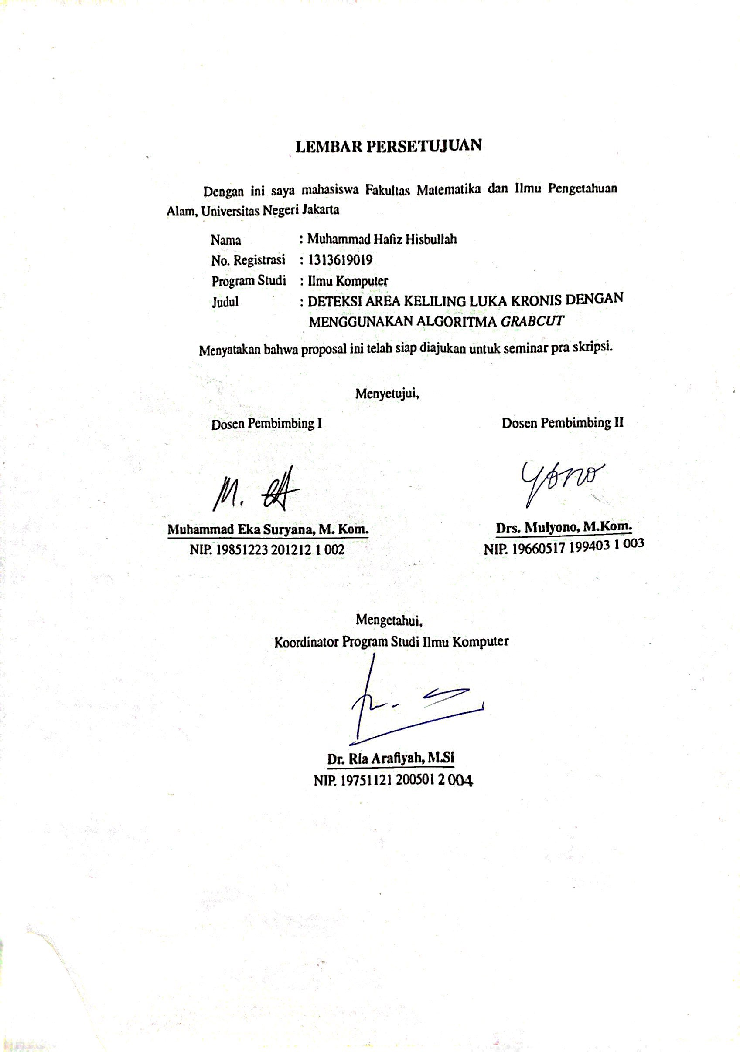
\includepdf[pages=-]{Lembar_Pengesahan.pdf}

\chapter*{\centering{\large{LEMBAR PERSETUJUAN}}}
\thispagestyle{empty} {\bf }Dengan ini saya mahasiswa Fakultas
Matematika dan Ilmu Pengetahuan Alam, Universitas Negeri Jakarta

\vskip3mm

\begin{tabular}{ll}
  Nama & : Muhammad Hafiz Hisbullah \\
  No. Registrasi & : 1313619019 \\
  Program Studi & : Ilmu Komputer \\
  Judul & :  DETEKSI AREA KELILING LUKA KRONIS DENGAN \\ & \hspace{0.2cm} MENGGUNAKAN ALGORITMA \emph{GRABCUT}\\
\end{tabular}

\vskip3mm

% \noindent \hskip10mm Menyatakan bahwa proposal ini telah siap diajukan untuk seminar pra skripsi.
\begin{center}
Menyatakan bahwa skripsi ini telah siap diajukan untuk sidang skripsi.
\end{center}



\begin{center}
\vskip3mm

Menyetujui,

\vskip3mm
\begin{spacing}{1.25}

\begin{tabular}{ccc}
  \hskip-2mm Dosen Pembimbing I & \qquad \qquad \qquad \qquad \qquad & \hskip-6mm Dosen Pembimbing II \\
   &  &  \\
   &  &  \\
   &  &  \\
   &  &  \\
  \hskip-2mm \underline{\textbf{Muhammad Eka Suryana, M. Kom.}} &  & \hskip-6mm \underline{\textbf{Drs. Mulyono, M.Kom.}} \\
  \hskip-2mm NIP. 19851223 201212 1 002 &  & \hskip-6mm NIP. 19660517 199403 1 003	 \\
\end{tabular}
\end{spacing}
\end{center}
\vskip3mm
\begin{center}
Mengetahui, \\
Koordinator Program Studi Ilmu Komputer
\end{center}
\begin{spacing}{1.25}
{ \ }
\\
\\
{ \ }\begin{center}
\underline{\textbf{Dr. Ria Arafiyah, M.Si}} \\
{NIP. 19751121 200501 2 004}
\end{center}
\end{spacing} 
  
\phantomsection
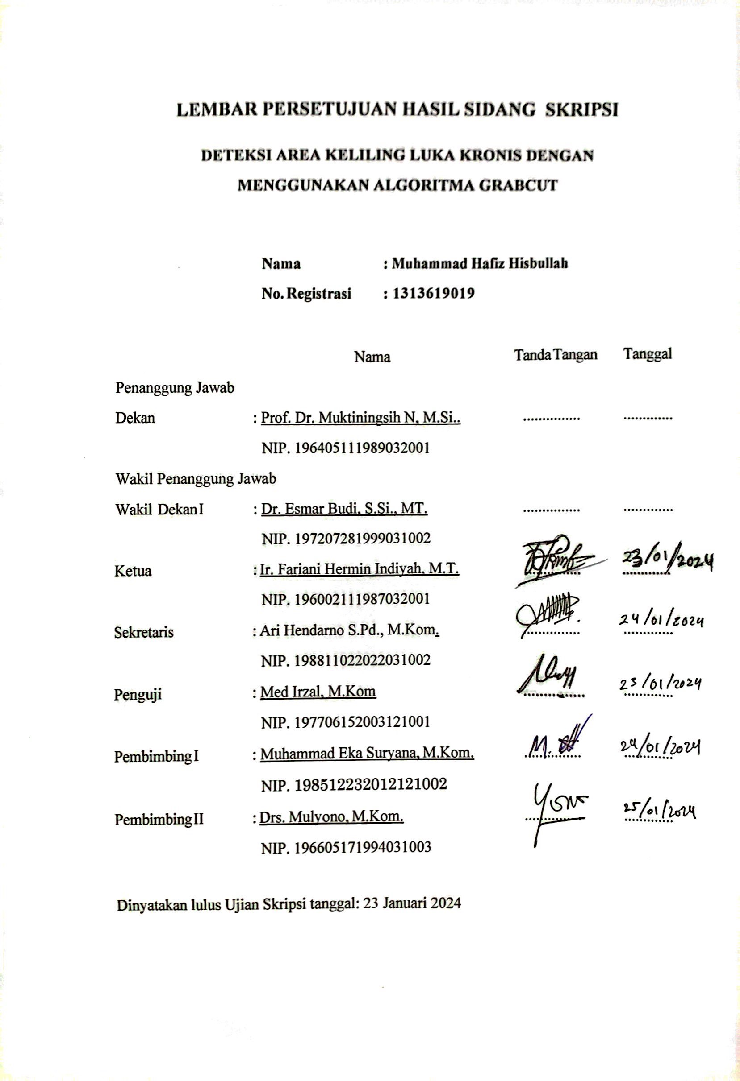
\includepdf[pages=-]{Lembar_Persetujuan_Revisi.pdf}
\addcontentsline{toc}{chapter}{LEMBAR PERSETUJUAN}
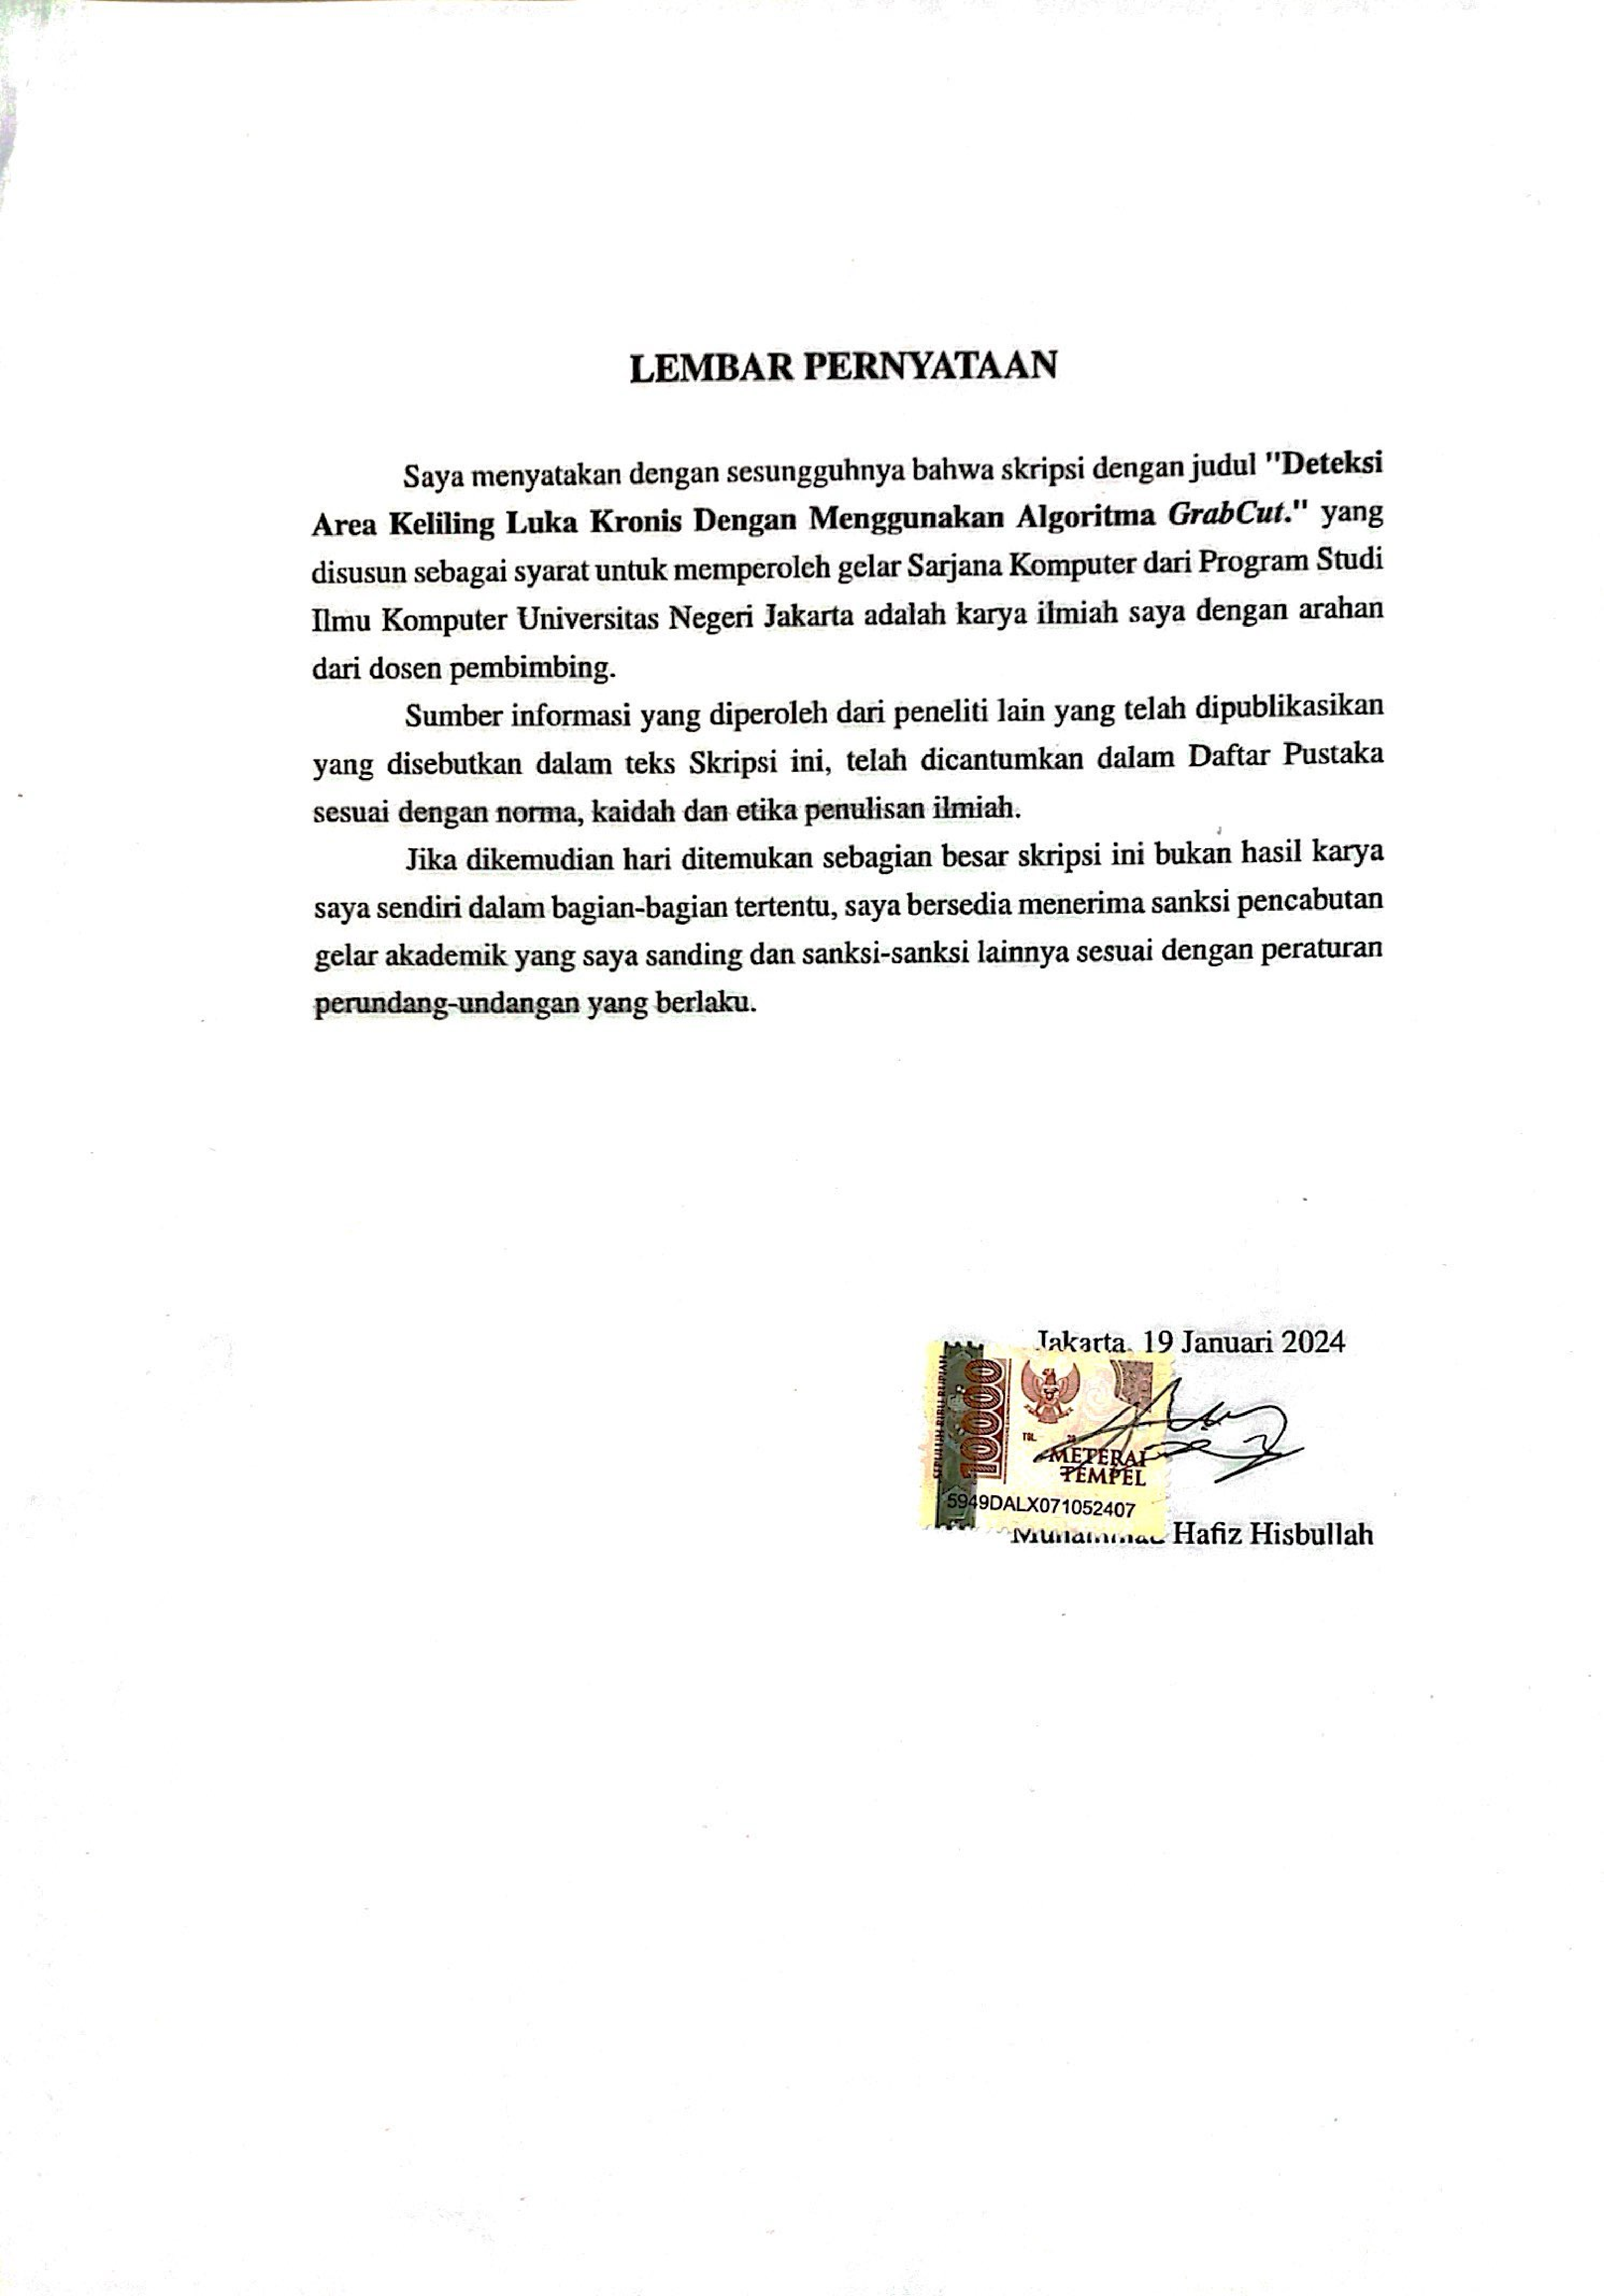
\includepdf[pages=-]{Lembar_Pernyataan.pdf}
\addcontentsline{toc}{chapter}{LEMBAR PERNYATAAN}
\chapter*{\centering{\large{KATA PENGANTAR}}}
\onehalfspacing{}
Dengan penuh syukur, penulis ingin mengungkapkan rasa terima kasih kepada Allah SWT, 
atas berkat-Nya yang memungkinkan penulis menyelesaikan proposal skripsi berjudul 
\textit{DETEKSI AREA KELILING LUKA KRONIS DENGAN MENGGUNAKAN ALGORITMA GRABCUT}.

Semoga penghargaan ini mencerminkan segenap rasa syukur penulis atas bimbingan, 
dorongan, dan inspirasi yang telah diberikan. Harapannya, tugas akhir ini dapat 
memberikan manfaat yang nyata bagi semua pihak yang terlibat, dan khususnya, dapat 
menjadi langkah maju dalam peningkatan pengetahuan dan pemahaman dalam bidang yang 
diteliti. Penulis juga berdoa semoga Allah SWT senantiasa membalas kebaikan dan 
keikhlasan dari semua pihak yang telah turut serta membantu hingga proposal skripsi 
ini mencapai kesempurnaan.

\begin{enumerate}

	\item{Yth. Para petinggi di lingkungan FMIPA Universitas Negeri Jakarta.}
	\item{Yth. Ibu Dr. Ria Arafiyah, M.Si selaku Koordinator Program Studi Ilmu
		Komputer.}
	\item{Yth. Bapak Muhammad Eka Suryana, M.Kom selaku Dosen Pembimbing I yang
		telah membimbing, mengarahkan, serta memberikan saran dan koreksi terhadap
		proposal skripsi ini.}
	\item{Yth. Bapak Drs. Mulyono, M.Kom selaku Dosen Pembimbing II yang telah
		membimbing, mengarahkan, serta memberikan saran dan koreksi terhadap
		proposal skripsi ini.}
	\item{Kedua orang tua dan kakak penulis yang telah mendukung dan memberikan 
		semangat serta doa untuk penulis.}
	\item{Teman-teman Program Studi Ilmu Komputer 2019 yang telah memberikan 
		dukungan dan memiliki andil dalam penulisan proposal skripsi ini.}
	
\end{enumerate}

Dengan penuh kesederhanaan, penulis mengakui bahwa dalam penyusunan proposal skripsi 
ini, belum mencapai kesempurnaan karena terbatasnya pengetahuan dan pengalaman 
yang dimiliki. Karena itulah, penulis dengan hati yang lapang menerima kritik 
serta saran yang konstruktif, yang datang bagai bunga-bunga pengharapan.

Sebagai perjalanan ini mencapai akhir, penulis mengharapkan tugas akhir ini akan 
menjadi ladang berkah bagi semua pihak yang terlibat, tak terkecuali diri penulis 
sendiri. Dalam doa yang dipanjatkan, semoga Allah SWT selalu melipatgandakan kebaikan 
bagi semua yang telah berperan serta membantu penulis meniti jalan menuju puncak 
kesuksesan dalam menyelesaikan proposal skripsi ini.

\vspace{2cm}

\begin{tabular}{p{7.5cm}c}
	&Jakarta, 3 Agustus 2023\\
	&\\
	&\\
	&\\
	&Mochammad Hafiz Hisbullah
\end{tabular}

\addcontentsline{toc}{chapter}{KATA PENGANTAR}
\chapter*{\centering{\large{ABSTRAK}}}
\singlespacing{}

\textbf{MUHAMMAD HAFIZ HISBULLAH}, Deteksi Area Keliling Luka Kronis Dengan 
Menggunakan Algoritma \emph{GrabCut}. Skripsi, Program Studi Ilmu Komputer, Fakultas Matematika dan Ilmu Pengetahuan Alam, Universitas Negeri Jakarta. Januari 2024.
\\
\\
Luka kronis merupakan masalah kesehatan yang kompleks, khususnya bagi pasien dengan 
penyakit seperti Diabetes Melitus (DM). Proses penyembuhan luka melibatkan asesmen 
yang cermat dan pengelolaan yang efektif, namun metode manual dalam pengukuran 
luka seringkali tidak akurat dan memakan waktu. Skripsi ini bertujuan untuk penggunaan 
metode \emph{GrabCut} dalam pemrosesan citra untuk mendeteksi area keliling 
luka kronis. Metode ini memiliki potensi untuk memberikan analisis yang objektif 
dan reliabel dalam asesmen luka. Dengan memanfaatkan teknologi pemrosesan gambar 
dan pembelajaran mesin, kami mencoba mengatasi keterbatasan metode manual dengan 
menggunakan algoritma \emph{GrabCut}. Langkah pertama melibatkan pengambilan foto 
luka menggunakan perangkat seluler, diikuti oleh kalibrasi warna untuk memastikan 
konsistensi. Metode \emph{GrabCut} kemudian diterapkan untuk mengsegmentasi area 
luka, dengan fokus pada pemisahan antara objek utama (luka) dan latar belakang. 
Hasil akhir menunjukkan bahwa data yang berhasil disegmentasi menggunakan \emph{Grabcut}
untuk semua kategori luka sebanyak 70 (dari 71 data) serta menghasilkan rata-rata 
nilai akurasi \emph{Grabcut} 89.36\%, untuk kategori warna luka hitam berhasil 
segmentasi sebanyak 24 (dari 24 data) dengan rata-rata nilai akurasi 91.55\%,
untuk kategori warna luka kuning berhasil segmentasi sebanyak 14 (dari 15 data) 
dengan rata-rata nilai akurasi 82.73\%, kemudian untuk kategori warna luka merah 
berhasil segmentasi sebanyak 32 (dari 32 data) dengan rata-rata nilai akurasi 93.79\%,
\\
\\
\textbf{Kata kunci:} luka kronis, \emph{GrabCut}, pemrosesan citra, asesmen luka, pengelolaan luka.
\addcontentsline{toc}{chapter}{ABSTRAK}
\chapter*{\centering{\emph{\large{ABSTRACT}}}}
\singlespacing{}

\textbf{MUHAMMAD HAFIZ HISBULLAH}, Detection of Chronic Wound Perimeter Using the 
GrabCut Algorithm. Undergraduate Thesis, Computer Science Program, Faculty of 
Mathematics and Natural Sciences, State University of Jakarta. January 2024.
\\

Chronic wounds pose a complex health issue, especially for patients with conditions 
such as Diabetes Mellitus (DM). The wound healing process involves meticulous 
assessment and effective management, yet manual methods in wound measurement often 
prove inaccurate and time-consuming. In this research, we propose the use of the 
GrabCut method in image processing to detect the perimeter of chronic wounds. 
This method has the potential to provide objective and reliable wound assessment.
By leveraging image processing technology and machine learning, we aim to overcome 
the limitations of manual methods by employing the GrabCut algorithm. The first 
step involves capturing wound images using mobile devices, followed by color 
calibration to ensure consistency. The GrabCut method is then applied to classify 
the wound area, focusing on the separation of the main object (the wound) from 
the background. This research utilizes a dataset of chronic wound images from 
previous studies and seeks to compare the results of the GrabCut method with 
reference images as ground truth. It is hoped that this research will contribute 
to the effectiveness of chronic wound assessment, expedite the management process, 
and help alleviate the financial burden on patients.
\\
\\
\textbf{Keywords}: chronic wounds, GrabCut, image processing, wound assessment, wound management.

\addcontentsline{toc}{chapter}{\emph{ABSTRACT}}
\singlespacing{}
\tableofcontents{}
\addcontentsline{toc}{chapter}{DAFTAR ISI}
\listoffigures{}
\addcontentsline{toc}{chapter}{DAFTAR GAMBAR}
\listoftables{}
\addcontentsline{toc}{chapter}{DAFTAR TABEL}

\begin{counterpage}
\end{counterpage}
%Disini awal masukan untuk Bab
%-----------------------------------------------------------------
\onehalfspacing{}
%!TEX root = ./template-skripsi.tex
%-------------------------------------------------------------------------------
% 								BAB I
% 							LATAR BELAKANG
%-------------------------------------------------------------------------------

\chapter{PENDAHULUAN}

\section{Latar Belakang Masalah}

% Intro
Luka merupakan kerusakan atau gangguan  yang terjadi pada stuktur anatomi kulit. 
Hal ini sering kita temui pada permukaan kulit atau pada integritas epitel kulit,
luka berkisar dari kerusakan yang bervariasi mulai dari kerusakan sederhana atau
terjadi lebih dalam, bahkan bisa saja meluas ke jaringan subkutan yang berdampak 
pada struktur lain seperti tendon, pembuluh darah, otot, saraf, organ parenkim, dan 
hingga sampai tulang. Luka timbul karena adanya proses patologis secara internal 
maupun eksternal, apapun penyebab dan bentuknya, luka dapat merusak jaringan dan 
mengganggu sistem yang ada didalamnya, respon yang ditimbulkan oleh luka secara 
fisiologis di antaranya menyebabkan pendarahan, kontraksi pembuluh darah dengan 
koagulasi, aktivasi komplemen serta respon inflamasi (\cite{Velnar:2009}).


% Klasifikasi luka
Luka dapat diklasifikasikan dalam berbagai kriteria. Berdasarkan waktu penyembuhan 
luka dibagi menjadi dua, yaitu luka akut dan luka kronis. ~\cite{Velnar:2009} dalam 
penelitiannya mengatakan luka akut adalah luka yang dapat penyembuhan secara mandiri 
dan berlangsung secara normal dengan proses penyembuhan yang membutuhkan waktu yang 
teratur, luka akut berakhir dengan hasil dari restorasi fungsi anatomis. 
Luka kronis ialah luka yang proses penyembuhannya gagal berjalan dengan normal, 
proses penyembuhan luka kronis tidak dapat diperbaiki dengan cepat dan teratur, 
hal ini dikarenakan adanya gangguan oleh beberapa faktor dalam tahap fase hemositasis, 
peradangan, proliferasi atau \emph{remodelling}. Luka kronis dapat disebabkan oleh berbagai 
penyebab, di antaranya naturopati, tekanan, insufisiensi arteri dan vena, diabetes melitus, 
luka bakar dan vaskulitis.


% Penyembuhan luka
Proses penyembuhan luka adalah proses kompleks dengan serangkaian interaksi beragan 
antara sistem imunologi dan biologis, penyembuhan luka ini terdiri dari berbagai 
fase dengan langkah dan peristiwa yang berlangsung dengan perlahan dan dilakukan 
secara sistematis sehingga muncul berbagai jenis sel badi dasar luka selama proses 
penyembuhan berlangsung (\cite{Velnar:2009}). Ketika seseorang mengalami luka 
dibagian jaringan kulit, penanganan yang biasanya dilakukan adalah menutup luka 
tersebut agar tidak terjadi pendarahan terus menerus, hal tersebut bisa dilakukan 
jika luka yang dialami ialah luka kecil dan hanya dipermukaan saja, namun jika luka 
tersebut merupakan luka kronis, maka disarankan untuk melakukan penanganan dan pengkajian 
ke rumah sakit agar segera dilakukan tindakan oleh dokter atau perawat.  


% luka kronis
Luka kronis menjadi salah satu permasalahan bagi beberapa pihak. Bagi pasien yang 
memiliki luka kronis khususnya akibat penyakit Diabetes Melitus (DM) akan menghabiskan 
banyak biaya dalam pengobatannya. \cite{Wang:2015} dalam penelitiannya menyebutkan 
di Amerika Serikat jutaan pasien penderita luka kronis mengeluarkan miliaran uang 
tiap tahunnya,  pasien penderita luka kronis akibat Diabetes Melitus (DM) saja bisa 
menghabiskan 38 miliar dolar, kebanyakan di antaranya biaya rawat inap dan operasi di 
rumah sakit, dan biaya perawatan jangka panjang yaitu perawatan dari rumah secara 
berkala. Di Amerika tercatat jumlah pasien penderita diabetes mencapai 20 juta dan 
diperkirakan pada tahun 2030 jumlahnya akan naik dua kali lipat (\cite{Han:2017}). 
Tentu saja dengan jumlah begitu banyak maka perawat dan rumah sakit yang menangani 
perawatan luka akan memakan banyak waktu  dan mengeluarkan banyak biaya (\cite{Wang:2015}), 
hal ini mengakibatkan tenaga perawat yang menangani pasien penderita luka kronis 
membutuhkan banyak waktu. 


% Tahapan penyembuhan
Proses penyembuhan luka terjadi dalam beberapa tahapan, seorang perawat luka wajib 
memberikan asesmen perawatan luka sesuai prosedur medis agar keadaan luka segera 
membaik dan menghindari terjadnya infeksi. Proses penyembuhan yang dilakukan pertama 
kali ialah membersihkan dan dibalut dengan benar, setelah luka dibersihkan maka 
akan dilakukan metode debridemen luka, hal ini bertujuan untuk mengangkat jaringan 
(nektrotik) yang mati, terinfeksi dan penebalan pada jaringan kulit (hiperkeratoris), 
membentuk dasar penyembuhan luka. Debridemen memiliki fungsi yang penting dalam 
asesmen luka karena akan mempercepat proses penyembuhan luka, debridemen yang ada 
pada luka kronis berfungsi sebagai penanganan kelainan medis dan mengubah kronis 
tersebut menjadi luka akut, setelah menjadi luka akut maka penyembuhan akan kembali 
normal (\cite{Velnar:2009}).


% Asesmen luka
Proses asesmen luka dilakukan bertahap, tindakan yang diberikan tiap tahap penyembuhan 
dilakukan berdasarkan kajian evaluasi luka, kajian ini memantau proses penyembuhan 
luka secara berkala (\cite{Silva:2021}). Metode evaluasi luka biasanya menggunakan 
metode invasif (kontak) dan non-invasif (non-kontak) (\cite{ManoharDhane:2017}).

Hal penting yang dijadikan sebagai indikator untuk penyembuhan luka ialah dengan 
memperhatikan ukuran luka, di antaranya perubahan luas, kedalaman dan jenis jaringan 
yang luka (\cite{Silva:2021}). Seorang perawat luka melakukan inspeksi kontak 
luka dengan mengukur luka dilakukan secara manual yaitu dengan bantuan penggaris 
luka dan label perekat yang bersentuhan langsung dengan luka, dalam penelitiannya 
\cite{Silva:2021} menyebutkan teknik ini cenderung dapat menyebabkan resiko infeksi, 
mengganggu kenyamanan dan memperburuk kondisi klinis pasien, ditambah penggunaan 
teknik-teknik tersebut tidak akurat, tidak konsisten, dan tentu mengalami kekurangan 
standar penilaian. Standar pengukuran dengan metode manual tersebut memiliki tingkat 
kesalahan yang cukup tinggi yaitu sekitar 44 persen  (\cite{Rizki:2022}).


Para ilmuwan telah banyak melakukan penelitian mengenai hal ini, agar proses asesmen 
dan kajian luka dapat dilakukan secara efektif dan efisien mulai dari waktu, tenaga, 
hingga pengeluaran biaya yang cukup banyak, teknologi dibidang pemrosesan citra gambar 
menjadi hal yang memungkinkan saat ini untuk dikembangkan, dengan menggunakan pemrosesan 
gambar yang dibantu oleh pembelajaran mesin memungkinkan melakukan analisis gambar 
luka oleh program komputer (\cite{Wang:2015}). 


\cite{Silva:2021} berpendapat bahwa pengembangan citra digital untuk melakukan 
evaluasi luka merupakan alternatif yang sangat penting, teknik ini akan menginformasikan 
analisis yang lebih objektif dan reliabel. Mereka melakukan penelitian mengenai 
pengusulan untuk menentukan area luka dengan menggunakan pengklasifikasi berbasis 
citra medis yaitu  \emph{Support Vector Mechine} (SVM) serta mengkombinasikannya dengan 
metode \emph{GrabCut} untuk segmentasi area yang terkena luka. Metode segmentasi gambar 
ini sepenuhnya otomatis serta perawat tidak perlu melakukan kontak langsung dengan 
objek, tingkat akurasinya diperkirakan mencapai 96 persen, sensitifitas sebesar 94 persen, 
spesifisitas 97 persen, tingkat presisi 94 persen dan interaksi penyatuan 89 persen.


Langkah pertama seorang perawat dalam melakukan asesmen luka digital ialah dengan 
mengambil foto luka menggunakan kamera telepon pintar atau tablet nya, ketika ada 
dua foto dengan pose yang sama namun dengan perangkat kamera yang berbeda, warna 
yang dihasilkan kemungkinan akan berbeda. Untuk menangani hal tersebut adalah setiap 
kamera menggunakan \emph{device independent} sRGB. Zaman sekarang sudah banyak vendor kamera 
telepon pintar menyediakan mode ini namun dengan pengaturan pewarnaan RGB mereka 
masing-masing. Oleh karena ini dibutuhkan adanya kalibrasi dengan melakukan 
transformasi citra menjadi ruang warna CIE, kemudian menjadi sRGB dengan serangkaian 
optimalisasi (\cite{Rizki:2022}).

\cite{Silva:2021} menjelaskan dalam karyanya bahwa parameter yang digunakan untuk 
segmentasi daerah yang terkena luka ialah perbedaan warna antara kulit dan luka, 
berdasarkan ambang batas semi otomatis dalam ruang pewarnaan RGB, 
\cite{ManoharDhane:2017} menggunakan metode pengelompokan spektral fuzzy untuk segmentasi warna 
berdasarkan tingkat kesamaan fuzzy (tingkat abu-abu) yang dihitung di atas gambar, 
hasil menunjukkan pada 70 gambar mencapai akurasi 92 persen, sensitifitas 87 persen, dan spesifisitas 96 persen.


Sebenarnya ada beberapa metode yang bisa digunakan untuk melakukan image processing 
dengan bantuan \emph{Support Vector Mechine} (SVM) seperti kesamaan fuzzy, \emph{active contour} 
(snake), dan \emph{region-of-interest} (ROI), dan \emph{GrabCut}. Metode-metode yang pernah dilakukan 
merupakan pendekatan untuk menghasilkan objek luka yang akurat \cite{Garcia-Zapirain:2017}. 
Beberapa di antara metode yang disebutkan juga memiliki keterbatasan yang beragam, 
mulai dari inisiasi awal gambar yang manual, atau intensitas warna yang bergantung 
dari intensitas gradien. 


\cite{Rizki:2022} dalam penelitiannya yaitu pendeteksi luka menggunakan metode 
\emph{active contour} (snake) dan \emph{active contour} (snake) dengan ditambah 
interpolasi, dalam penelitiannya mencari  \emph{ground truth} dalam objek-objek gambar 
luka pasien, ketika dilakukan pemrosesan gambar dengan metode yang dijalankan, \emph{ground truth} menunjukkan hasil yang kurang maksimal dimana hasil dari deteksi 
luka dengan metode snake versi integer hanya berhasil menutupi luka berjumlah 
12 data dari total 71 data yang tersedia, sedangkan metode snake interpolasi 
berjumlah 44 data dari total 71 data yang tersedia. \cite{Silva:2021} melakukan 
penelitian mengenai pengolahan citra gambar dengan menggunakan \emph{Support Vector Mechine} 
(SVM) dengan menggunakan \emph{GrabCut}, dalam tulisannya menerangkan bagaimana cara segmentasi 
gambar luka dengan menggunakan \emph{GrabCut},  setidaknya ada lima tahapan dalam prosesnya, 
di antaranya segmentasi superpiksel, ekstraksi fitur, persiapan data, klasifikasi 
dan terakhir yaitu segmentasi luka. 


Segmentasi superpiksel merupakan teknik untuk merepresentasi ringkas dari gambar 
menjadi kelompok piksel yang lebih kecil sesuai dengan spasial dan kriteria warna. 
Segmentasi superpiksel  ini digunakan oleh beberapa metode di antaranya SEED, LSC 
dan SLIC. Metode ini menghasilkan beberapa informasi dari gambar luka seperti tepi 
luka dan parameter yang digunakan untuk metode selanjutnya (\cite{Silva:2021}). 
\cite{Wang:2015} menggunakan gambar berukuran 480 x 640 piksel, hal ini dikarenakan 
untuk memangkas biaya komputasi dalam pemrosesan, sampel diambil secara acak, sementara 
SVM linier untuk melatih data yang tersedia. Setelah data telah tersegmentasi menjadi 
superpiksel, maka dilakukan proses klasifikasi dengan menggunakan \emph{Support Vector 
Mechine} (SVM), hal ini diperlukan karena pada ditahap ini banyak terdapat superpiksel 
berada di sekitar luka pada kulit dan dikhawatirkan dapat salah dalam klasifikasi 
sehingga menurunkan tingkat akurasi segmentasi. Proses selanjutnya dalam pengolahan 
citra gambar luka ialah segmentasi luka, salah satu metode yang paling populer untuk 
segmentasi citra gambar ialah menggunakan algoritma \emph{GrabCut}, teknik ini merupakan 
teknik yang bekerja berdasarkan analisis statistik serta teori grafik, hal ini 
bertujuan untuk memisahkan suatu objek inti gambar dari objek sisa di sekitar gambar, 
pada akhirnya data telah menghasilkan suatu objek citra yang berisi area luka beserta 
komponen yang ada pada data tersebut. (\cite{Nugraha:2022}) menggunakan metode 
\emph{GrabCut} dalam penelitiannya mengenai ekstraksi latar depan citra ikan, hasil yang 
didapatkan dari dataset untuk dilakukan uji coba bahwa apabila \emph{GrabCut} diuji pada 
data citra multi objek, maka objek yang ada pada data tersebut akan gagal diseleksi 
oleh \emph{GrabCut}, namun jika data tersebut hanya terdapat satu objek maka \emph{GrabCut} berhasil 
melakukan seleksi citra dengan baik dan menghasilkan data yang bagus.


Di dalam penelitian ini, penulis akan melakukan penerapan algoritma \emph{GrabCut} pada 
pemrosesan citra gambar yang akan menghasilkan segmentasi area luka, metode yang 
penulis pilih berdasarkan hasil dari penelitian Muhammad Rizki dimana \emph{ground truth} (area sebenarnya) 
yang dihasilkan lebih banyak yang gagal dibandingkan yang berhasil, sehingga penulis 
tertarik untuk mengganti metode yang dijalankan untuk segmentasi area keliling luka 
kronis. Selain itu penulis memilih metode \emph{GrabCut} untuk dijadikan sebagai 
penelitian dikarenakan metode ini sangat cocok untuk citra gambar luka dimana yang 
merupakan citra satu objek \emph{(single object)}. Tahap pertama penulis akan menandai 
daerah yang mencakup objek luka, kemudian objek akan dilakukan pengujian metode 
\emph{GrabCut} pada citra tunggal (\emph{single object}). Dalam penelitian ini 
penulis akan menggunakan dataset citra yang tersedia di repositori \emph{https://github.com/mekas/InjuryDetection.}
Dataset citra ini berasal dari penelitian luka Ns. Ratna Aryani M.Kep, tahun 2018 
(\cite{Aryani:2018}). Diharapkan dalam penelitian ini mendapatkan hasil berupa nilai 
akurasi antara metode \emph{GrabCut} dengan hasil citra referensi.

\section{Rumusan Masalah}
Berdasarkan uraian pada latar belakang yang diutarakan di atas, maka perumusan 
masalah pada penelitian ini adalah Bagaimana cara mendeteksi keliling luka dengan 
menggunakan metode \emph{GrabCut}?

\section{Pembatasan Masalah}
Adapun beberapa pembatasan telah diterapkan dalam penelitian ini guna menjaga fokus 
pada permasalahan yang dijelaskan sebelumnya. Berikut adalah batasan-batasan yang 
telah diterapkan:

\begin{enumerate}
	\item Mendeteksi area keliling luka kronis menggunakan metode \emph{GrabCut} dengan data 
	citra luka yang didapat dari penelitian luka Ns. Ratna Aryani, M.Kep, tahun 2018. 
	\item Penelitian ini hanya berfokus pada pemisahan antara objek utama dan 
	latar belakang pada citra gambar luka.
	\item Objek utama, yaitu area luka, diharapkan hanya terdapat satu area luka pada setiap citra.
	\item Citra-citra yang digunakan dalam penelitian ini adalah citra digital yang menggunakan sistem warna RGB.
	\item Ukuran panjang citra yang dijadikan objek penelitian adalah 320 piksel.
	\item Bahasa pemrograman yang digunakan dalam penelitian ini adalah Python v 3.9
\end{enumerate}

\section{Tujuan Penelitian}
Penelitian ini bertujuan untuk membuat sistem untuk mendeteksi objek luka pada citra luka
dengan menggunakan metode \emph{GrabCut}.

\section{Manfaat Penelitian}
\begin{enumerate}
	\item Bagi Penulis
	\begin{itemize}
		\item Meningkatkan wawasan dan pengalaman praktis terkait deteksi latar 
		depan pada citra luka melalui penggunaan metode \emph{GrabCut}.

		\item Untuk memenuhi persyaratan kelulusan dalam program Sarjana (S1) di 
		Program Studi Ilmu Komputer, Fakultas Matematika dan Ilmu Pengetahuan Alam, 
		Universitas Negeri Jakarta
	\end{itemize}
		
	\item Bagi Instansi Terkait
	
	Metode yang diajukan diharapkan dapat membuka peluang untuk diajukan ke instansi 
	kesehatan terkait dalam proses pengkajian luka kronis.

	\item Bagi Ilmu Pengetahuan

	\begin{itemize}
		\item Mahasiswa
		
		Penulis berharap penelitian ini dapat digunakan sebagai sumber penunjang 
		referensi, khususnya Pustaka tentang deteksi keliling luka kronis dengan 
		menggunakan metode \emph{GrabCut}.

		\item Bagi Peneliti Selanjutnya
	
		Diharapkan penelitian ini dapat digunakan sebagai dasar atau kajian awal 
		bagi peneliti lain yang ingin meneliti permasalahan yang sama.
	\end{itemize}

	\item Bagi Universitas Negeri Jakarta
	
	Menjadi pertimbangan dan evaluasi akademik khususnya Program Studi Ilmu Komputer 
	dalam penyusunan skripsi sehingga dapat meningkatkan kualitas akademik di program 
	studi Ilmu Komputer Universitas Negeri Jakarta serta meningkatkan kualitas lulusannya.
			
\end{enumerate}

% Baris ini digunakan untuk membantu dalam melakukan sitasi
% Karena diapit dengan comment, maka baris ini akan diabaikan
% oleh compiler LaTeX.
\begin{comment}
\bibliography{daftar-pustaka}
\end{comment}
 %!TEX root = ./template-skripsi.tex
%-------------------------------------------------------------------------------
%                            BAB II
%               KAJIAN TEORI
%-------------------------------------------------------------------------------

\chapter{KAJIAN PUSTAKA} 

\section{Citra Gambar Digital}

Sebuah gambar dapat diberikan definisi sebagai fungsi dua dimensi \(f(x, y)\), 
dimana x dan y mewakili koordinat ruang (bidang) dan amplitudo f pada setiap 
pasangan koordinat \((x, y)\) merujuk pada intensitas atau level keabuan citra pada 
koordinat tersebut. Jika x, y, dan nilai intensitas f semuanya terbatas \emph{(finite)} 
dan memiliki nilai diskret, maka gambar tersebut dianggap sebagai gambar digital. 

Dalam hal ini, fungsi \emph{f(s, t)} merujuk pada fungsi gambar kontinu dengan dua variabel 
kontinu s dan t. Fungsi ini kemudian diubah menjadi gambar digital melalui proses \emph{sampling} 
dan kuantisasi. Melalui proses ini, sampel-sampel dari gambar kontinu diubah menjadi 
gambar digital \(f(x, y)\). Gambar digital dapat direpresentasikan dalam 
bentuk matriks \emph{(array)} yang terdiri dari nilai-nilai numerik \(f(x, y)\).

\begin{equation} \label{eq:array_citra}
  f(x,y) = 
  \begin{bmatrix}
    f(0,0) & f(0,1) & \cdots & f(0, N-1)\\
    f(1,0) & f(1,1) & \cdots & f(1, N-1)\\
    \vdots & \vdots & \vdots & \vdots\\
    f(M-1,0) & f(M-1,1) & \cdots & f(M-1,N-1)
  \end{bmatrix}
\end{equation}

Matriks \emph{(array)} diatas adalah representasi yang digunakan dalam pengolahan 
komputer (\cite{Gonzalez:2018}), dimana

\begin{conditions}
  f(x,y) & Fungsi gambar citra digital\\
  M & Banyaknya baris\\
  N & Banyaknya kolom\\
  x & 0, 1, 2, . . . , M - 1\\
  y & 0, 1, 2, . . . , N - 1
\end{conditions}

Sebuah citra digital merupakan sejumlah elemen yang memiliki batasan \emph{(finite)}, 
dan setiap elemen ini memiliki nilai dan posisi tertentu. Setiap elemen dari array 
ini disebut sebagai elemen gambar, elemen citra, piksel, atau pel. Piksel-piksel 
tertentu merepresentasikan nilai-nilai dalam array yang terletak pada pasangan 
koordinat (\(x,y\)) yang tetap. Piksel merupakan istilah yang paling umum digunakan 
untuk merujuk pada elemen-elemen citra digital (\cite{Gonzalez:2018}).

\section{Pemrosesan Citra Digital}
Pemrosesan gambar digital adalah proses yang dilakukan pada citra sebagai masukan
dengan melalui beberapa tahapan seperti pra-pemrosesan citra tersebut, mengekstrak 
(memsegmentasi) elemen, mendeskripsikan elemen dalam bentuk yang sesuai 
untuk pemrosesan citra tersebut.

\cite{Gonzalez:2018} menyebutkan bahwa pemrosesan citra digital dapat dikelompokkan 
menjadi tiga tingkatan, yakni rendah, menengah, dan tinggi. Pada tingkat pengolahan 
rendah, dilakukan operasi dasar seperti pra-pemrosesan citra guna mengurangi \emph{noise}, 
mempertajam kontras, serta memperjelas citra. Proses ini memfokuskan pada citra 
sebagai input maupun outputnya. Pengolahan tingkat menengah pada citra melibatkan 
langkah-langkah seperti membagi citra menjadi wilayah atau objek (segmentasi), 
menguraikan objek dalam citra untuk disesuaikan dengan pemrosesan komputer, dan 
mengenali objek secara keseluruhan. Pengolahan tingkat menengah ditandai oleh 
masukan yang umumnya berupa citra, dengan hasil keluaran berupa atribut yang 
diekstraksi dari citra tersebut (contohnya, tepi, kontur, dan identitas objek).
Akhirnya, pada tingkat pengolahan citra yang lebih tinggi, terdapat pengenalan 
objek dalam citra.

\section{Citra Gambar Berwarna}

\cite{Gonzalez:2018} dalam bukunya mengatakan bahwa Warna yang kita lihat pada objek 
dipengaruhi oleh cahaya yang dipantulkannya. Cahaya terlihat terdiri dari spektrum 
sempit dalam spektrum elektromagnetik. Objek yang memantulkan cahaya merata pada 
semua panjang gelombang terlihat putih, sementara yang memantulkan dalam rentang 
tertentu terlihat berwarna. Contohnya, objek hijau memantulkan cahaya dengan panjang 
gelombang 500-570 nm, menyerap pada panjang gelombang lainnya.

\begin{figure}[H]
	\centering{}
	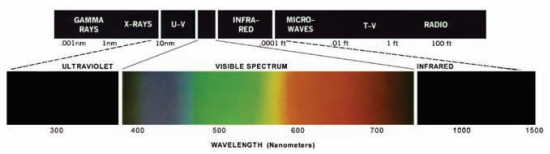
\includegraphics[width=\textwidth]{gambar/gelombang_cahaya.png}
	\caption{Spektrum cahaya, (\cite{Gonzalez:2018})}
\end{figure}

Mata manusia memiliki sel kerucut yang sensitif terhadap warna. Sekitar 65\% sensitif 
terhadap merah, 33\% terhadap hijau, dan hanya 2\% terhadap biru. Meskipun jarang, 
sel biru sangat sensitif. Sel-sel ini menyerap cahaya dengan karakteristik berbeda, 
sehingga mata kita melihat warna dengan gabungan merah (R), hijau (G), dan biru (B).

\begin{figure}[H]
	\centering{}
	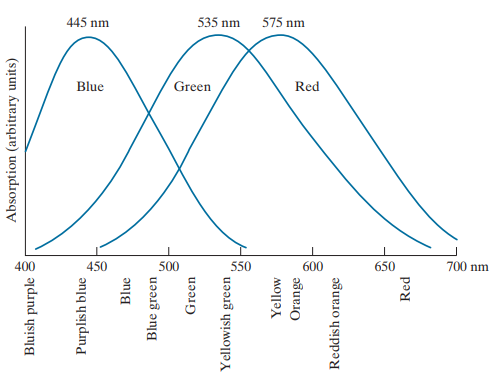
\includegraphics[width=0.8\textwidth]{gambar/gelombang_rgb_mata.png}
	\caption{Penyerapan cahaya yang ditangkap oleh mata dalam bentuk panjang gelombang, (\cite{Gonzalez:2018})}
\end{figure}

CIE menetapkan standar warna pada 1931, tetapi data eksperimental yang lebih akurat 
muncul pada 1965. Standar CIE hanya sekitar cocok dengan data eksperimental. 
Standar ini menetapkan panjang gelombang biru = 435,8 nm, hijau = 546,1 nm, dan 
merah = 700 nm sebagai warna primer.

Citra gambar yang direpresentasikan kedalam model warna RGB terdiri dari tiga bagian 
yang mewakili warna dasar: merah, hijau, dan biru. Ketika gambar ini ditampilkan di 
layar, ketiga bagian ini bergabung untuk membentuk gambar berwarna. Kita menyebutnya 
model warna RGB karena ini adalah singkatan dari \emph{Red} (merah), \emph{Green} 
(hijau), dan \emph{Blue} (biru). Setiap bagian gambar ini memerlukan sejumlah "bit" 
(ini seperti blok kecil yang menyimpan informasi), dan jumlah bit yang digunakan 
untuk setiap bagian piksel ini disebut "kedalaman piksel". Jika kita memiliki gambar 
RGB dengan setiap bagian (merah, hijau, dan biru) menggunakan 8 bit, maka setiap 
"piksel warna" dalam gambar ini (yang memiliki tiga nilai, satu untuk merah, satu 
untuk hijau, dan satu untuk biru) akan menggunakan total 24 bit (8 bit untuk merah + 
8 bit untuk hijau + 8 bit untuk biru).

\begin{figure}[H]
	\centering{}
	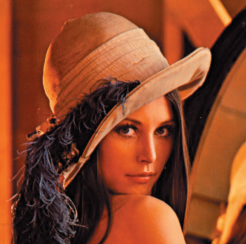
\includegraphics[width=0.4\textwidth]{gambar/gambar_citra_warna.png}
	\caption{Gambar citra berwarna, (\cite{Gonzalez:2018})}
\end{figure}

Gambar berwarna penuh sering disebut gambar RGB 24-bit. Ini artinya setiap piksel 
dalam gambar memiliki 24 bit untuk menyimpan informasi warnanya. Jumlah total warna 
yang bisa direpresentasikan dalam gambar RGB 24-bit sangat besar, sekitar 16 juta 
warna yang berbeda (\cite{Gonzalez:2018}).

\begin{figure}[H]
	\centering{}
	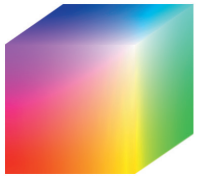
\includegraphics[width=0.4\textwidth]{gambar/rgb_cube.png}
	\caption{24 bit kubus warna RGB, (\cite{Gonzalez:2018})}
\end{figure}

Untuk citra gambar digital, rentang nilai dalam kubus diukur dalam angka yang dapat 
direpresentasikan oleh jumlah bit dalam gambar. Jika, seperti di atas, gambar utama 
adalah gambar 8-bit, batas kubus sepanjang setiap sumbu menjadi [0, 255]. 
Sebagai contoh, warna putih akan berada pada titik [255, 255, 255] dalam kubus.

\section{Pemodelan Distribusi \emph{Gaussian Mixture Model}}

GMM (\emph{Gaussian Mixture Model}) adalah sebuah metode statistik yang dapat digunakan 
untuk memodelkan data sebagai kombinasi beberapa distribusi Gauss. Metode ini 
digunakan dalam segmentasi gambar untuk memodelkan gambar dalam bentuk gabungan 
dari distribusi Gaussian. GMM digunakan untuk memperkirakan probabilitas piksel 
yang termasuk ke dalam objek yang ingin di-segmentasi dan probabilitas piksel 
yang termasuk ke dalam latar belakang. 

\cite{Power:2002} dalam penelitiannya mengatakan setiap piksel terhadap objek diberi \emph{state} dari himpunan \(K\), di mana \(K\) 
adalah jumlah konstan biasanya antara 3 dan 7, \cite{Rother:2004} memberikan nilai \(K = 5\) . Beberapa \emph{state} \(K\) mewakili 
objek latar belakang sedangkan sisanya dianggap sebagai objek depan. \(\omega_k = P(k), k = 1,2,...,K,\) yang menunjukkan 
probabilitas priori munculnya permukaan \(k\) dalam pandangan piksel yaitu:

\begin{equation} \label{eq:prior_probability}
  \Sigma_{k=1}^{K} \: \omega_k = 1
\end{equation}
dimana, 

\begin{conditions}
  K & Parameter konstanta\\
  \omega_k & Probabilitas priori
\end{conditions}

Proses yang menghasilkan \emph{state} permukaan \(k\) tidak dapat di amati langsung dan hanya 
dapat di amati secara tidak langsung melalui nilai piksel terkait X. Bahkan jika 
kita tahu permukaan k yang sedang dilihat, nilai piksel masih memiliki distribusi 
\(f(X|k)\) karena faktor-faktor seperti perubahan pencahayaan, noise kamera, atau 
tekstur permukaan. Nilai piksel merupakan sampel dari variabel acak X yang mencakup 
perilaku k. X dapat berupa satu dimensi (intensitas monokrom), dua dimensi (ruang 
warna), tiga dimensi (warna), atau n-dimensi secara umum. 

peneliti membuat ilustrasi dari parameter gaussian dalam bentuk kurva yang berdistribusi 
normal dalam satu dimensi:

\begin{figure}[H]
	\centering{}
	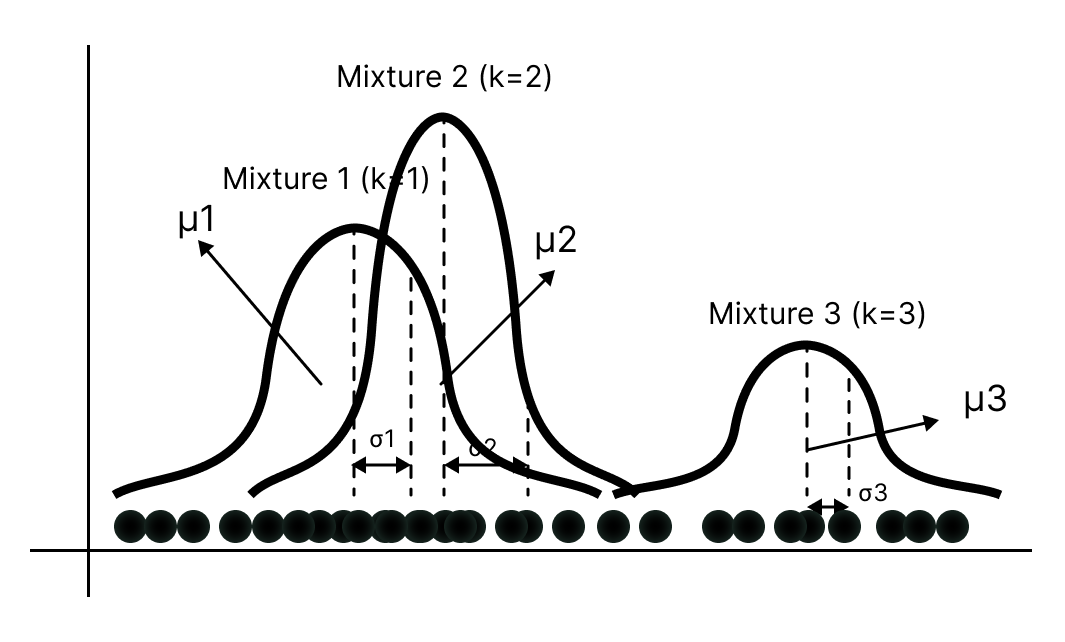
\includegraphics[width=0.8\textwidth]{gambar/gmm_curve.png}
	\caption{Contoh distribusi tiga fungsi gaussian 1 dimensi dengan parameter K = 3, (\cite{Power:2002})}
\end{figure}

Terlihat bahwa terdapat tiga fungsi gaussian, dengan parameter K = 3. Setiap gaussian
menjelaskan data-data yang terdapat pada tiga \emph{mixture} yang ada. 

Untuk memecahkan masalah segmentasi latar depan, \emph{state} k yang paling mungkin 
diestimasi pada setiap waktu sampel \(t\) dari sekelompok observasi yang diambil dari X, 
beserta prosedur untuk membedakan antara \emph{state} latar depan dan latar belakang.

Proses nilai piksel X diasumsikan direpresentasikan oleh kombinasi dari K densitas 
Gaussian, masing-masing dengan parameter \(\theta_k\), di mana setiap \emph{state} 
\(k\) memiliki parameter sendiri, secara umum rumus distribusi normal didefinisikan 4
sebagai berikut :

\begin{equation} \label{eq:distribusi_normal}
f(x) = \frac{1}{\sigma \sqrt{2\pi}} e^{-0.5 \bigl(\frac{x - \mu}{\sigma} \bigr)^2}
\end{equation}

dimana, 

\begin{conditions}
  f(x) & Distribusi normal\\
  \sigma & Standar deviasi\\
  x & Nilai variabel bebas\\
  \mu & Rata-rata
\end{conditions}

Persamaan di atas merupakan rumus dari distribusi normal (gaussian) untuk 1 dimensi, 
dimana parameter yang digunakan adalah standar deviasi (\(\sigma\)). Sedangkan 
untuk distribusi gaussian n-dimensi maka digunakan persamaan berikut :

\begin{equation} \label{eq:distribusi_multi}
	f_{X|k} (X|k, \theta_k) = \frac{1}{(2\pi)^\frac{n}{2} |\Sigma_k|^\frac{1}{2}} e^{-\frac{1}{2} (X - \mu_k)^T \Sigma^{-1}_k (X - \mu_k)}
\end{equation}

dimana, 

\begin{conditions}
  f_{X|k} (X|k, \theta_k) & Distribusi normal multivariat\\
  \Sigma_k & Matriks kovarians\\
  X & Vektor variabel bebas\\
  \mu_k & Vektor rata-rata komponen ke-k
\end{conditions}

Rata-rata \(\mu_k\) dan matriks kovarian \(\Sigma_k\) dari densitas ke-k digunakan 
dalam rumus tersebut. Biasanya diasumsikan bahwa dimensi X adalah independen, yang 
memungkinkan \(\Sigma_k\) menjadi diagonal dan lebih mudah dibalik. Variansi \(\sigma^2k\) 
berdimensi-n sering digunakan untuk merepresentasikan \(\Sigma_k\) dengan n varians 
tersebut identik, artinya deviasi dalam berbagai dimensi dari ruang warna (seperti 
merah, hijau, dan biru) memiliki statistik yang sama. Meskipun skalar tunggal 
\(\sigma_k^2\) mungkin menjadi pendekatan yang wajar dalam ruang warna linear, 
namun mungkin tidak akurat dalam aplikasi lain. Ruang warna non-linear seperti hue, 
saturasi, dan nilai (\emph{value}), serta ruang yang menggabungkan berbagai kuantitas 
seperti intensitas dan jangkauan, memerlukan perhatian khusus karena setiap dimensi 
kemungkinan memiliki distribusi yang unik.

Set parameter untuk densitas didefinisikan sebagai \( \theta_k = {\mu_k, \sigma_k}\) 
untuk suatu nilai k, dan set lengkap parameter adalah \(\Phi = {\omega_1, ..., 
\omega_K, \theta_1, ..., \theta_K}\). Karena kejadian k saling eksklusif, distribusi 
X dapat direpresentasikan sebagai campuran Gaussian, di mana setiap Gaussian 
sesuai dengan suatu nilai k tertentu (seperti yang ditunjukkan pada Gambar 1). 
Hal ini dapat dinyatakan sebagai berikut: 

\begin{equation} \label{eq:jumlah_distribusi}
  f_X(X|\Phi) = \Sigma_{k=1}^K P(k) f_{X|k} (X|k,\theta_k)
\end{equation}

dimana, 

\begin{conditions}
  f_X(X|\Phi) & Jumlah distribusi gaussian\\
  P(k) & Distribusi priori\\
\end{conditions}

di mana \(P(k) = \omega_k\). Semua parameter \(\Phi\), termasuk probabilitas P(k) dan parameter 
dari setiap Gaussian, harus diestimasi dari observasi X, sambil secara simultan 
memperkirakan keadaan tersembunyi k.

Setiap gaussian pada \(k\) terdiri dari beberapa parameter di antaranya sebagai berikut :

\begin{enumerate}
	\item Rata-rata \(\mu\) yang menginterpretasikan posisi titik puncak dari kurva
	\item Matriks kovarians \(\Sigma\) yang menginterpretasikan sebagai lebar kurva
	\item Probabilitas prior \(\omega\) merupakan peluang sebuah data berasal dari 
		suatu \emph{mixture} tertentu dengan jumlah maksimal sama dengan 1
\end{enumerate}

Dengan diasumsikan bahwa terdapat K distribusi yang dapat menghasilkan sampel X, 
probabilitas posterior \(P(k|X,\Phi)\) mewakili probabilitas bahwa nilai piksel termasuk 
dalam state k, yang diberikan oleh teorema Bayes: 

\begin{equation} \label{teorema_bayes}
	P(k|X,\Phi) = \frac{\omega_k f_{X|k} (X|k,\theta_k)}{f_X(X|\Phi)}
\end{equation}

dimana, 

\begin{conditions}
  P(k|X,\Phi) & Probabilitas posterior
\end{conditions}

Probabilitas ini dihitung dengan menggabungkan probabilitas prior P(k) dengan \emph{likelihood} 
\(f_{X|k}(X|k,\theta_k)\) dan \emph{likelihood} total \(f_X(X|\Phi)\). Nilai k yang memaksimalkan \(f_X(X|\Phi)\) 
adalah estimasi MAP (maximum a posteriori) k ini dapat dihitung menggunakan rumus:

\begin{equation} \label{maximum_posteriori}
  \begin{aligned}
    k & = arg \max_k P(k|X,\Phi) \\
      & = arg \max_k \omega_k f_{X|k} (X|k,\theta_k)
  \end{aligned}
\end{equation}
dimana, 

\begin{conditions}
  arg \max_k & Nilai k yang membuat \(P(k|X,\Phi)\) menjadi maksimum
\end{conditions}

Dengan \(f_X(X|\Phi)\) dalam persamaan (\ref{teorema_bayes}) tidak tergantung pada k.
Setelah memperoleh nilai k, selanjutnya menduga parameter GMM menggunakan metode
\emph{maximum likelihood} untuk memaksimumkan fungsi \emph{likelihood}, dimana rumus 
fungsi \emph{likelihood} adalah sebagai berikut:

\begin{equation} \label{}
	P(X_1, X_2, ..., X_N, k | \Phi) = \Pi_{t=1}^N \omega_k f_{X|k}(X_t|k,\theta_k)
\end{equation}



Adapun parameter penduga yang memaksimumkan persamaan di atas adalah sebagai berikut :

\begin{equation} \label{eq:omega}
	\hat{\omega_k} = \frac{1}{N} \Sigma_{t=1}^N P(k|X_t,\Phi)
\end{equation}

\begin{equation} \label{eq:mu}
	\hat{\mu} = \frac{\Sigma_{t=1}^N X_t P(k|X_t,\Phi)}{\Sigma_{t=1}^N P(k|X_t,\Phi)} 
\end{equation}

\begin{equation} \label{eq:sigma}
	\hat{\Sigma_k} = \frac{\Sigma_{t=1}^N ((X_t - \hat{\mu_k}) \cdot (X_t - \hat{\mu_k})) P(k|X_t,\Phi)}{\Sigma_{t=1}^N P(k|X_t,\Phi)}
\end{equation}

dimana, 

\begin{conditions}
  \hat{\omega_k} & Penduga maksimum dari \(\omega_k\)\\
  \hat{\mu} & Penduga maksimum dari \(\mu\)\\
  \hat{\Sigma_k} & Penduga maksumum dari \(\Sigma_k\)
\end{conditions}

% Dengan memisalkan rumus \ref{eq:rumus_energi1} dengan \(U = - \log P(X_1, X_2, ..., X_N, k | \Phi)\)
% maka didapatkan hasil seperti langkah kedua dari gambar \ref{img:2.6} yaitu 
% sebagai berikut :

% \begin{equation} \label{eq:phi}
% 	\hat{\Phi} = arg \min_{\Phi} P(k|X_t,\Phi)
% \end{equation}


\section{Segmentasi Pemisahan Objek dari Latar Belakang dengan Algoritma \emph{GraphCut}}

Pendekatan segmentasi yang dilakukan Boykov dan Kolmogorov sebagai pondasi mengenai algoritma 
\emph{GrabCut} dijelaskan secara mendetail.


\subsection{{Metode Awal}}

Dalam penelitiannya \cite{Boykov:2004} menjelaskan bahwa Greig et al merupakan yang 
pertama kali menemukan bahwa algoritma \emph{min-cut/max-flow} dari optimasi kombinasi,
algoritma ini dapat digunakan untuk meminimalkan fungsi energi tertentu. 
Energi yang dibahas selanjutnya dapat direpresentasikan sebagai: 

\begin{equation} \label{eq:rumus_energi}
  E(L) = \sum_{p \in P}  D_{p}(L_{p}) + \sum_{(p,q) \in N} V_{p,q}(L_{p}, L_{q})
\end{equation} 

dimana, 

\begin{conditions}
  E(L) & \emph{Cost Function} ()\\
  D_{p}(L_{p}) & Data penalti, pelabelan dengan fungsi \emph{likelihood}\\
  V_{p,q}(L_{p}, L_{q}) & Interaksi potensial yaitu diskontinuitas antar piksel\\
  p & Piksel pada gambar \\
  P & Gambar citra digital
\end{conditions}

\(L = {{L_{p} |p \in P}}\) merupakan pelabelan dari gambar \(P\), \(D_{p}(\cdot)\) adalah 
fungsi data penalti, \(V_{p,q}\) adalah interaksi potensial, dan N adalah himpunan dari 
semua pasangan piksel sebelahnya. Contoh pelabelan gambar ditunjukkan pada Gambar 
\ref{img:pelabelan_citra}. Data pinalti \(D_{p}(\cdot)\) menunjukkan preferensi label dari setiap 
piksel berdasarkan intensitas yang di amati dan ditentukan oleh fungsi \emph{likelihood}. 
Interaksi potensial \(V_{p,q}\) mendorong koherensi spasial dengan memberi diskontinuitas 
antara piksel sebelahnya.

Greig membuat grafik dengan dua terminal, yang memungkinkan \emph{cost} \emph{minimum cut} 
grafik untuk menghasilkan pelabelan L biner yang optimal secara global dalam kasus 
model interaksi Potts seperti yang dijelaskan dalam persamaan \ref{eq:rumus_energi}. Sebelum ini, 
tidak mungkin untuk secara tepat meminimalkan energi seperti \ref{eq:rumus_energi}, dan 
algoritma iteratif seperti simulasi anil biasanya digunakan sebagai gantinya.
Terlepas dari keefektifannya, teknik \emph{graph cut} Greig et al. sebagian besar 
tidak diperhatikan selama hampir satu dekade. Hal ini terutama disebabkan oleh 
fakta bahwa penerapannya dalam restorasi citra biner dianggap sangat terbatas. 
Awalnya, upaya untuk menggunakan algoritma \emph{graph cut} kombinatorial dalam 
\emph{computer vision} sebagian besar difokuskan pada pengelompokan gambar. Namun, 
pada akhir 1990-an, sejumlah besar teknik \emph{computer vision} baru muncul, 
yang mendemonstrasikan bagaimana algoritma \emph{min-cut/max-flow} dapat diterapkan 
pada graf untuk memecahkan-masalah non-biner yang lebih kompleks. 


\begin{figure}[H] 
\centering
  \begin{subfigure}{.5\textwidth}
    \centering{}
    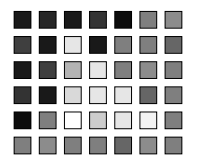
\includegraphics[width=0.55\textwidth]{gambar/gambar_1-A.png}
    \caption{Sebuah gambar}
  \end{subfigure}%
  \begin{subfigure}{.5\textwidth}
    \centering{}
    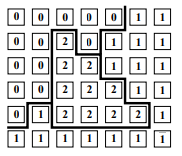
\includegraphics[width=0.55\textwidth]{gambar/gambar_1-B.png}
    \caption{Sebuah label}
  \end{subfigure}  
\caption{
    Contoh pelabelan gambar. citra (a) adalah himpunan piksel P dengan intensitas teramati Ip untuk setiap \(p \in P.\) Pelabelan L yang ditunjukkan 
    pada (b) memberikan beberapa label Lp ∈ {0, 1, 2} untuk setiap piksel \(p \in P.\) 
    } (\cite{Boykov:2004})
\label{img:pelabelan_citra}
\end{figure}


Pada gambar ditunjukkan bahwa \emph{graph} dengan tepi berbobot dapat digunakan untuk 
meminimalkan fungsi energi dengan hukuman interaksi linier dalam kasus multi-label. 
Konstruksi \emph{graph} ini telah diperluas untuk menangani klik cembung dan interaksi 
metrik. Metode yang disebut algoritma ekspans-\(\alpha\) menemukan solusi perkiraan 
dengan menjalankan algoritma \emph{min-cut/max-flow} pada \emph{graph} yang sesuai. 
Pendekatan ini dapat menangani berbagai macam klik, termasuk yang disukai dalam 
aplikasi praktis. Studi terbaru telah mengeksplorasi sifat teoritis konstruksi 
\emph{graph} yang digunakan dalam penglihatan. Sebuah studi mengidentifikasi kondisi 
yang diperlukan dan cukup untuk fungsi energi yang dapat diminimalkan menggunakan 
\emph{graph cut}. Namun, penelitian tersebut hanya berlaku untuk fungsi energi 
dengan variabel biner dan klik ganda atau tripel. Potensi penuh teknik \emph{graph cut} 
dalam kasus multi-label belum sepenuhnya dipahami

Sifat-sifat segmen yang dibuat dengan metode \emph{graph cut} diperiksa dalam 
sebuah penelitian yang disebutkan [3]. Penelitian ini berfokus pada metrik potongan 
yang diterapkan pada kisi \emph{graph} dan menunjukkan bahwa topologi diskrit dari 
\emph{graph cut} dapat meniru ruang metrik Riemannian secara kontinu. Penelitian 
dilakukan yang ada telah menciptakan hubungan antara dua pendekatan umum yang 
digunakan untuk meminimalkan energi: metode \emph{graph cut} kombinatorial 
dan metode geometris yang mengandalkan \emph{set level}.


\subsection{{Latar Belakang Pada Graf}}

Graf berbobot dan berarah, dilambangkan dengan \(G = \langle V, \varepsilon \rangle \) 
terdiri dari kumpulan \emph{node} V dan sisi berarah E yang menghubungkannya. 
\emph{Node} ini biasanya mewakili fitur, seperti piksel atau voxel. Graf juga 
menyertakan beberapa \emph{node} khusus yang dikenal sebagai terminal, yang sesuai 
dengan kemungkinan label yang dapat diberikan ke fitur, khususnya dalam konteks 
penglihatan. Pembahasan ini akan difokuskan pada graf yang hanya memiliki dua terminal.

\begin{figure}[H]
  \centering
    \begin{subfigure}{.5\textwidth}
      \centering{}
      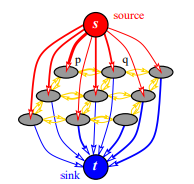
\includegraphics[width=0.55\textwidth]{gambar/graph-A.png}
      \caption{Sebuah graf \(G\)}
    \end{subfigure}%
    \begin{subfigure}{.5\textwidth}
      \centering{}
      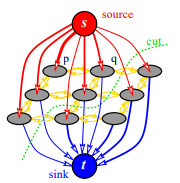
\includegraphics[width=0.55\textwidth]{gambar/cut-A.png}
      \caption{Sebuah potongan (\emph{cut}) \(G\)}
    \end{subfigure}  
  \caption{
    Contoh graf berkapasitas terarah. (\cite{Boykov:2004})
    }
  \label{img:graf_berarah}

\end{figure}

Terminal dalam \emph{graph} dikenal sebagai \emph{source} "s", dan \emph{sink}, "t." Contoh 
sederhana dari \emph{graph} dua terminal ditunjukkan pada Gambar \ref{img:graf_berarah}(a), yang dapat 
digunakan untuk meminimalkan energi Potts pada gambar \(3 x 3\) dengan dua label. 
Sebagian besar metode minimisasi energi dalam penglihatan didasarkan pada \emph{graph} 
grid 2D atau 3D biasa seperti yang ada pada Gambar \ref{img:graf_berarah}(a) karena simpul \emph{graph} biasanya 
mewakili piksel atau voxel gambar biasa. Setiap sisi dalam \emph{graph} memiliki bobot 
atau \emph{cost}, dan \emph{cost} sisi berarah \((p, q)\) mungkin berbeda dari \emph{cost} sisi sebaliknya 
\((q, p)\). Penting untuk dapat menetapkan bobot tepi yang berbeda untuk \((p, q)\) dan 
\((q, p)\) di banyak aplikasi berbasis \emph{graph} dalam penglihatan. \emph{Graph} biasanya terdiri 
dari dua jenis sisi: \emph{n-link} dan \emph{t-link}. \emph{N-link} menghubungkan piksel atau voxel 
yang bertetangga dan merepresentasikan sistem ketetanggaan dalam gambar. \emph{cost} 
\emph{n-link} sesuai dengan penalti untuk diskontinuitas antara piksel, yang berasal dari 
istilah interaksi piksel \(V_{p,q}\) dalam energi (\ref{eq:rumus_energi}). \emph{T-link} menghubungkan piksel 
dengan terminal (label), dan \emph{cost} \emph{t-link} yang menghubungkan piksel dan terminal 
sesuai dengan penalti untuk menetapkan label yang sesuai ke piksel, yang berasal 
dari istilah data \(D_{p}\) dalam energi (\ref{eq:rumus_energi}).

\subsubsection{Permasalahan pada \emph{Min-Cut} dan \emph{Max-Flow}} 

Sebuah \emph{Cut} pada graf dengan dua terminal, dinotasikan sebagai s/t, adalah 
pemisahan \emph{node} dalam graf menjadi dua himpunan bagian yang terpisah dan 
tidak tumpang tindih, S dan T. \emph{Source} (s), termasuk dalam himpunan bagian S, 
dan \emph{sink} (t), termasuk dalam subset T. Pemotongan s/t disebut sebagai \emph{cuts}. 
Contoh potongan ditunjukkan pada gambar \ref{img:graf_berarah} (b).

\begin{figure}[H]
  \centering
    \begin{subfigure}{0.3\textwidth}
      \centering{}
      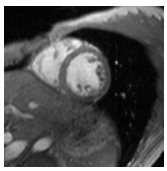
\includegraphics[width=\textwidth]{gambar/gambar-2.png}
      \caption{Gambar Awal}
    \end{subfigure}%
    \begin{subfigure}{0.3\textwidth}
      \centering{}
      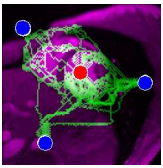
\includegraphics[width=\textwidth]{gambar/gambar-2a.png}
      \caption{\emph{Maximum Flow}}
    \end{subfigure}  
    \begin{subfigure}{0.3\textwidth}
      \centering{}
      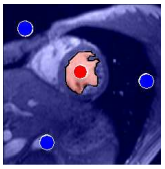
\includegraphics[width=\textwidth]{gambar/gambar-2b.png}
      \caption{\emph{Minimum Cut}}
    \end{subfigure}   
  \caption{
    Contoh (\emph{graph cut})/\emph{flow} dalam konteks segmentasi gambar. 
    (a) menunjukkan \emph{maximum flow} dari s ke t. Faktanya, ini menjenuhkan tepi 
    \emph{graph} yang sesuai dengan batas \emph{minimum cut} di (b). (\cite{Boykov:2004})
    }
    \label{img:contoh_flow}
\end{figure}
Dalam optimasi kombinatorial, \emph{cost} \emph{cut} \(C = {\mathcal{S,T}}\) didefinisikan sebagai 
jumlah \emph{cost} dari tepi batas (p, q) di mana \(p \in S\) dan \(q \in T\) . Perhatikan 
bahwa \emph{cost} \emph{cut} adalah "diarahkan" karena menjumlahkan bobot dari sisi-sisi 
yang diarahkan secara khusus dari \(\mathcal{S}\) ke \(\mathcal{T}\) . Masalah \emph{minimum cut}  pada 
graf adalah menemukan \emph{cut} yang memiliki \emph{cost} minimum di antara semua \emph{cut}. 

Salah satu konsep dasar dalam optimisasi kombinatorial adalah bahwa masalah mencari 
\emph{minimum cut} s/t dapat diselesaikan dengan menentukan \emph{maximum flow} dari 
\emph{source} s ke \emph{sink} t. Secara sederhana, \emph{maximum flow} mewakili 
"jumlah air" maksimum yang dapat diangkut dari sumber ke sumur dengan mempertimbangkan 
tepi graf sebagai pipa yang diarahkan dengan kapasitas yang sama dengan bobot tepinya. 
Menurut teorema Ford dan Fulkerson, \emph{maximum flow} dari s ke t mengisi sekelompok 
tepi di graf yang memisahkan simpul-simpul menjadi dua bagian yang tidak beririsan, 
\({S, T}\), yang sesuai dengan \emph{minimum cut}. Oleh karena itu, masalah 
\emph{minimum cut} dan \emph{maximum flow} adalah setara, dan nilai \emph{maximum flow} 
sama dengan \emph{cost} \emph{minimum cut}. Hubungan "dualitas" antara masalah \emph{maximum flow} 
dan \emph{minimum cut} diilustrasikan pada gambar \ref{img:contoh_flow} dalam konteks segmentasi gambar, 
di mana \emph{maximum flow} yang ditampilkan pada gambar \ref{img:contoh_flow}(a) mengisi 
tepi-tepi pada batas \emph{minimum cut} pada gambar \ref{img:contoh_flow}(b).

Konsep \emph{min-cut} atau \emph{max-flow} pada graf dapat digunakan untuk meminimalkan 
energi dalam pelabelan gambar. Jika kita memiliki gambar 3x3 dan menerapkan \emph{cut} 
s/t padanya, \emph{node} akan dibagi menjadi kelompok terpisah, masing-masing hanya 
berisi satu terminal. Pembagian ini mewakili penugasan piksel ke label. Dengan 
memberikan bobot tepat pada tepian berdasarkan parameter energi, kita dapat mencapai 
energi minimum dengan mencari pemotongan \emph{cost} minimum yang sesuai dengan 
pelabelan energi minimum.

% \subsubsection{Algoritma Standar dalam Optimasi Kombinatorial} \label{bagian:algoritma_standar}

% Fakta penting dalam optimasi kombinatorial adalah adanya algoritma polinomial untuk 
% masalah \emph{min cut/max-flow} pada graf berbobot terarah dengan dua terminal. Sebagian 
% besar algoritma termasuk dalam salah satu dari dua kelompok berikut: metode "\emph{push-relabel}" 
% gaya Goldberg-Tarjan dan algoritma berdasarkan \emph{augmenting path} gaya Ford-Fulkerson.


% Algoritma berbasis \emph{augmenting path} seperti algoritma Dinic bekerja dengan mencari jalur yang tidak jenuh 
% dari sumber ke tujuan dalam suatu graf dan mendorong aliran sepanjang jalur tersebut 
% hingga mencapai aliran maksimum. Algoritma \emph{augmenting path} menyimpan informasi 
% tentang distribusi aliran saat ini \(s \rightarrow t\) di antara tepi-tetapi graf 
% \(\mathcal{G}\) menggunakan graf residual \(\mathcal{G}_{f}\). Topologi 
% \(\mathcal{G}_{f}\) sama dengan \(\mathcal{G}\) tetapi kapasitas tepi di \(\mathcal{G}_{f}\) 
% mencerminkan kapasitas residu di tepi yang sama di \(\mathcal{G}\) dengan jumlah 
% aliran yang sudah ada di tepi tersebut. Pada awalnya, graf residual \( \mathcal{G}_{0} \) 
% tidak memiliki aliran (f=0) dan kapasitas tepi di graf residual \( \mathcal{G}_{0} \) 
% sama dengan kapasitas tepi di \(\mathcal{G}\). Pada setiap iterasi baru, algoritma menemukan 
% jalur \(s \rightarrow t\) terpendek di sepanjang tepi yang tidak jenuh di graf 
% residual \(\mathcal{G}_{f}\). Jika suatu jalur ditemukan, algoritma menambahkannya 
% dengan mendorong aliran maksimum yang mungkin \(df\) yang menjejali setidaknya satu 
% tepi dalam jalur tersebut. Kapasitas residu tepi dalam jalur dikurangi oleh \(df\) 
% sementara kapasitas residu tepi terbalik ditingkatkan oleh \(df\). Setiap penambahan 
% atau \emph{augmentation} eningkatkan total aliran dari sumber ke tujuan, yaitu \(f = f + df\). Aliran maksimum 
% tercapai ketika setiap jalur \(s \rightarrow t\) melintasi setidaknya satu tepi 
% jenuh di graf residual \(\mathcal{G}_{f}\).

% Algoritma Dinic menggunakan pencarian luas pertama untuk menemukan jalur terpendek
% dari \(s\) ke \(t\) pada graf residual \(\mathcal{G}_{f}\). Setelah semua jalur terpendek dengan panjang 
% tetap \(k\) jenuh, algoritma memulai pencarian pertama lebar untuk \(s \rightarrow t\) jalur dengan 
% panjang \(k + 1\) dari awal. Perhatikan bahwa penggunaan jalur terpendek merupakan 
% faktor penting yang meningkatkan kompleksitas waktu berjalan teoretis untuk algoritma 
% berdasarkan jalur augmentasi. Kompleksitas running time kasus terburuk untuk algoritma 
% Dinic adalah \(O(mn^2 )\) di mana \(n\) adalah jumlah \emph{node} dan \(m\) adalah jumlah sisi dalam graf.

% Algoritma \emph{push-relabel} berbeda dengan metode \emph{augmenting path} karena 
% tidak berfokus pada menjaga \emph{flow} yang valid selama operasi. Sebaliknya, mereka 
% mencatat \emph{node} aktif dengan kelebihan \emph{flow} positif dan memberikan perkiraan batas 
% bawah jarak ke \emph{sink} melalui edge yang belum jenuh. Tujuannya adalah untuk mendorong 
% \emph{flow} yang berlebihan ke \emph{node} dengan perkiraan jarak yang lebih kecil ke sink. 
% Operasi push biasanya diterapkan pada \emph{node} aktif dengan jarak terbesar atau berdasarkan 
% strategi seleksi FIFO. Saat operasi push jenuh, jarak (label) meningkat secara progresif. 
% \emph{Flow} yang tidak dapat disampaikan akhirnya dikembalikan ke \emph{source}.


\subsection{{Algoritma \emph{Mincut/Max-Flow} Terbaru}}


Untuk meningkatkan performa empiris teknik augmenting path standar pada graf 
dalam \emph{computer vision}, \cite{Boykov:2004} mengembangkan algoritma baru. Biasanya, 
metode \emph{augmenting path} memulai pencarian lebar baru untuk jalur \(s \rightarrow t\) 
segera setelah semua jalur dari panjang tertentu habis. Namun, membangun pohon 
pencarian lebar untuk graf dalam \emph{computer vision} melibatkan pemindaian sebagian 
besar piksel gambar, sehingga menjadi operasi yang mahal jika dilakukan terlalu 
sering. Eksperimen dengan data nyata dalam \emph{computer vision} mengonfirmasi bahwa 
membangun kembali pohon pencarian menghasilkan kinerja yang buruk dari teknik 
\emph{augmenting path} standar. Untuk mengatasi masalah ini, \cite{Boykov:2004} 
mengembangkan beberapa ide yang meningkatkan performa empiris teknik \emph{augmenting path} 
pada graf dalam \emph{computer vision}.


\begin{figure}[H]
  \centering
  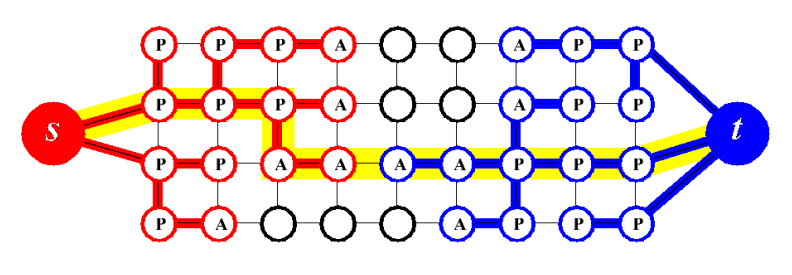
\includegraphics[width=0.8\textwidth]{gambar/gambar-3.png}
  \caption{
    Contoh pencarian pohon \(S\) (\emph{node} merah) dan \(T\) (\emph{node} biru) (\cite{Boykov:2004})
    }
  \label{img:contoh_pencarian_pohon}
\end{figure}

Algoritma min-cut/max-flow baru yang disajikan di sini termasuk dalam kelompok 
algoritma berdasarkan \emph{augmenting path}. Seperti algoritma Dinic, algoritma 
yang dibuat oleh \cite{Boykov:2004} juga membuat pohon pencarian untuk mendeteksi 
jalur pembesaran. Namun, membuat dua pohon pencarian, satu dari \emph{source} dan satu 
lagi dari \emph{sink}. Menggunakan kembali pohon-pohon ini dan tidak membuatnya 
dari awal setiap kali. Salah satu kelemahan pendekatan algoritma ini adalah jalur 
pembesaran yang ditemukan tidak selalu merupakan jalur pembesaran terpendek, sehingga 
kompleksitas waktu untuk menemukan jalur pembesaran terpendek tidak lagi valid. 
Jumlah maksimum penambahan yang dapat dilakukan oleh algoritma, dibatasi oleh 
biaya \emph{minimum cut} \(|C|\), sehingga kompleksitas waktu terburuknya adalah
\(O(mn^2 |C|)\).

\subsubsection{Penjelasan Algoritma} 

\cite{Boykov:2004} mempertahankan dua pohon pencarian yang tidak tumpang tindih 
\(S\) dan \(T\) dengan akar pada \emph{source} s dan \emph{sink} t, secara berurutan. 
Pada pohon S semua sisi dari setiap \emph{node} induk ke anaknya tidak jenuh, sedangkan 
pada pohon T sisi dari anak ke induknya tidak jenuh. \emph{node} yang tidak ada di S atau T 
disebut "bebas".

\begin{equation} \label{eq:status_node}
  S \subset V, s \in S, T \subset V, t \in T, S \cap T = 0
\end{equation} 

\emph{Node} dalam pohon pencarian \(S\) dan \(T\) dapat berupa "aktif" atau "pasif". \emph{node} 
aktif mewakili batas luar di setiap pohon sedangkan \emph{node} pasif adalah internal. 
Intinya adalah \emph{node} aktif memungkinkan pohon untuk "tumbuh" dengan memperoleh 
anak baru (sepanjang tepi yang tidak jenuh) dari sekumpulan \emph{node} bebas. 
\emph{node} pasif tidak dapat tumbuh karena sepenuhnya diblokir oleh \emph{node} 
lain dari pohon yang sama. Penting juga bahwa \emph{node} aktif dapat bersentuhan dengan 
\emph{node} dari pohon lain. Jalur augmentasi ditemukan segera setelah \emph{node} aktif 
di salah satu pohon mendeteksi \emph{node} tetangga yang dimiliki oleh pohon lainnya.


Algoritma secara iteratif mengulangi tiga tahap berikut:
\begin{itemize}
    \item Tahap “pertumbuhan atau (\emph{growth})”: cari pohon \(S\) dan \(T\) tumbuh hingga bersinggungan memberikan jalur \(s \rightarrow t\)  
    \item Tahap "augmentasi atau (\emph{augmentation})": jalur yang ditemukan ditambah, pohon pencarian dipecah menjadi hutan
    \item Tahap “adopsi atau (\emph{adoption})”: pohon \(S\) dan \(T\) dipulihkan.
\end{itemize}

% Pada tahap pertumbuhan atau (\emph{growth}), pohon pencarian berkembang dan \emph{node} 
% aktif mengeksplorasi tepi yang tidak jenuh dan memperoleh anak baru dari himpunan 
% \emph{node} bebas. Anak yang baru diperoleh menjadi anggota aktif dari pohon pencarian 
% yang sesuai. Ketika semua tetangga dari \emph{node} aktif telah dijelajahi, \emph{node} 
% aktif menjadi pasif. Tahap pertumbuhan berakhir ketika \emph{node} aktif menemukan 
% \emph{node} tetangga yang termasuk dalam pohon pencarian yang berlawanan, menandakan 
% bahwa telah ditemukan jalur dari \emph{source} ke \emph{sink}.

Pada tahap pertumbuhan (\emph{growth}), pohon pencarian berkembang dengan \emph{node} 
aktif mengeksplorasi tepi yang belum terjenuh dan mendapatkan anak baru dari himpunan 
\emph{node} bebas. Anak-anak baru ini menjadi bagian aktif dari pohon pencarian yang 
sesuai. Ketika semua tetangga dari \emph{node} aktif telah dijelajahi, status \emph{node} aktif 
berubah menjadi pasif. Tahap pertumbuhan berakhir ketika \emph{node} aktif menemukan 
tetangga yang sudah ada dalam pohon pencarian lawan, menunjukkan penemuan jalur dari 
\emph{source} ke \emph{sink}.

% Pada tahap augmentasi, jalur yang ditemukan pada tahap pertumbuhan ditambah dengan 
% mendorong aliran terbesar yang mungkin melalui jalur tersebut. Hal ini dapat 
% menyebabkan beberapa tepi menjadi jenuh, sehingga beberapa \emph{node} dalam pohon 
% \(S\) dan \(T\) menjadi "\emph{orphans}" karena tautan mereka ke induknya tidak lagi 
% valid. Tahap augmentasi juga dapat membagi pohon \(S\) dan \(T\) menjadi hutan.
% Namun, pada tahap adopsi atau (\emph{adoption}), tujuannya adalah untuk mengembalikan 
% struktur satu-pohon ke dalam himpunan \(S\) dan \(T\) dengan akar di \emph{source} 
% dan \emph{sink}. Ini dicapai dengan mencari induk baru yang valid untuk setiap 
% \emph{orphans} dalam himpunan yang sama, terhubung melalui tepi yang tidak jenuh. Jika 
% tidak ditemukan induk yang memenuhi syarat, \emph{orphans} dihapus dari \(S\) atau \(T\) 
% dan menjadi \emph{node} bebas, dan semua anak yang sebelumnya menjadi \emph{orphans}.

Pada tahap augmentasi, jalur yang ditemukan pada tahap pertumbuhan ditingkatkan 
dengan mengalirkan aliran maksimum melalui jalur tersebut. Ini bisa membuat beberapa 
tepi menjadi jenuh, mengakibatkan beberapa \emph{node} dalam himpunan \(S\) dan \(T\) menjadi 
\emph{"orphans"} karena tautan induk mereka tidak lagi valid. Tahap augmentasi juga bisa 
memisahkan pohon \(S\) dan \(T\) menjadi hutan.

Pada tahap adopsi, tujuannya adalah mengembalikan struktur satu-pohon ke dalam himpunan 
\(S\) dan \(T\) dengan akar di \emph{source} dan \emph{sink}. Ini dilakukan dengan mencari induk 
baru yang valid untuk setiap \emph{"orphans"} dalam himpunan yang sama, terhubung melalui 
tepi yang tidak jenuh. Jika tidak ditemukan induk yang memenuhi syarat, \emph{"orphans"} 
dihapus dari \(S\) atau \(T\), menjadi \emph{node} bebas, dan semua anak yang sebelumnya 
menjadi \emph{"orphans"}.

% Tahap adopsi atau \emph{adoption} terus berlanjut sampai semua \emph{orphans} telah menemukan induk 
% baru yang valid atau telah menjadi \emph{node} bebas. Proses ini akan memperkecil ukuran 
% \emph{set} \(S\) dan \(T\). Setelah tahap adopsi selesai, algoritma kembali ke tahap pertumbuhan. 
% Algoritma berakhir saat tidak ada lagi \emph{node} aktif tersisa dan pohon pencarian \(S\) dan \(T\) 
% terpisah oleh tepi yang jenuh, menunjukkan bahwa aliran maksimum telah dicapai. 
% Potongan minimum dapat ditentukan dengan menetapkan \(S\) dan \(T\) pada pohon yang sesuai.

Tahap adopsi \emph{(adoption)} berlanjut sampai semua \emph{"orphans"} telah menemukan 
induk baru yang valid atau telah menjadi \emph{node} bebas. Ini mengakibatkan pengurangan 
ukuran set \(S\) dan \(T\). Setelah tahap adopsi selesai, algoritma kembali ke tahap 
pertumbuhan. Algoritma berakhir saat tidak ada \emph{node} aktif yang tersisa dan pohon 
pencarian \(S\) dan \(T\) terisolasi oleh tepi yang jenuh, menunjukkan pencapaian 
aliran maksimum. Potongan minimum dapat ditentukan dengan menetapkan \(S\) dan \(T\) 
pada pohon yang sesuai.

\subsubsection{Implementasi Lebih Lanjut} 

Asumsikan bahwa kita memiliki graf berarah \(\mathcal{G = hV, Ei}\). Untuk setiap algoritma 
\emph{augmenting path}, kita akan mempertahankan aliran \(f\) dan graf residual \(Gf\) 
(lihat Bagian 2.1.2.2). Menyimpan daftar semua \emph{node} aktif, \(A\), dan semua \emph{orphans}, \(O\). 
Struktur umum algoritma adalah:

\begin{lstlisting} [label={pseudo:1.0}]
  initialize: (S = {s}, T = {t}, A = {s, t}, O = Ø)
  while true
      grow S or T to find an augmenting path P from s to t
      if P = Ø terminate
      augment on P
      adopt orphans
  end while  
\end{lstlisting}

Rincian tahap pertumbuhan, augmentasi, dan adopsi dijelaskan di bawah ini. Lebih 
mudah untuk menyimpan muatan dari pohon pencarian \(S\) dan \(T\) melalui \(flag\) \emph{TREE(p)} 
yang menunjukkan afiliasi dari setiap \emph{node} p sehingga

\begin{equation} \label{eq:searchtree_awal}
  TREE(p) =  \Biggl\{\begin{matrix}
    S & if & p & \in & S\\
    T & if & p & \in & T\\
    $\O$ & if & p & is & free
    \end{matrix}
\end{equation}

Jika \emph{node} p milik salah satu pohon pencarian maka informasi tentang induknya 
akan disimpan sebagai \(PARENT(p)\). Akar pohon pencarian (\emph{source} dan \emph{sink}), 
\emph{orphans}, dan semua \emph{node} bebas tidak memiliki orang tua, 
t.e. \emph{PARENT(p)} = Ø. Notasi \(tree\textunderscore cap(p \rightarrow q)\) 
untuk mendeskripsikan kapasitas residual dari salah satu sisi \((p, q)\) jika \(TREE(p) = S\) 
atau sisi \((q, p)\) jika \(TREE(p) = T\). Sisi-sisi ini harus tidak jenuh agar 
\emph{node} p menjadi orangtua yang valid dari anaknya q tergantung pada pohon pencarian.

\paragraph{Fase \emph{Growth}} \label{fase_growth}

Pada tahap ini node aktif memperoleh anak baru dari satu set node bebas.

\begin{lstlisting}
  while A $\neq$ Ø
    pick an active node $p \in A$
    for every neighbor q such that $tree\textunderscore cap(p \rightarrow q)$ > 0
    if $TREE(q) =$ Ø then add q to search tree 
    as an active node:
    $TREE(q) \neq TREE(p), PARENT(q) \neq p, A \neq A \cup \{q\}$
    if $TREE(q) \neq$ Ø and $TREE(q) \neq TREE(p)$ 
    return $P = PATH_{s \rightarrow t}$
    end for
    remove p from A
  end while
  return P = Ø
\end{lstlisting}


\paragraph{Fase \emph{Augmentation}} \label{fase_augmentation}

Input untuk tahap ini adalah jalur P dari s ke t. Perhatikan bahwa himpunan anak 
yatim kosong pada awal tahap, tetapi mungkin ada beberapa \emph{orphans} pada akhirnya 
karena setidaknya satu sisi di P menjadi jenuh.

\begin{lstlisting}
  find the bottleneck capacity $\Delta$ on P
  update the residual graph by pushing flow $\Delta$ through P
  for each \emph{edge} $(p, q)$ in P that becomes saturated
    if $TREE(p) = TREE(q)$ = S 
      then set $PARENT(q)$ := Ø and $O := O \cup {q}$
    if $TREE(p) = TREE(q)$ = T 
      then set $PARENT(p)$ := Ø and $O := O \cup {p}$
  end for
\end{lstlisting}


\paragraph{Fase \emph{Adoption}} \label{fase_adoption}

Selama tahap ini semua \emph{node} \emph{orphans} di O diproses sampai O menjadi kosong. 
Setiap \emph{node} p sedang diproses mencoba menemukan induk baru yang valid di dalam pohon 
pencarian yang sama; jika berhasil, p tetap berada di pohon tetapi dengan induk baru, 
jika tidak, ia menjadi \emph{node} bebas dan semua anaknya ditambahkan ke O.

\begin{lstlisting}
  while O $\neq$ Ø  
    pick an orphan node $p \in O$ and remove it from O
    process p
  end while
\end{lstlisting}

Operasi \emph{"proses p"} terdiri dari langkah-langkah berikut. Pertama kita mencoba mencari 
induk valid baru untuk \(p\) di antara tetangganya. Induk \(q\) yang valid harus memenuhi: 
\(TREE(q) = TREE(p)\), \(tree\textunderscore cap(q \rightarrow p) > 0\), dan “origin” 
dari \(q\) harus berupa \emph{source} atau c \emph{sink}. Perhatikan bahwa kondisi terakhir 
diperlukan karena selama tahap adopsi beberapa \emph{node} dalam pohon pencarian \(S\) atau \(T\) 
mungkin berasal dari \emph{orphans}. Jika \emph{node} \(p\) menemukan induk baru yang valid 
\(q\) maka kita atur \(PARENT(p) = q\). Dalam hal ini \(p\) tetap berada di pohon pencariannya 
dan status aktif (atau pasif) p tetap tidak berubah. 

Jika \(p\) tidak menemukan induk yang valid maka \(p\) menjadi \emph{node} bebas dan operasi 
berikut dilakukan:

\begin{itemize}
  \item Memindai semua tetangga q dari p sehingga TREE(q) = TREE(p):  
  \begin{itemize}
    \item jika \(tree\textunderscore cap(q \rightarrow p) > 0\) tambahkan q kepada set A yang aktif
    \item jika \(PARENT(q) = p\) tambahkan q kepada set \emph{orphans} O dan set \(PARENT(q) :=\) Ø
  \end{itemize}
  \item \(TREE(p) :=\) Ø, \(A := A - \{p\}\)
\end{itemize}

Perhatikan bahwa ketika \(p\) menjadi bebas, semua tetangganya yang terhubung melalui 
tepi yang tidak jenuh harus menjadi aktif. Mungkin saja beberapa tetangga \(q\) tidak 
memenuhi syarat sebagai orang tua yang valid selama tahap adopsi karena tidak berasal 
dari sumber atau sink. Namun, \emph{node} ini bisa menjadi induk yang valid setelah 
tahap adopsi selesai. Pada titik ini \(q\) harus berstatus aktif karena terletak di 
sebelah \emph{node} bebas \(p\).


\section{Segmentasi Citra dengan Algoritma \emph{GrabCut}}

% \cite{Rother:2004} melakukan penelitian mengenai segmentasi gambar dengan memanfaatkan 
% citra gambar, menyatakan bahwa alat segmentasi gambar klasik menggunakan salah satu 
% informasi tekstur (warna), misalnya. \emph{Magic Wand}, atau informasi tepi (kontras), 
% misalnya \emph{Intelligent Scissors}. \cite{Rother:2004} melakukan pendekatan yang didasarkan 
% pada pengoptimalan dengan \emph{GraphCut} telah dikembangkan yang berhasil menggabungkan 
% kedua jenis informasi tersebut.

% Ekstraksi interaktif dari objek latar depan dalam lingkungan kompleks yang latar 
% belakangnya tidak dapat dikurangkan dengan mudah. Tujuan dari algoritma ini adalah 
% untuk menghasilkan pemisahan objek dari latar belakang yang berkualitas tinggi, 
% sambil hanya memerlukan sedikit masukan dari pengguna. Output dari algoritma ini 
% adalah \emph{alpha-matte}, yang menunjukkan proporsi \emph{foreground} dan \emph{background} pada 
% setiap piksel.  Algoritma ini bertujuan untuk mencapai segmentasi objek yang akurat, 
% nilai alpha yang meyakinkan yang memperhitungkan blur, piksel campuran, dan transparansi, 
% serta warna \emph{foreground} yang bersih dan tidak terpengaruh oleh bleeding warna 
% dari latar belakang asli. Jumlah interaksi yang dibutuhkan dari pengguna dapat 
% bervariasi mulai dari mengedit piksel individu hingga hanya menandai beberapa lokasi 
% \emph{foreground} atau \emph{background}. 

Penelitian oleh \cite{Rother:2004} mengenai segmentasi gambar memanfaatkan citra 
dan menyatakan bahwa alat segmentasi gambar klasik menggunakan informasi tekstur 
(misalnya, warna) seperti \emph{Magic Wand}, atau informasi tepi (misalnya 
\emph{Intelligent Scissors}). Pendekatan yang digunakan oleh \cite{Rother:2004} 
berbasis pengoptimalan dengan \emph{GraphCut} dan berhasil menggabungkan kedua jenis 
informasi tersebut.

Tujuan algoritma ini adalah memisahkan objek dari latar belakang dalam lingkungan 
kompleks tanpa memerlukan banyak masukan pengguna. Hasilnya berupa alpha-matte yang 
menunjukkan proporsi \emph{foreground} dan \emph{background} pada setiap piksel. Algoritma ini 
bertujuan untuk memberikan segmentasi objek yang akurat, nilai alpha yang memperhitungkan 
blur, piksel campuran, transparansi, dan warna \emph{foreground} yang bersih tanpa 
terpengaruh oleh warna latar belakang. Jumlah interaksi pengguna dapat bervariasi, 
mulai dari mengedit piksel hingga menandai lokasi \emph{foreground} atau \emph{background}.

\subsection{{Sistem yang Diusulkan : \emph{GrabCut}}}

% Sebuah alat pemotongan gambar yang baik seharusnya dapat menghasilkan nilai alpha 
% yang halus di seluruh wilayah inferensi dari trimap, tanpa memberlakukan batasan 
% keras yang membatasi nilai alpha menjadi hanya 0 atau 1. Hal ini akan memungkinkan 
% untuk menangani secara otomatis masalah seperti asap, rambut, dan pohon. Namun, ini 
% menunjukkan bahwa teknik yang dirancang untuk memecahkan masalah 
% pemotongan gambar secara umum hanya efektif ketika terdapat cukup pemisahan antara 
% distribusi warna \emph{foreground} dan \emph{background}.

% Pertama kita memperoleh segmentasi “keras” menggunakan \emph{Graph Cut} iteratif. 
% Ini diikuti dengan \emph{matting} batas (bagian 4) di mana nilai \emph{alpha} dihitung dalam 
% jalur sempit di sekitar batas segmentasi keras. Terakhir, transparansi penuh, selain 
% di perbatasan, tidak ditangani oleh \emph{GrabCut} . Itu bisa dicapai namun menggunakan 
% \emph{matting brush} dan, ini bekerja dengan baik di area yang cukup bebas.

% Kebaruan pendekatan yang dilakukan Boykov pertama-tama terletak pada penanganan segmentasi. \cite{Boykov:2004} 
% telah membuat dua peningkatan pada mekanisme \emph{Graph Cut}: "estimasi iteratif" 
% dan "pelabelan tidak lengkap" yang memungkinkan tingkat interaksi pengguna yang 
% sangat berkurang untuk kualitas hasil tertentu (gambar \ref{img:2.5}(f)). Hal ini memungkinkan 
% \emph{GrabCut} untuk memberi beban ringan pada pengguna, yang interaksinya hanya 
% terdiri dari menyeret persegi panjang di sekitar objek yang diinginkan. Dengan 
% demikian, pengguna menunjukkan wilayah latar belakang, dan bebas dari kebutuhan 
% untuk menandai wilayah latar depan. Mereka juga telah mengembangkan mekanisme 
% baru untuk komputasi \emph{alpha}, yang digunakan untuk \emph{border matting}, di mana nilai 
% \emph{alpha} diatur untuk mengurangi artefak yang terlihat.

Alat pemotongan gambar yang baik harus menghasilkan nilai alpha yang halus di seluruh 
wilayah inferensi trimap, tanpa batasan keras 0 atau 1, untuk menangani masalah seperti asap, 
rambut, dan pohon. Teknik pemotongan gambar umumnya efektif saat ada pemisahan 
yang jelas antara distribusi warna \emph{foreground} dan \emph{background}.

Langkah pertama adalah segmentasi "keras" menggunakan \emph{Graph Cut} iteratif. 
Kemudian dilakukan matting batas di sekitar segmentasi keras, di mana nilai alpha 
dihitung dalam jalur sempit. Namun, GrabCut tidak menangani transparansi penuh 
selain di perbatasan, yang dapat dicapai dengan matting brush dalam area yang cukup bebas.

Pendekatan Boykov memperkenalkan peningkatan pada mekanisme \emph{Graph Cut}. Ini mencakup 
"estimasi iteratif" dan "pelabelan tidak lengkap" yang mengurangi interaksi pengguna. 
GrabCut memberikan kemudahan interaksi bagi pengguna dengan hanya menarik persegi 
panjang di sekitar objek. Mereka juga mengembangkan mekanisme baru untuk menghitung 
alpha dalam \emph{border matting} guna mengurangi artefak.


\subsection{{Segmentasi gambar dengan \emph{graph cut}}}

Segmentasi citra monokrom, diberi trimap awal T. Citra merupakan \emph{array} 
\(\textbf{z} = (z_{1},...,z_{n},...,z_{N})\) dengan nilai keabuan, diindeks dengan indeks (tunggal) n. 
Segmentasi gambar diekspresikan sebagai susunan nilai “opasitas” 
\(\alpha = (\alpha_{1},...,\alpha_{N})\) pada setiap piksel. Umumnya \( 0 \leq \alpha_{n} \leq 1\), 
tetapi untuk segmentasi keras \(\alpha_{n} \in {0,1}\), dengan 0 untuk latar belakang 
dan 1 untuk latar depan. Parameter \(\underline{\theta}\) menggambarkan distribusi 
tingkat keabuan latar depan dan latar belakang, dan terdiri dari histogram nilai 
keabuan: 

\begin{equation} \label{eq:2.4}
  \underline{\theta} = \{h(z;\alpha), \alpha = 0,1\}
\end{equation} 
dimana,
\begin{conditions}
  \theta & Distribusi tingkat keabuan dari gambar citra\\
  \alpha & Nilai alpha tiap piksel 1 untuk \emph{foreground} dan 0 untuk \emph{background}\\
  h & Histogram tingkat keabuan
\end{conditions}

satu untuk latar belakang dan satu untuk latar depan. Histogram dirakit langsung 
dari piksel berlabel dari masing-masing wilayah trimap \(T_{B},T_{F}\) . (Histogram dinormalisasi 
untuk dijumlahkan menjadi 1 pada rentang tingkat abu-abu: \(\int_{z} h(z;\alpha) = 1\).) Tugas 
segmentasi adalah menyimpulkan variabel opasitas yang tidak diketahui \(\alpha\) dari data 
gambar yang diberikan z dan model \(\theta\).

\subsubsection{{Segmentasi dengan \emph{energy minimisation}}}

Fungsi energi \textbf{E} didefinisikan pada persamaan \ref{eq:rumus_energi} yang dijelaskan oleh \cite{Boykov:2004} 
sehingga minimumnya harus sesuai dengan segmentasi yang baik, dalam arti bahwa ia dipandu baik oleh histogram 
tingkat abu-abu latar depan dan latar belakang yang di amati dan bahwa opasitasnya 
"koheren", yang mencerminkan kecenderungan soliditas objek. \cite{Rother:2004} 
menuliskan kembali energi "Gibbs" dalam bentuk:


\begin{equation} \label{eq:2.5}
  E(\underline{\alpha}, \underline{\theta}, \textbf{z}) = U(\underline{\alpha}, 
  \underline{\theta}, \textbf{z}) + V (\underline{\alpha}, \textbf{z})
\end{equation} 

dimana,
\begin{conditions}
  E & \emph{Cost Function} atau Rumus Energi \\
  U(\underline{\alpha}, \underline{\theta}, \textbf{z}) & Data penalti, seperti pada rumus \ref{eq:rumus_energi}\\
  V (\underline{\alpha}, \textbf{z}) & Interaksi potensial yaitu diskontinuitas antar piksel\\
  \textbf{z} & Nilai warna tiap piksel pada citra digital
  % \underline{\theta} & Model distribusi keabua 
\end{conditions}

Istilah data \(U\) mengevaluasi kecocokan distribusi opasitas \(\underline{\alpha}\) 
dengan data \textbf{z}, mengingat model histogram \(\underline{\theta}\), dan didefinisikan sebagai:

\begin{equation} \label{eq:2.6}
  U(\underline{\alpha}, \underline{\theta}, \textbf{z}) = \sum_{n} - \log h(z_{n};\alpha_{n}) 
\end{equation} 

dimana,
\begin{conditions}
  E & \emph{Cost Function} atau Rumus Energi \\
  U(\underline{\alpha}, \underline{\theta}, \textbf{z}) & Data penalti, seperti pada rumus \ref{eq:rumus_energi}\\
  % \underline{\alpha} & Nilai alpha \\
  % \underline{\theta} & Model distribusi keabua 
\end{conditions}

Istilah \emph{smoothness} dapat dituliskan sebagai :

\begin{equation} \label{eq:smoothness}
  V (\underline{\alpha}, \textbf{z}) = \gamma \sum_{(m,n) \in \textbf{C}} dis(m,n)^{-1}
  [\alpha_{n} \neq \alpha_{m}]exp - \beta(z_{m} - z_{n})^2
\end{equation} 

dimana,
\begin{conditions}
  E & \emph{Cost Function} atau Rumus Energi \\
  V (\underline{\alpha}, \textbf{z}) & Interaksi potensial yaitu diskontinuitas antar piksel\\
  \gamma & niai gamma \\
  m & Suatu piksel \\
  n & Tetangga dari piksel m \\
  \beta(z_{m} - z_{n})^2 & \emph{Beta smoothness}
\end{conditions}

di mana \([\phi]\) menunjukkan fungsi indikator yang mengambil nilai 0,1 untuk predikat 
\(\phi\), C adalah himpunan pasangan piksel tetangga, dan \(dis(\cdot)\) adalah jarak Euclidean 
piksel tetangga. Energi ini mendorong koherensi di wilayah dengan tingkat abu-abu 
yang serupa. Dalam praktiknya, hasil yang baik diperoleh dengan mendefinisikan 
piksel sebagai tetangga jika berdekatan baik secara horizontal/vertikal maupun 
diagonal (konektivitas 8 arah). Ketika konstanta \(\beta = 0\), istilah kehalusan 
hanyalah Ising sebelumnya yang terkenal, mendorong kehalusan di mana-mana, hingga 
tingkat yang ditentukan oleh konstanta \(\gamma\). Namun telah ditunjukkan bahwa 
jauh lebih efektif untuk mengatur \(\beta > 0\) karena hal ini mengurangi kecenderungan 
kehalusan di daerah dengan kontras tinggi. Konstanta \(\beta\) dipilih menjadi :

\begin{equation} \label{eq:2.8}
  \beta = \Bigl( 2 \bigl \langle (z_{m} - z_{n})^2 \bigl \rangle \Bigr)^{-1}
\end{equation} 

di mana \(\langle(\cdot)\rangle\) menunjukkan harapan atas sampel gambar. Pilihan 
\(\beta\) ini memastikan bahwa suku eksponensial dalam \ref{eq:smoothness} beralih dengan 
tepat antara kontras tinggi dan rendah. Konstanta \(\gamma\) diperoleh sebesar 50 
dengan mengoptimalkan kinerja terhadap kebenaran dasar melalui satu set pelatihan 
yang terdiri dari 15 gambar. Ini terbukti menjadi pengaturan serbaguna untuk berbagai 
macam gambar. Sekarang setelah model energi didefinisikan sepenuhnya, segmentasi 
dapat diperkirakan sebagai minimum global:

\begin{equation} \label{eq:2.9}
 \hat{\underline{\alpha}}  = arg \min_{\underline{\alpha}} \textbf{E}(\alpha,\theta).
\end{equation} 

Algoritma pemotongan minimum standar digunakan untuk minimisasi. Ini menjadi dasar 
bagi segmentasi keras, yang kemudian mengembangkan tiga perubahan untuk algoritma 
segmentasi dalam GrabCut. Pertama, model gambar monokrom digantikan oleh Model 
Campuran Gaussian (GMM) untuk warna. Kedua, estimasi \emph{one-shot minimum cut} 
diganti dengan prosedur iteratif lebih kuat yang bergantian antara estimasi dan 
pembelajaran parameter. Ketiga, permintaan pengguna interaktif dilemahkan, memungkinkan 
pelabelan yang tidak lengkap - pengguna hanya menentukan \(T_{B}\) untuk trimap, 
dengan cara menempatkan bentuk di sekitar objek.

\begin{figure}[H]
  \centering
    \begin{subfigure}{0.3\textwidth}
      \centering{}
      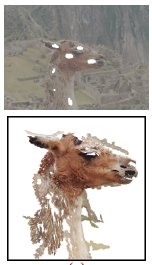
\includegraphics[width=\textwidth]{gambar/gambar-2_5(a).png}
      \caption{\emph{Magic Wand}}
    \end{subfigure}%
    \begin{subfigure}{0.3\textwidth}
      \centering{}
      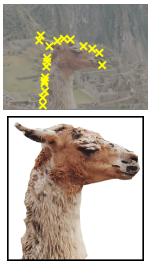
\includegraphics[width=\textwidth]{gambar/gambar-2_5(b).png}
      \caption{\emph{Intelligent Scissors}}
    \end{subfigure}  
    \begin{subfigure}{0.3\textwidth}
      \centering{}
      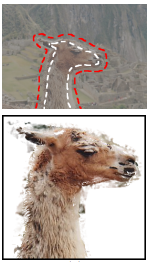
\includegraphics[width=\textwidth]{gambar/gambar-2_5(c).png}
      \caption{\emph{Bayes Matte}}
    \end{subfigure}  
    \begin{subfigure}{0.3\textwidth}
      \centering{}
      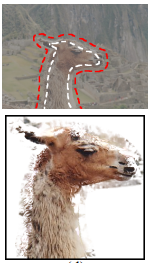
\includegraphics[width=\textwidth]{gambar/gambar-2_5(d).png}
      \caption{\emph{Knockout 2}}
    \end{subfigure}  
    \begin{subfigure}{0.3\textwidth}
      \centering{}
      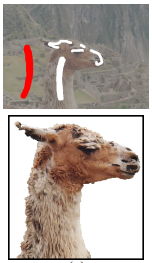
\includegraphics[width=\textwidth]{gambar/gambar-2_5(e).png}
      \caption{\emph{GraphCut}}
    \end{subfigure}   
    \begin{subfigure}{0.3\textwidth}
      \centering{}
      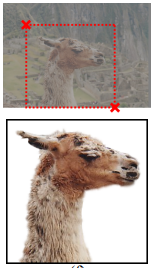
\includegraphics[width=\textwidth]{gambar/gambar-2_5(f).png}
      \caption{\emph{GrabCut}}
    \end{subfigure}  
  \caption{
    Perbandingan beberapa \emph{matting tools} dan segmentasi. (\cite{Rother:2004})
    }
  \label{img:2.5}
\end{figure}


\subsection{{Segmentasi gambar dengan algoritma \emph{GrabCut}}}

\subsubsection{{Model Pendataan Warna}}

Gambar yang ada saat ini terdiri dari piksel \(z_{n}\) dalam ruang warna RGB. 
Karena tidak praktis untuk membuat histogram ruang warna yang memadai, untuk itu 
maka digunakan GMM. Setiap nilai GMM yaitu satu untuk latar belakang dan satu untuk 
latar depan, dianggap sebagai \emph{Gaussian Mixture} penuh dengan komponen K 
(biasanya K = 5). Untuk menangani GMM dengan baik, dalam kerangka optimisasi, vektor 
tambahan \(\textbf{k} = \{k_{1},...,k_{n},...,k_{N}\}\) diperkenalkan, dengan 
\(k_{n} \in \{1,...K\}\) , menetapkan, untuk setiap piksel, komponen GMM unik, satu 
komponen baik dari latar belakang atau model latar depan, menurut \( \alpha n = 0\) 
atau \(1^1\) .


Energi Gibbs untuk segmentasi sekarang menjadi 

\begin{equation} \label{eq:rumus_energi0}
  E(\alpha,k,\theta, z) = U(\alpha,k,\theta, z) + V(\alpha, z)
\end{equation} 

bergantung juga pada variabel komponen GMM k . Istilah data U sekarang didefinisikan, 
dengan mempertimbangkan model GMM warna, sebagai 

\begin{equation} \label{eq:rumus_energi1}
  U(\alpha,k,\theta, z) =  \sum_{n} D(\alpha_{n}, k_{n},\theta,z_{n}),
\end{equation}  

di mana 

\begin{equation} \label{eq:rumus_D}
  D(\alpha n, k_{n} ,\theta,z_{n}) = - \log p(z_{n} | \alpha n, k_{n},\theta) - log \pi(\alpha_n, k_{n})
\end{equation}

yang mana \(p(\cdot)\)  adalah distribusi probabilitas Gaussian, dan \(\pi(\cdot)\) adalah 
koefisien bobot campuran, sehingga : 

\begin{multline} \label{eq:rumus_energi2}
      D(\alpha_{n}, k_{n},\theta,z_{n}) = - log \pi(\alpha_{n}, k_{n}) + \frac{1}{2} logdet \Sigma(\alpha_{n}, k_{n}) \\
      + \frac{1}{2} [z_{n} - \mu (\alpha_{n}, k_{n})]^T \Sigma(\alpha_{n}, k_{n})^{-1} [z_{n} -  \mu (\alpha n, k_{n})]    
\end{multline}

Oleh karena itu, parameter model sekarang adalah 

\begin{equation} \label{eq:rumus_energi3}
  \theta = \{ \pi(\alpha, k), \mu (\alpha, k), \Sigma (\alpha, k), \alpha = 0,1, k = 1...K \},
\end{equation}  

yaitu bobot \(\pi\), berarti \(\mu\) dan kovarians \(\Sigma\) dari komponen \(\mathcal{2K} \)
Gaussian untuk distribusi latar belakang dan latar depan. Istilah kelancaran \(\mathcal{V}\) 
pada dasarnya tidak berubah dari kasus monokrom kecuali bahwa istilah kontras dihitung 
menggunakan jarak \emph{Euclidean} dalam ruang warna: 

\begin{equation} \label{eq:rumus_energi4}
  V(\alpha, z) = \gamma \sum_{(m,n)\in C} [\alpha_{n} \neq \alpha_{m}] \textrm{ exp} - \beta \|z_{m} - z_{n}\|^2
\end{equation}


\subsubsection{{Segmentasi berdasarkan Iterasi \emph{Energy Minimization}}}


Skema minimisasi energi baru di \emph{GrabCut} bekerja secara iteratif, menggantikan algoritma 
sekali pakai sebelumnya (Boykov). Ini memiliki keuntungan yang memungkinkan 
penyempurnaan otomatis dari opasitas \(\alpha\), karena piksel berlabel baru dari 
wilayah TU pada trimap awal digunakan untuk menyempurnakan parameter GMM warna \( \theta \). 
Elemen utama dari sistem \emph{GrabCut} diberikan dalam gambar \ref{img:2.6}. Langkah 1 sangat mudah, 
dilakukan dengan pencacahan sederhana nilai kn untuk setiap piksel n. Langkah 2 
diimplementasikan sebagai satu set prosedur estimasi parameter Gaussian, sebagai 
berikut. Untuk komponen GMM k yang diberikan, katakanlah, model latar depan, himpunan 
bagian dari piksel \(F(k) = {z_{n} : k_{n} = k \: dan \: \alpha_{n} = 1}\) ditentukan. 
Rata-rata \(\mu(\alpha, k)\) dan kovarians \(\sum(\alpha, k)\) diperkirakan dengan 
cara standar sebagai rata-rata sampel dan kovarians nilai piksel dalam F(k) dan 
bobotnya adalah \(\pi(\alpha, k)= |F( k)|/\sum_{k} |F(k)|\) , di mana \(\mathcal{|S|} \)menunjukkan 
ukuran himpunan \(S\). Akhirnya langkah 3 adalah optimasi global, menggunakan \emph{minimum cut}, 
persis seperti Boykov.


Struktur algoritma menjamin sifat konvergensi yang tepat. Hal ini karena setiap 
langkah 1 sampai 3 dari minimalisasi iteratif dapat ditunjukkan sebagai minimalisasi 
energi total E sehubungan dengan tiga set variabel \(k, \theta, \alpha\) pada gilirannya. Oleh 
karena itu E berkurang secara monoton, dan ini diilustrasikan dalam praktiknya 
dalam gambar. 4. Dengan demikian algoritma dijamin konvergen setidaknya ke minimum 
lokal E. Sangat mudah untuk mendeteksi kapan E berhenti menurun secara signifikan, 
dan menghentikan iterasi secara otomatis. 


Manfaat praktis dari minimisasi iteratif. Gambar. \ref{img:2.5}(e) dan \ref{img:2.5}(f) 
mengilustrasikan bagaimana kekuatan tambahan dari minimisasi iteratif dalam 
\emph{Grab Cut} dapat sangat mengurangi jumlah interaksi pengguna yang diperlukan 
untuk menyelesaikan tugas segmentasi, relatif terhadap pendekatan \emph{one-shot graph cut}. 
Ini terlihat dalam dua cara. Pertama, tingkat pengeditan pengguna yang diperlukan, 
setelah inisialisasi dan pengoptimalan, dikurangi. Kedua, interaksi awal bisa lebih 
sederhana, misalnya dengan mengizinkan pelabelan yang tidak lengkap oleh pengguna.

\begin{figure}[H]
  \centering
    \begin{subfigure}{0.5\textwidth}
      \centering{}
      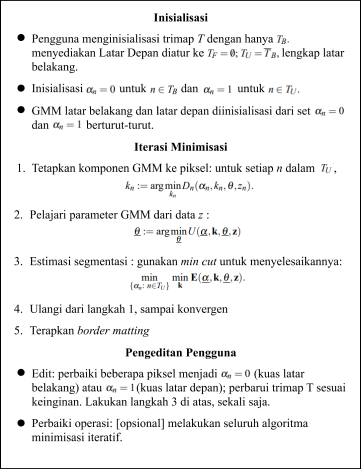
\includegraphics[width=\textwidth]{gambar/gambar-2_6.png}
    \end{subfigure}     
  \caption{
    Segmentasi gambar di \emph{GrabCut} (\cite{Rother:2004})
    }
  \label{img:segmentasi_grabcut}
\end{figure}


\begin{figure}[H]
  \centering
    \begin{subfigure}{0.3\textwidth}
      \centering{}
      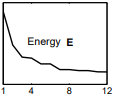
\includegraphics[width=\textwidth]{gambar/gambar-2_7(a).png}
      \caption{}
    \end{subfigure}%
    \begin{subfigure}{0.3\textwidth}
      \centering{}
      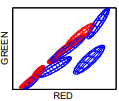
\includegraphics[width=\textwidth]{gambar/gambar-2_7(b).png}
      \caption{}
    \end{subfigure}  
    \begin{subfigure}{0.3\textwidth}
      \centering{}
      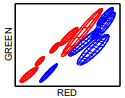
\includegraphics[width=\textwidth]{gambar/gambar-2_7(c).png}
      \caption{}
    \end{subfigure}  
  \caption{
    Konvergensi minimalisasi iteratif untuk data gambar \ref{img:2.5}(f). (a) Energi E untuk contoh 
    llama konvergen selama 12 iterasi dengan K = 5, komponen campuran digunakan untuk latar belakang (merah) dan latar depan (biru) (\cite{Rother:2004}). 
    }
    \label{img:2.7}
\end{figure}

\subsubsection{{Interaksi Pengguna dan Trimap yang Tidak Lengkap}}

\textbf{Trim tidak lengkap}. Algoritma minimisasi iteratif memungkinkan peningkatan 
keserbagunaan interaksi pengguna. Secara khusus, pelabelan yang tidak lengkap menjadi 
layak di mana, sebagai pengganti trimap T penuh, pengguna hanya perlu menentukan, 
katakanlah, wilayah latar belakang \(T_{B}\), meninggalkan \(T_{F} = 0\). Tidak ada pelabelan latar 
depan keras yang dilakukan sama sekali. Minimisasi iteratif (gambar \ref{img:2.6}) menangani 
ketidaklengkapan ini dengan mengizinkan label sementara pada beberapa piksel (di 
latar depan) yang kemudian dapat ditarik kembali; hanya label latar belakang \(T_{B}\) 
yang dianggap tegas — dijamin tidak akan ditarik kembali nantinya. (Tentu saja 
skema pelengkap, dengan label tegas untuk latar depan saja, juga memungkinkan.) 
\(T_{B}\) awal ditentukan oleh pengguna sebagai strip piksel di sekitar bagian 
luar sudut persegi yang ditandai ( ditandai dengan warna merah pada gambar \ref{img:2.5}(f))

\begin{figure}[H]
  \centering
    \begin{subfigure}{0.5\textwidth}
      \centering{}
      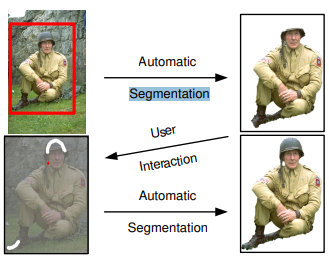
\includegraphics[width=\textwidth]{gambar/gambar-2_8.png}
    \end{subfigure}     
  \caption{
    Pengeditan pengguna. Setelah interaksi pengguna awal dan segmentasi (baris atas), 
    pengeditan pengguna lebih lanjut (gambar \ref{img:2.6}) diperlukan. (\cite{Rother:2004})
    }
    \label{img:2.8}
\end{figure}

\textbf{Pengeditan pengguna lebih lanjut.} Pelabelan pengguna awal yang tidak lengkap 
cukup sepuluh untuk memungkinkan seluruh segmentasi diselesaikan secara otomatis, 
tetapi tidak berarti selalu. Jika tidak, pengeditan pengguna lebih lanjut diperlukan, 
seperti yang ditunjukkan pada gambar \ref{img:2.8}. Ini mengambil bentuk menyikat piksel, membatasinya 
menjadi latar depan yang kokoh atau latar belakang yang kokoh; lalu minimisasi 
langkah 3. pada gambar \ref{img:2.6} diterapkan. Perhatikan bahwa cukup menyikat, secara 
kasar, hanya sebagian dari area yang salah diberi label. Selain itu, operasi "perbaiki" 
opsional dari gambar \ref{img:2.6} memperbarui model warna, mengikuti suntingan pengguna. Ini 
menopang efek operasi edit yang seringkali bermanfaat. Perhatikan bahwa untuk efisiensi 
aliran optimal, dihitung dengan \emph{graph cut}, dapat digunakan kembali selama 
pengeditan pengguna.


%!TEX root = ./template-skripsi.tex
%-------------------------------------------------------------------------------
%                            BAB III
%               			PEMBAHASAN
%-------------------------------------------------------------------------------

\chapter{METODOLOGI PENELITIAN}

\section{Desain Segmentasi Luka dengan Metode \emph{GrabCut}}
Proses pembuatan segmentasi luka, peneliti menggunakan metode 
\emph{GrabCut}. Metode segmentasi luka berupa citra gambar dengan metode \emph{GrabCut} 
berdasarkan algoritma yang telah dikembangkan oleh (\cite{Rother:2004}) adalah program 
untuk mensegmentasi citra gambar menjadi dua bagian yaitu \emph{foreground} dan
sisanya akan dianggap menjadi \emph{background}. 

Algoritma \emph{GrabCut} secara umum terdapat beberapa tahapan yaitu tahap inisiasi
kotak pembatas (\emph{bounding box}), setelah itu tahap iterasi minimisasi, dan dilanjutkan
dengan penyuntingan pengguna.

\subsection{Inisiasi Kotak Pembatas (\emph{Bounding Box})}
peneliti melakukan inisiasi \emph{bounding box} pada daerah yang melingkupi objek 
dimana daerah yang berada didalam \emph{bounding box} akan digunakan untuk membuat 
\emph{Trimap Unknown} \((T_{U})\) dan daerah di luarnya akan dianggap sebagai \emph{Trimap Background} 
atau \((T_{B})\). Setiap piksel-n yang termasuk \((T_{B})\) akan memiliki \(\alpha_{n}\) 
bernilai 0, sedangkan piksel-n dari \((T_{U})\) akan bernilai 1 untuk \(\alpha_{n}\). 
Tujuan dari \emph{bounding box} ialah untuk mempercepat waktu komputasi dari 
algoritma serta meningkatkan tingkat akurasi segmentasi.

\begin{figure}[H]
	\centering
	  \begin{subfigure}{0.3\textwidth}
		\centering{}
		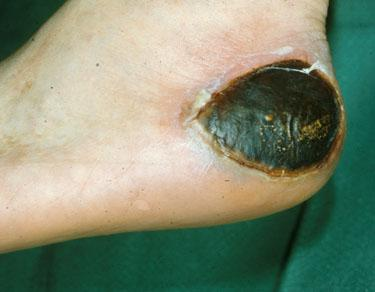
\includegraphics[width=\textwidth]{gambar/gambar-3_2(b).jpg}
		\caption{}
	  \end{subfigure}  
	  \begin{subfigure}{0.3\textwidth}
		\centering{}
		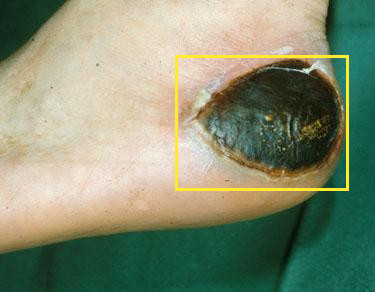
\includegraphics[width=\textwidth]{gambar/rectangle.png}
		\caption{}
	  \end{subfigure}
	\caption{
		(a) Data citra luka 2.png, (b) Inisasi kotak pembatas
        }
  \end{figure}

\subsection{Implementasi Algoritma \emph{GrabCut}}
Setelah kotak tergambar, pada tahap ini terdapat beberapa algoritma yaitu inisiasi 
dan mempelajari \emph{Gaussian Mixture Models} (GMM), dan segmentasi citra \emph{GraphCut}. 
Inisiasi GMM digunakan untuk memperoleh nilai probabilistik dari tiap piksel yang ada
didalam \((T_{U})\). GMM terdiri dari beberapa parameter yaitu \textbf{K} komponen, 
rata-rata \(\mu\), matriks kovarians \(\Sigma\), dan probabilitas prior \(\omega\). 
Selanjutnya mempelajari parameter GMM yang berdasarkan probabilitas dari parameter 
GMM tiap piksel.

Setelah mempelajari parameter GMM dari tiap piksel, maka diperoleh nilai parameter
untuk komponen yang ada pada setiap piksel, masuk ke tahap segmentasi citra luka 
dengan menggunakan algoritma \emph{GraphCut}. Algoritma ini memvisualisasikan tiap piksel 
dari citra sebagai sebuah graf yang saling terhubung, satuan piksel pada gambar bisa
disebut sebagai \emph{node} pada graf yang mana tiap node akan memiliki komponen yang 
berasal dari nilai GMM tadi, pada graf yang sudah terbentuk maka akan ada dua terminal
yaitu terminal \emph{source} dan terminal \emph{sink}, partisi graf (kumpulan \emph{node}) 
yang memiliki hubungan probabilitas ke terminal \emph{source} akan menjadi \emph{foreground}
dan partisi graf yang memiliki hubungan probabilitas ke terminal \emph{sink} akan
menjadi \emph{background}. Algoritma ini memanfaatkan nilai dari GMM yang sudah dipelajari dan \emph{term smoothness}, nilai GMM akan dipakai sebagai
kemungkinan piksel yang termasuk \emph{background} atau \emph{foreground} sedangkan 
\emph{term smoothness} dipakai untuk menghitung hubungan diskontinuitas antar piksel.

\begin{figure}[H]
	\centering{}
	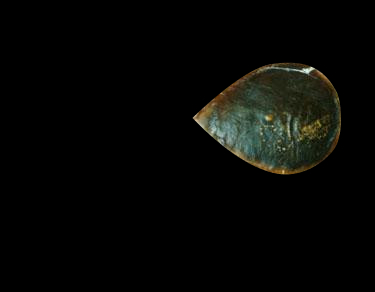
\includegraphics[width=0.4\textwidth]{gambar/res_2.png}
	\caption{Hasil segmentasi dengan \emph{GrabCut}}
  \end{figure}

% \subsection{Penyuntingan oleh Pengguna}
% Langkah selanjutnya melakukan perbaikan dari citra yang sudah di segmentasi
% dari hasil sebelumnya dengan menetapkan piksel yang seharusnya menjadi latar belakang
% atau latar depan dengan melakukan langkah \emph{mincut} yang dilakukan sekali.

% \begin{figure}[H]
% 	\centering
%       \begin{subfigure}{0.3\textwidth}
% 		\centering{}
% 		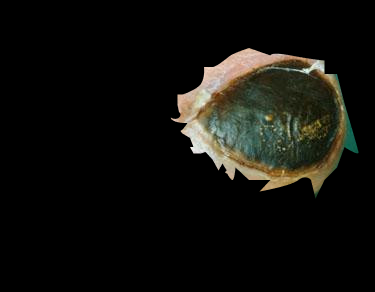
\includegraphics[width=\textwidth]{gambar/res_1.png}
% 		\caption{}
% 	  \end{subfigure}
%       \begin{subfigure}{0.3\textwidth}
% 		\centering{}
% 		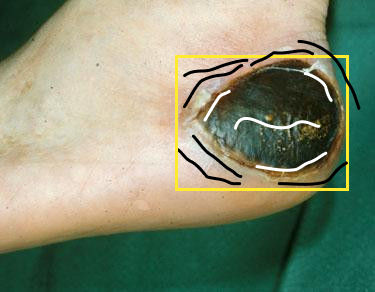
\includegraphics[width=\textwidth]{gambar/brush.png}
% 		\caption{}
% 	  \end{subfigure}
%       \begin{subfigure}{0.3\textwidth}
% 		\centering{}
% 		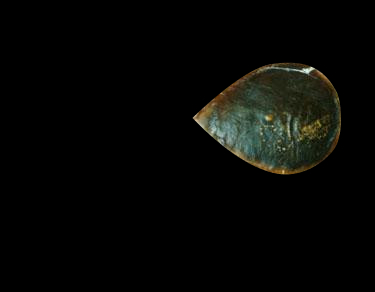
\includegraphics[width=\textwidth]{gambar/res_2.png}
% 		\caption{}
% 	  \end{subfigure}
% 	\caption{
% 		(a) Hasil \emph{Grabcut} sebelum diperbaiki, (b) Penyuntingan oleh pengguna, (c) Hasil 
%         segmentasi \emph{GrabCut} setelah diperbaiki
% 	 }
%   \end{figure}

\section{Diagram Alir Segmentasi Luka dengan Metode \emph{GrabCut}}
Berikut adalah diagram alir segmentasi luka dengan metode \emph{GrabCut}: 
\begin{figure}[H]
	\centering{}
	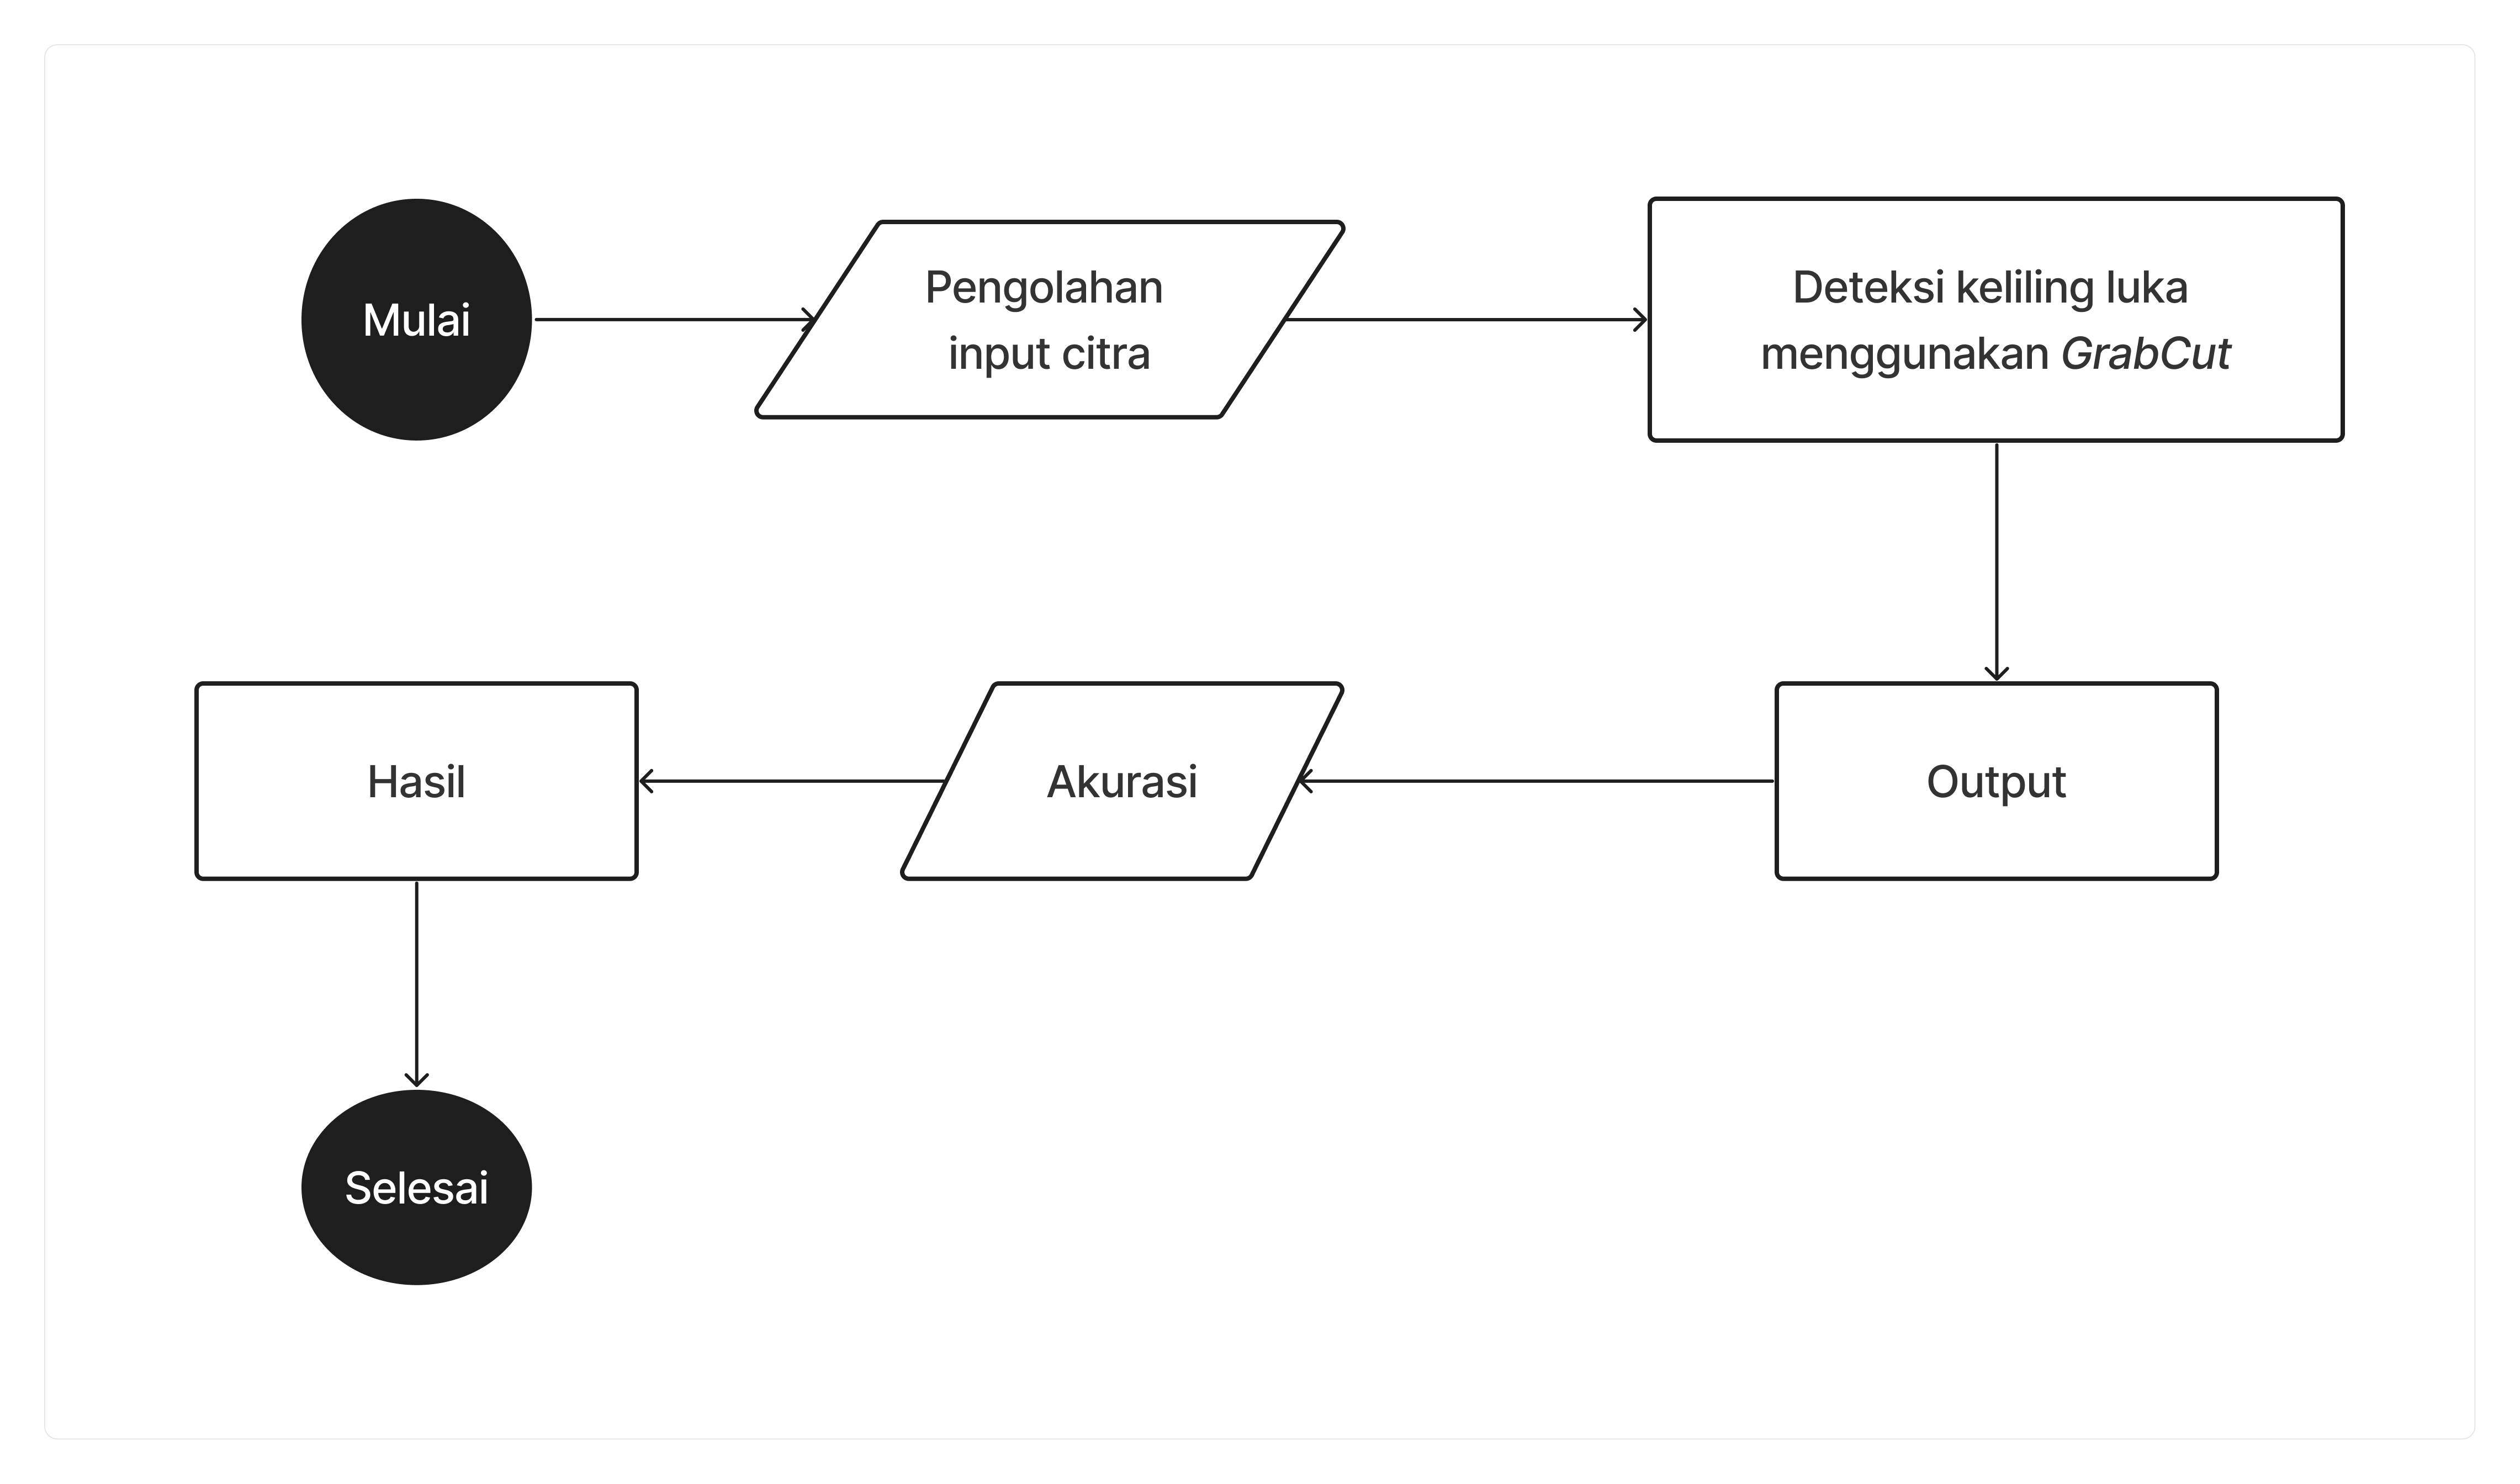
\includegraphics[width=0.8\textwidth]{gambar/diagram_penelitian.png}
	\caption{Diagram alir penelitian}
	\label{img:diagram_penelitian}
  \end{figure}

\begin{figure}[H]
	\centering{}
	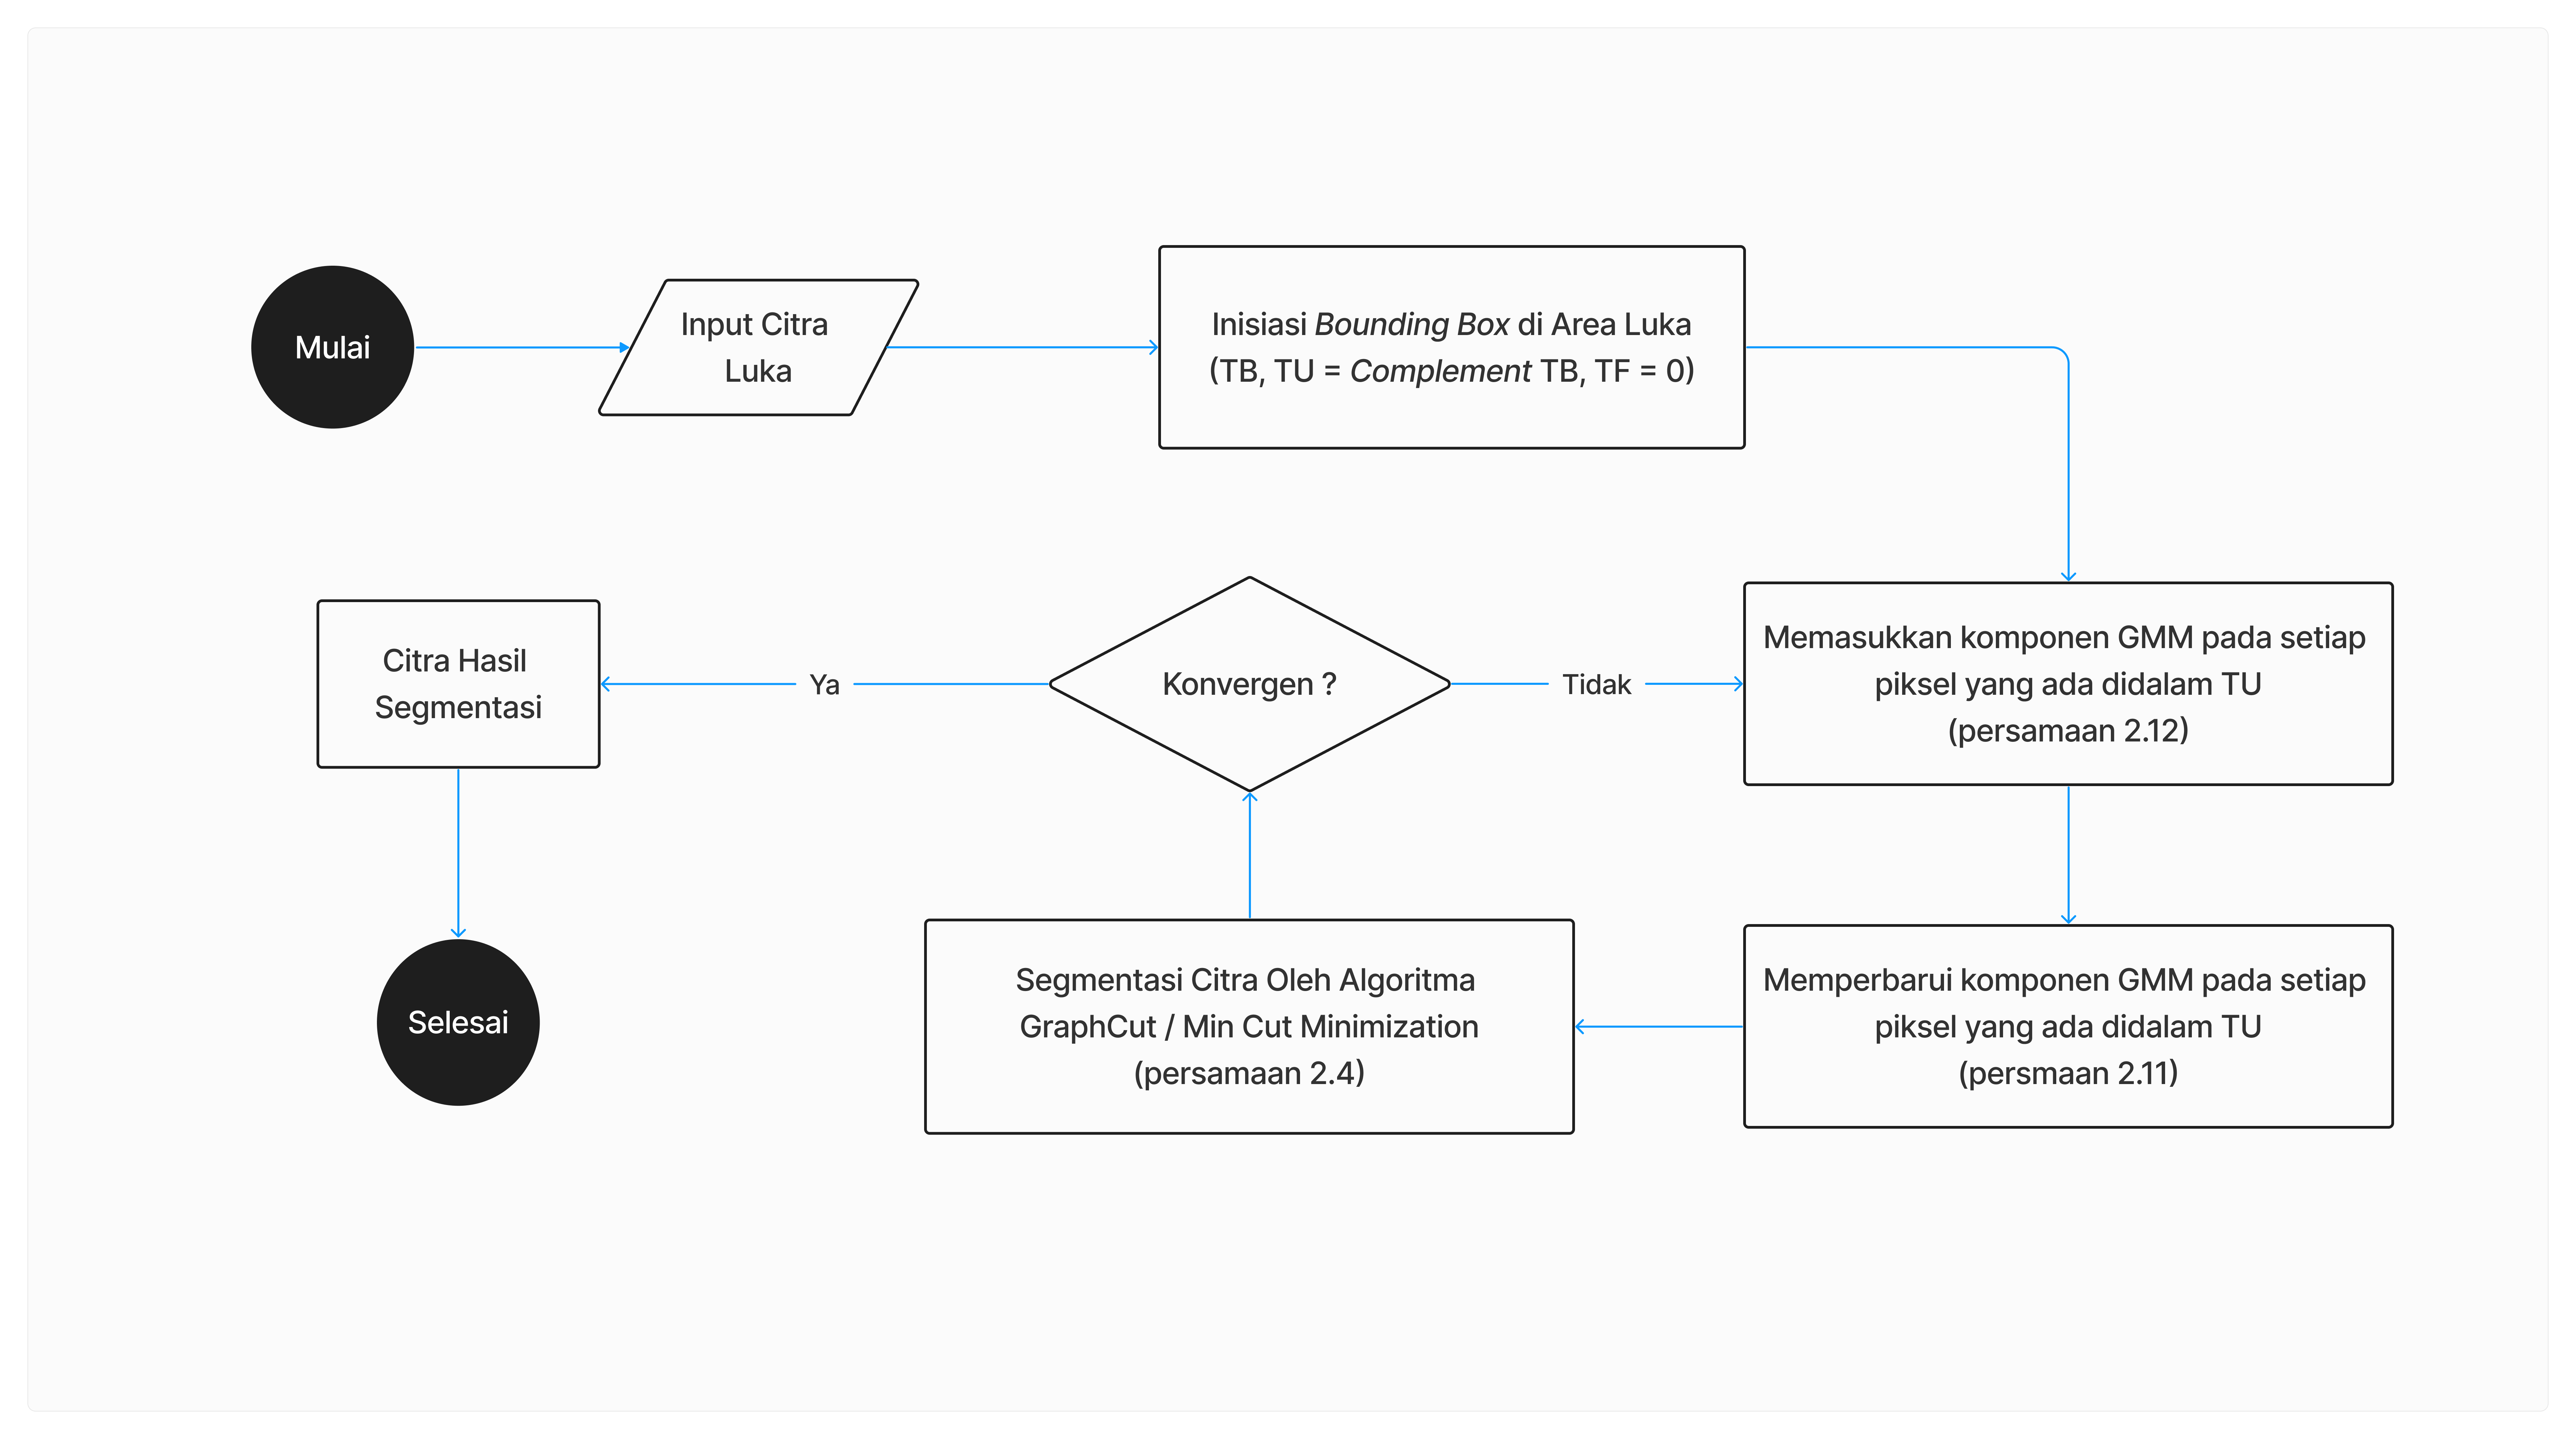
\includegraphics[width=0.9\textwidth]{gambar/diagram_grabcut.png}
	\caption{Diagram alir metode \emph{GrabCut}}
  \end{figure}

\begin{figure}[H]
	\centering{}
	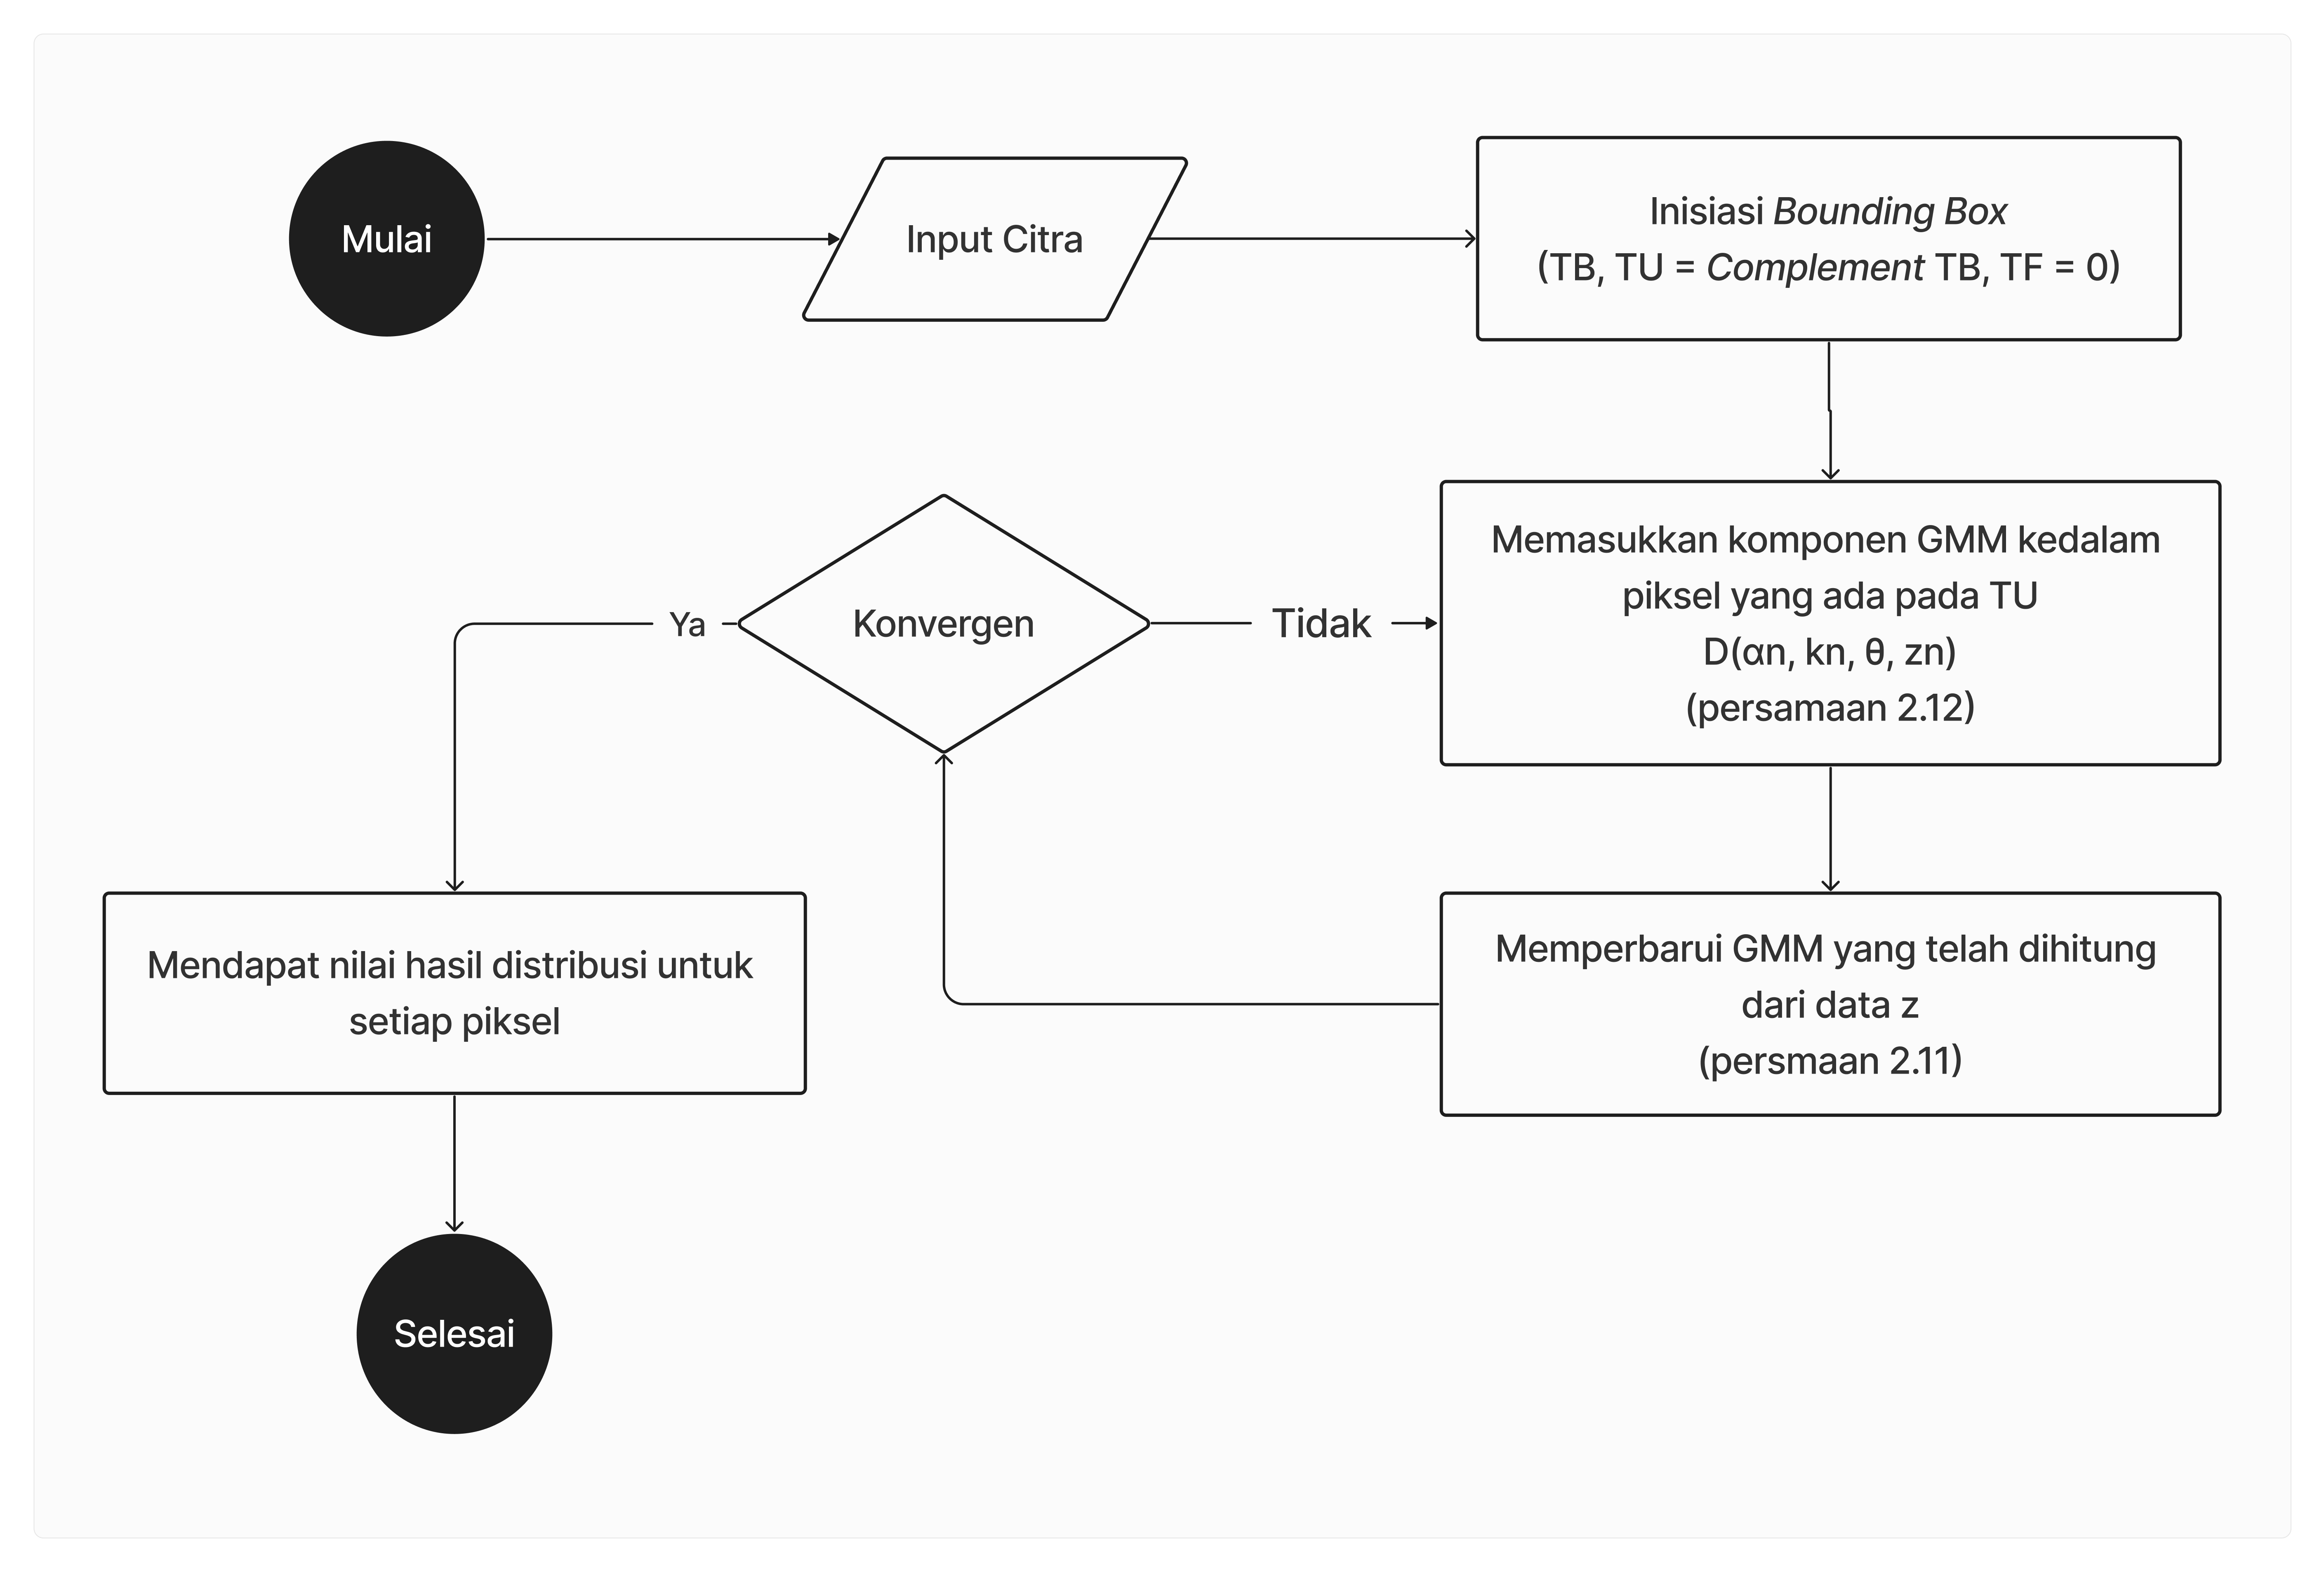
\includegraphics[width=0.9\textwidth]{gambar/diagram_gmm.png}
	\caption{Diagram alir tahap \emph{Gaussian Mixture Models}}
  \end{figure}

\section{Struktur Data}

\subsection{\emph{Node}}

\emph{Node} merupakan elemen dasar dalam pembentukan struktur data seperti \emph{linked list},
pohon, dan graf. Sebuah \emph{node} setidaknya terdiri dari dua komponen, yaitu 
data atau nilai dari \emph{node} tersebut dan referensi atau tautan yang menghubungkan 
\emph{node} tersebut dengan \emph{node} lainnya. Peneliti menggunakan struktur data \emph{node} untuk merepresentasikan piksel dari
citra luka, setiap piksel dari gambar menyimpan beberapa informasi, di antaranya komponen warna
RGB (\emph{Red,Green,Blue}), komponen GMM dan nilai label piksel.

\begin{figure}[H]
	\centering{}
	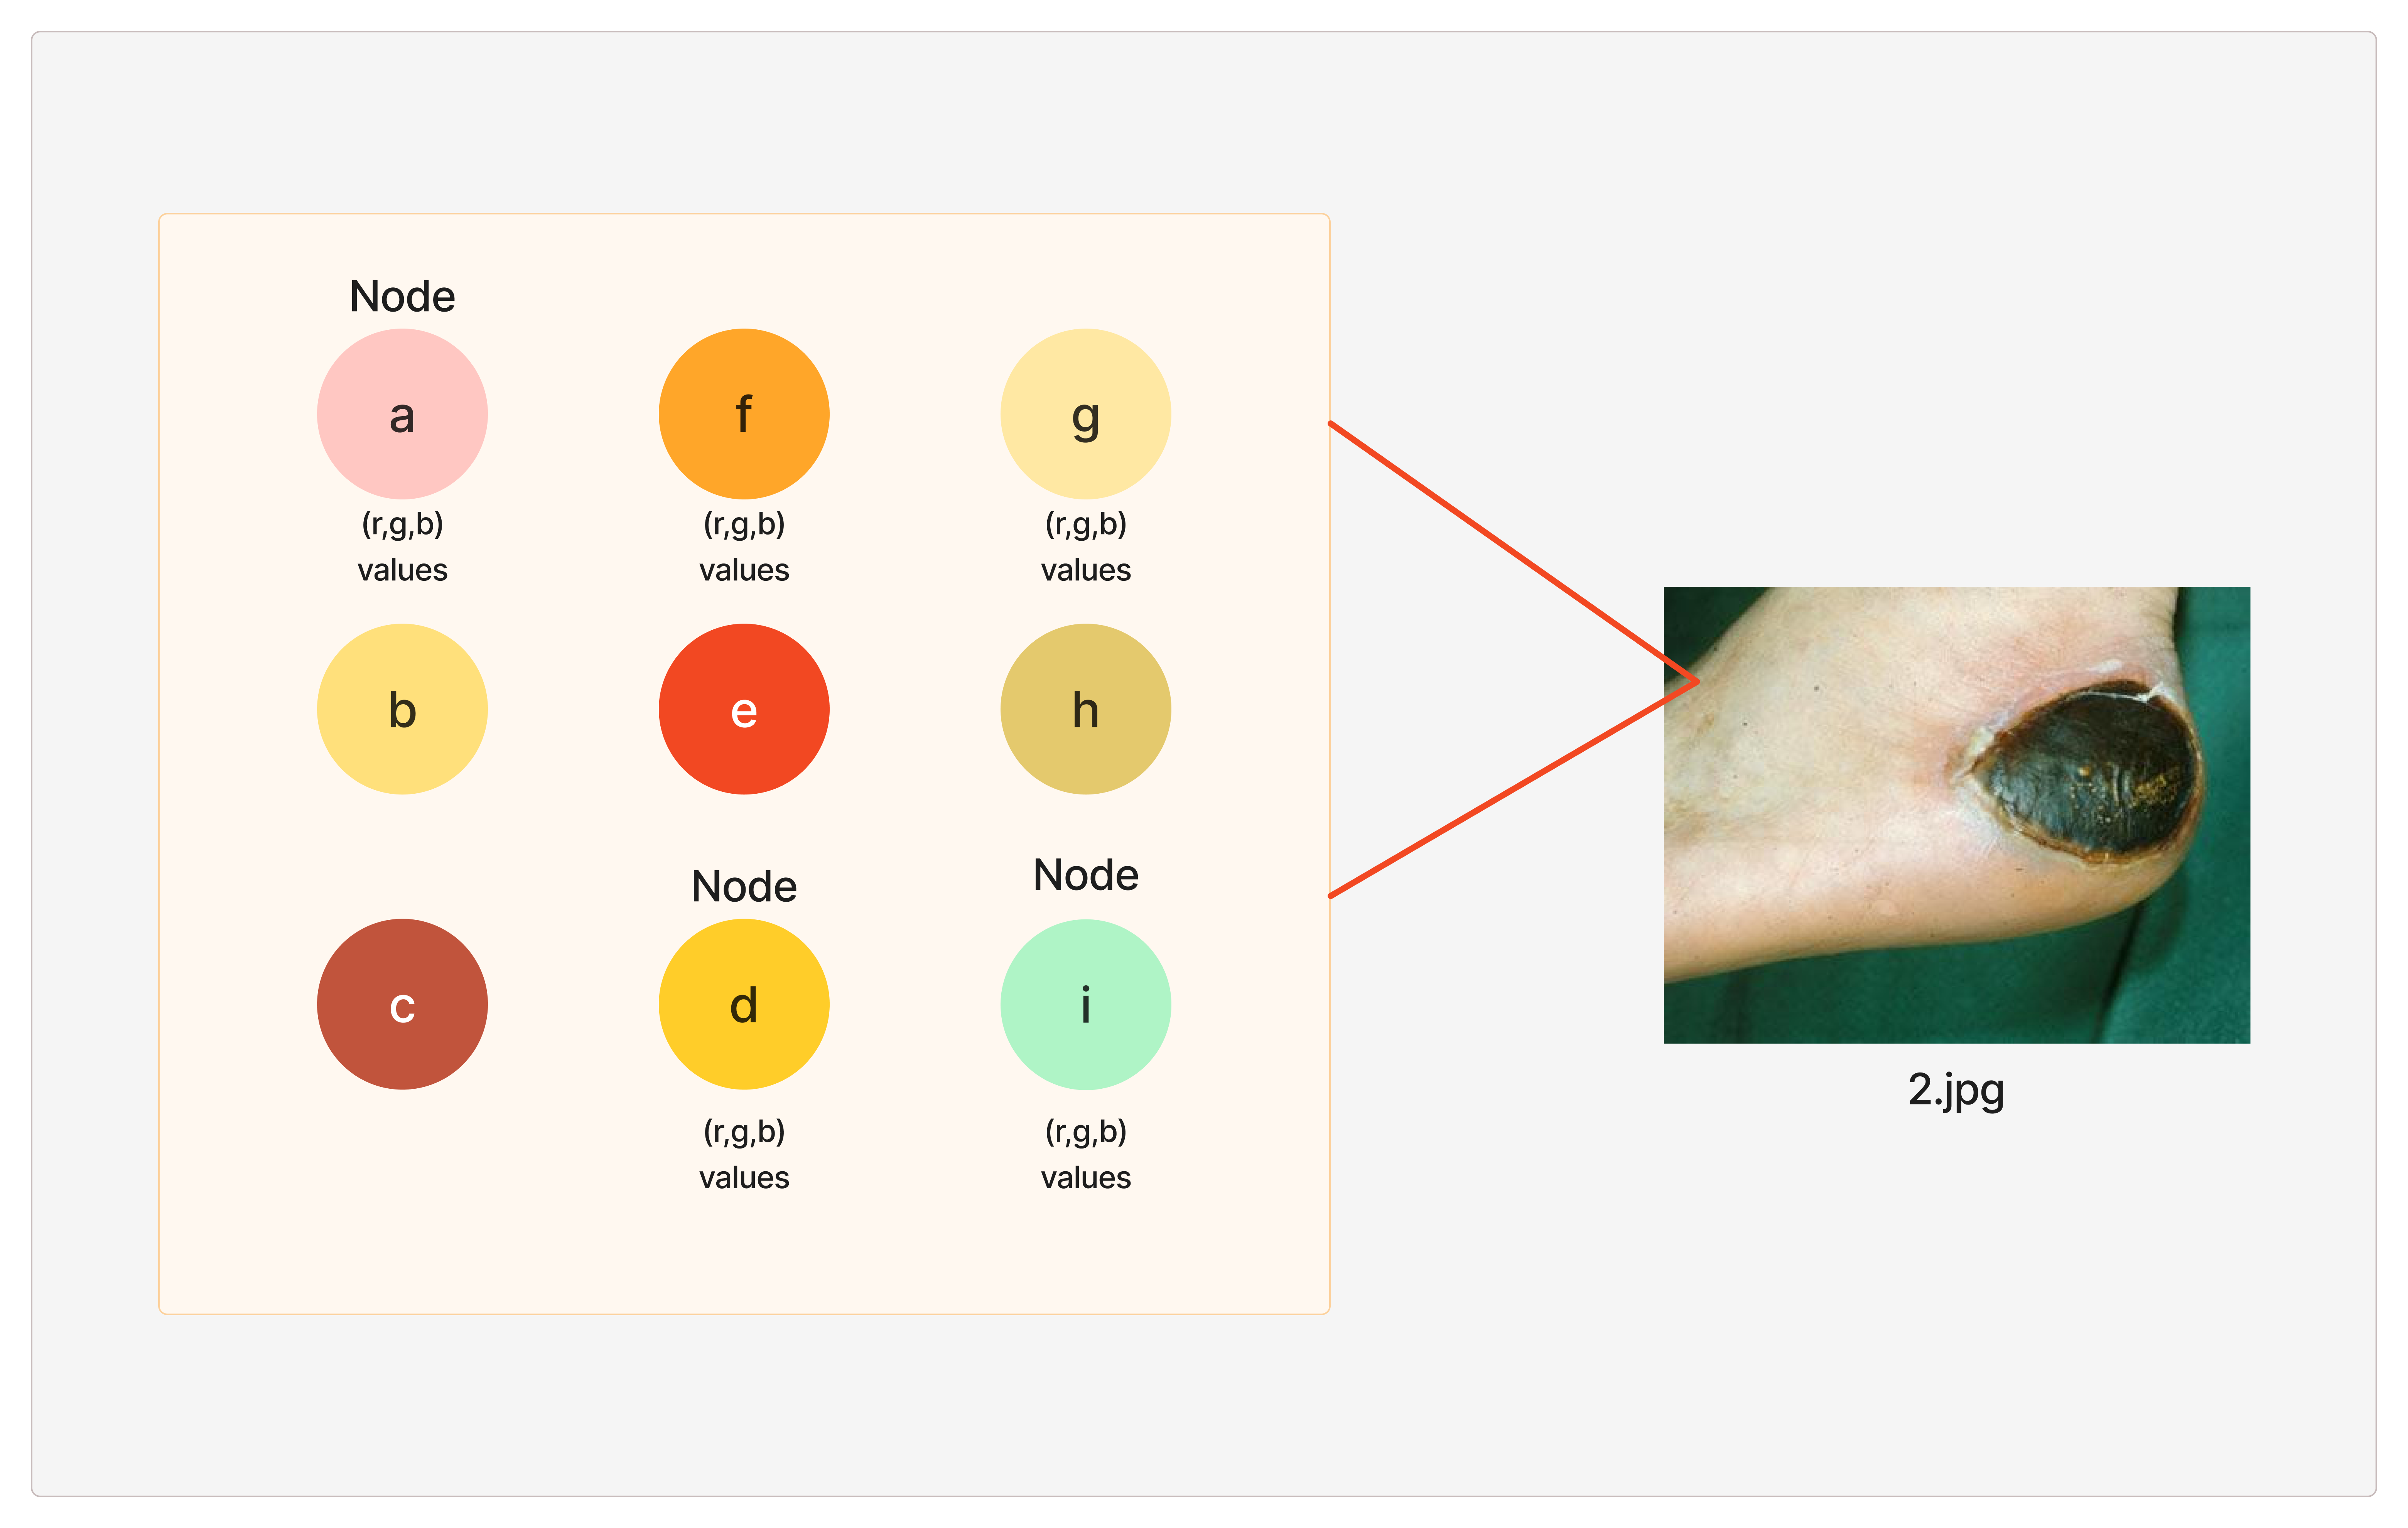
\includegraphics[width=0.5\textwidth]{gambar/node_representasi.png}
	\caption{Representasi \emph{node} terhadap piksel pada gambar}
\end{figure}

Tiap informasi yang ada pada \emph{node} akan dipergunakan dalam algoritma \emph{mincut}
dengan struktur data sebagai berikut :

\begin{lstlisting} [language=C++, caption=Struktur data \emph{node}]
// Struktur Data Node dari piksel
class Node {
    public:
        bool isForeground;
        double foregroundProbability;
        double backgroundProbability;
        vector<GaussianComponent> gmmComponents;
}  
\end{lstlisting}

\subsection{\emph{Linkedlist}} 
Secara umum komponen yang ada \emph{node} diantaranya data yang disimpan dan 
referensi kepada \emph{node} selanjutnya, \emph{linkedlist} akan terbentuk 
dari rangkaian \emph{node} yang saling terhubung.

\begin{figure}[H]
	\centering{}
	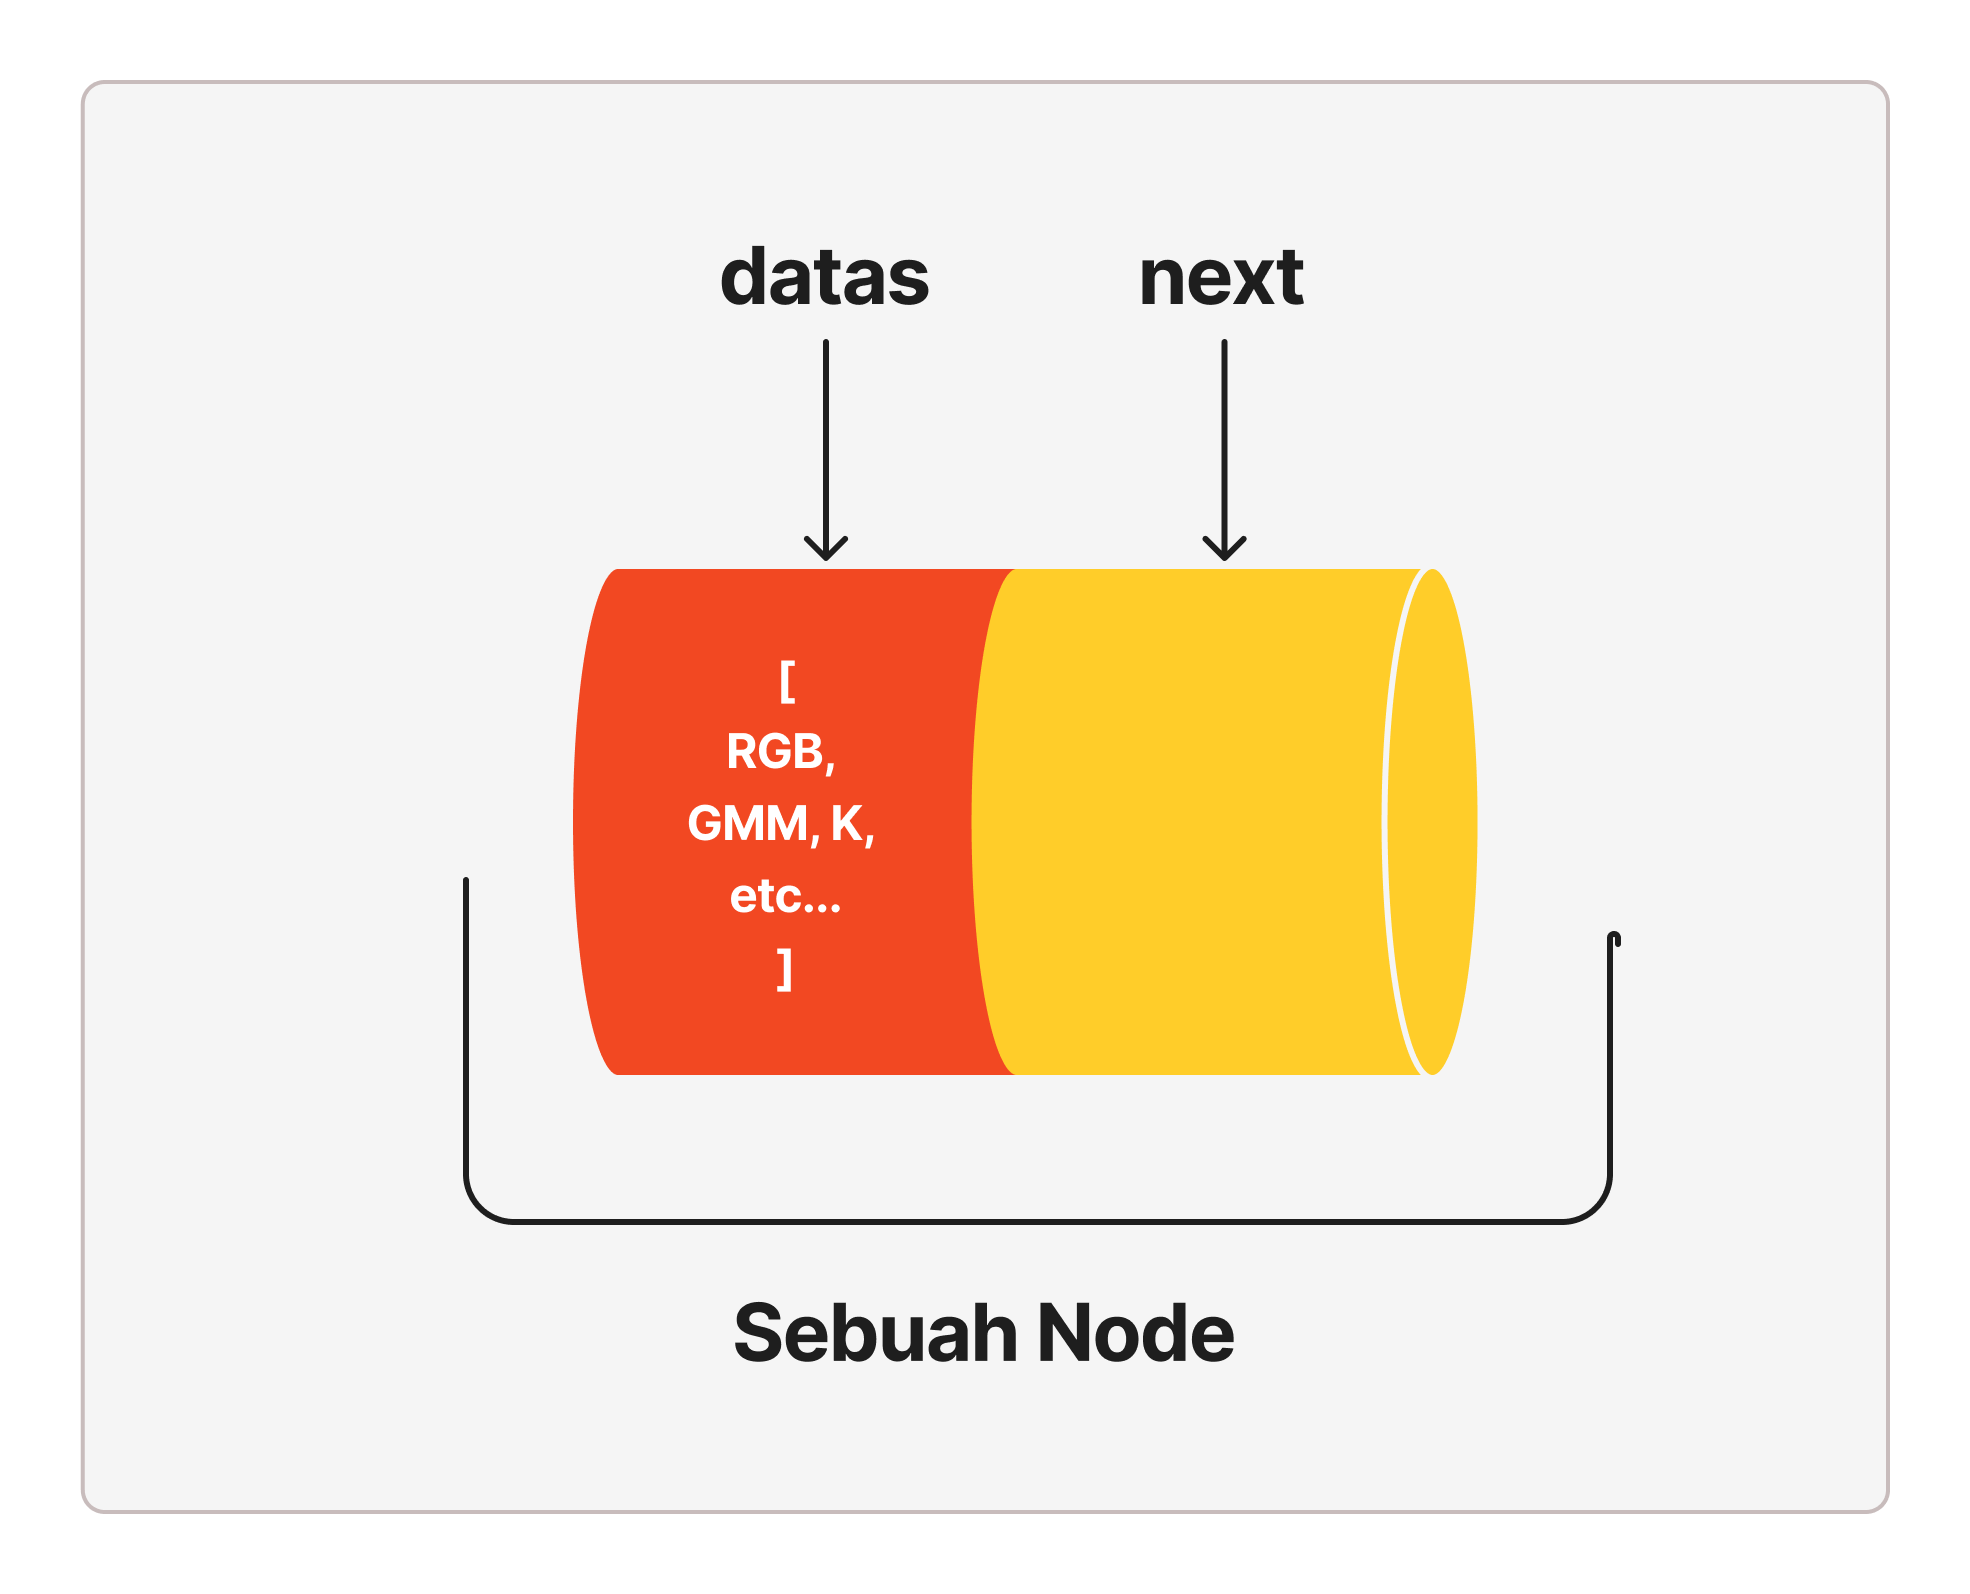
\includegraphics[width=0.6\textwidth]{gambar/node_komponen.png}
	\caption{Komponen yang ada pada sebuah \emph{node}}
\end{figure}

Pada penelitian ini struktur komponen \emph{node} yang akan peneliti gunakan 
memiliki tiga komponen yaitu referensi ke \emph{node} sebelumnya, data dari \emph{node},
dan referensi ke \emph{node} selanjutnya.

\begin{figure}[H]
	\centering{}
	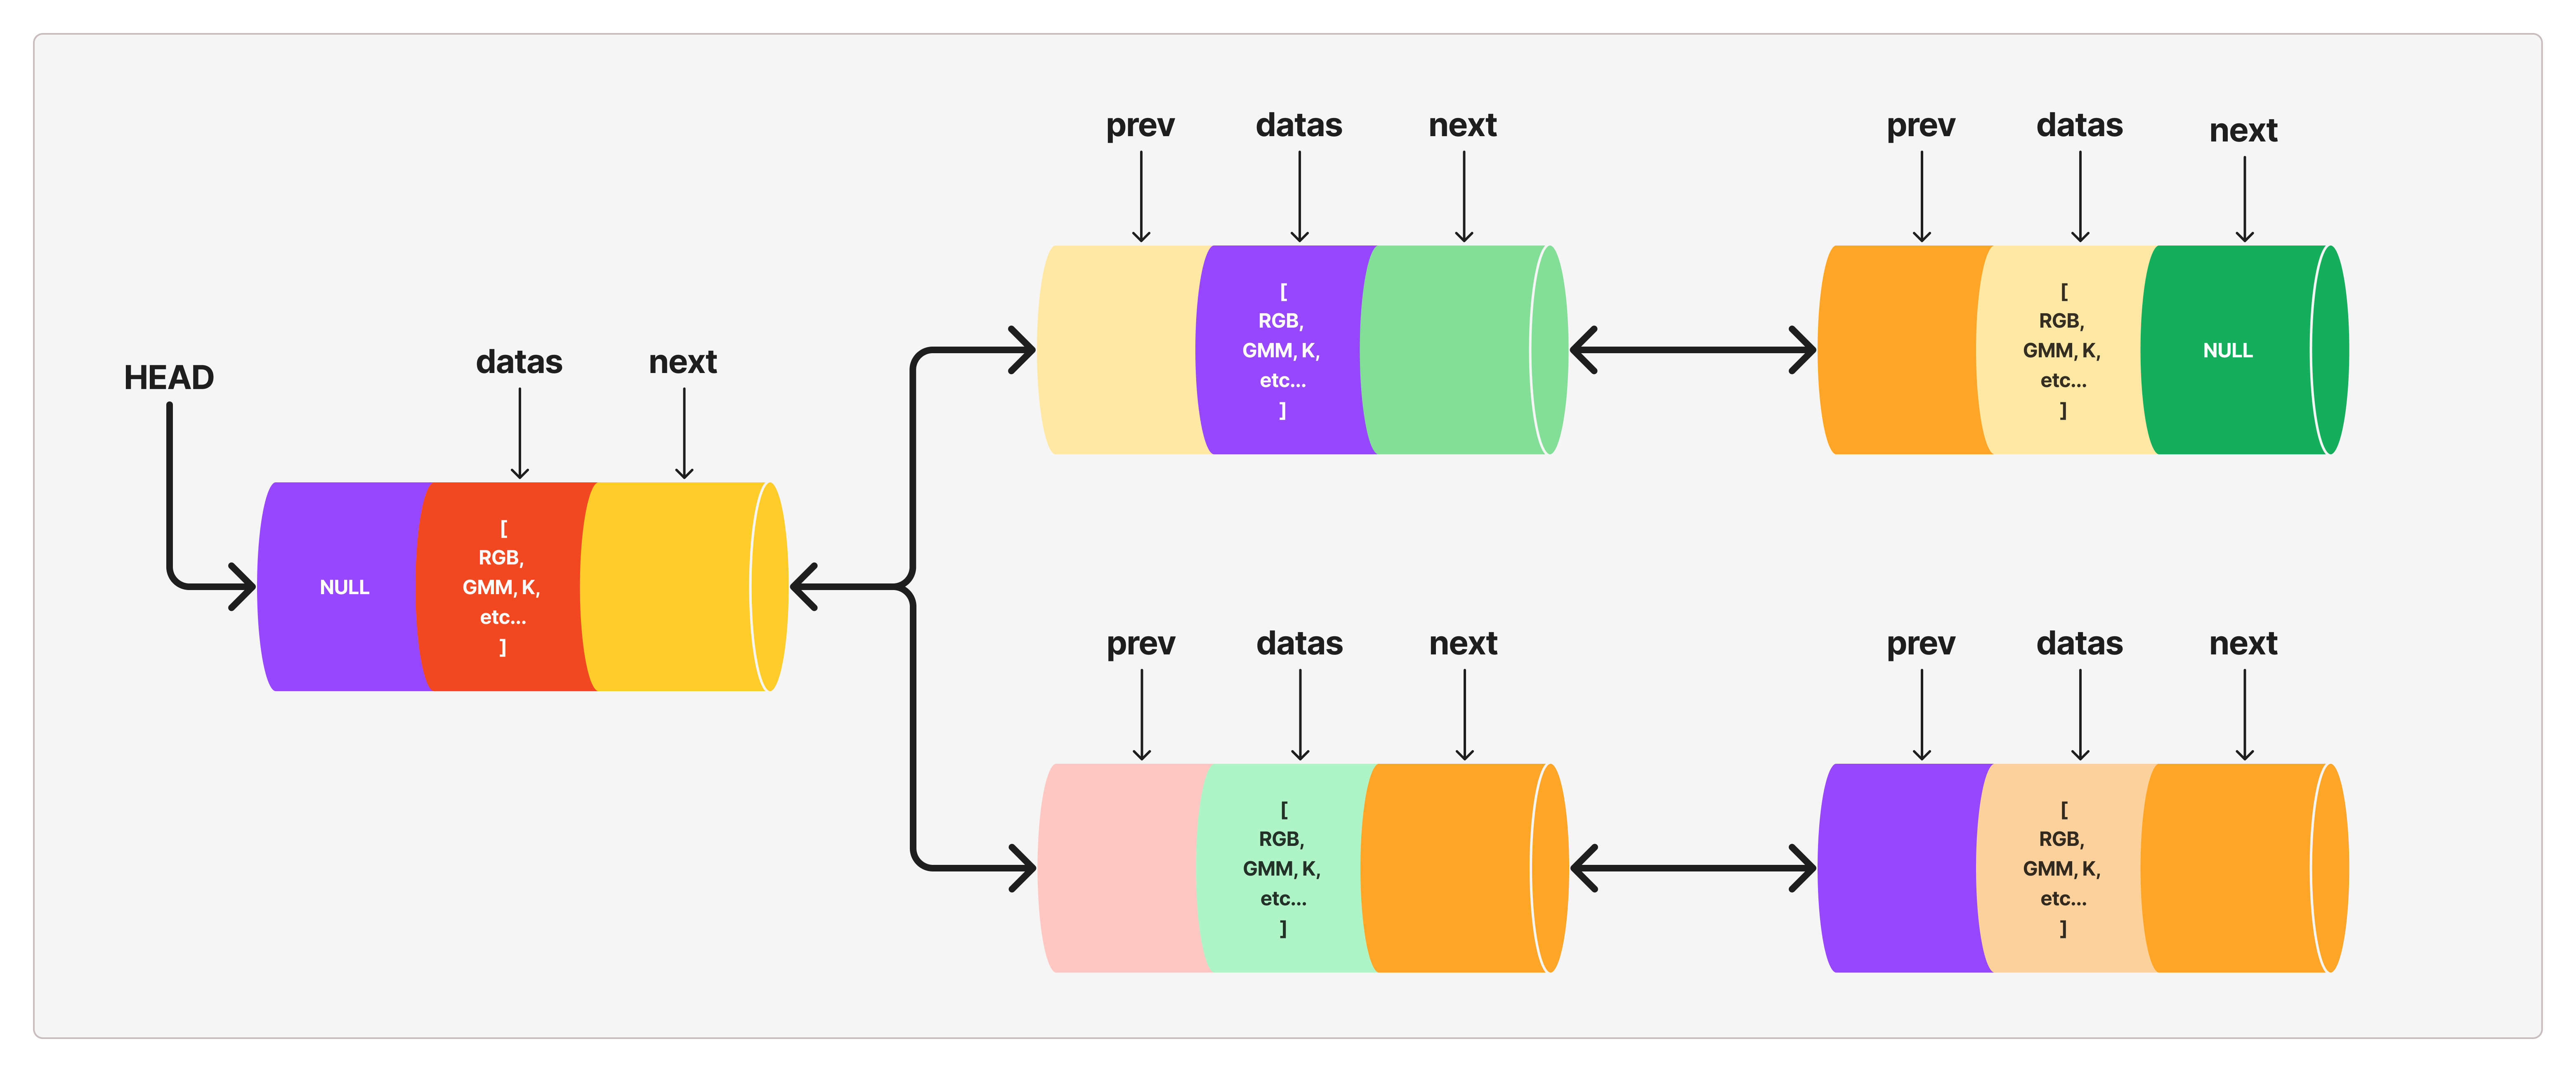
\includegraphics[width=\textwidth]{gambar/linkedlist_example.png}
	\caption{\emph{Linkedlist} terdiri dari susunan \emph{node}}
\end{figure}

Referensi pada \emph{node} bertujuan untuk mengetahui \emph{node} mana yang 
menjadi \emph{parent} menggunakan referensi ke \emph{node} sebelumnya  dan 
\emph{child} menggunakan referensi ke \emph{node} selanjutnya. \emph{Node} yang berada di awal graf akan menjadi \emph{head} dan \emph{node}
terakhir akan ditetapkan sebagai \emph{tail}, sementara komponen data-data
\emph{node} akan disimpan sebagai karakteristik dari \emph{node} tersebut.

\begin{lstlisting} [language=C++, caption=Struktur data \emph{doubly linkedlist}]
// Struktur Data LinkedList
class Node {
public:
    bool isForeground;
    double foregroundProbability;
    double backgroundProbability;
    vector<GaussianComponent> gmmComponents;

    Node* parent;
    vector<Node*> children;

    Node(bool isForeground, 
            double foregroundProbability, 
            double backgroundProbability ) {

        this->isForeground = isForeground;
        this->foregroundProbability = 
        foregroundProbability;
        this->backgroundProbability = 
        backgroundProbability;
        
        this->parent = nullptr;
    }
 	}
\end{lstlisting}


\subsection{\emph{Tree}}
Struktur data \emph{tree} merupakan suatu struktur data hirarki, \emph{tree} diibaratkan
sebagai hubungan induk dan anak dalam sebuah pohon, \emph{node} paling atas dari 
\emph{tree} disebut dengan akar (\emph{root}), dan \emph{node} turunannya disebut 
sebagai anak dari \emph{node} lain atau menjadi daun (\emph{node} yang tidak memiliki 
anak)
\begin{figure}[H]
	\centering{}
	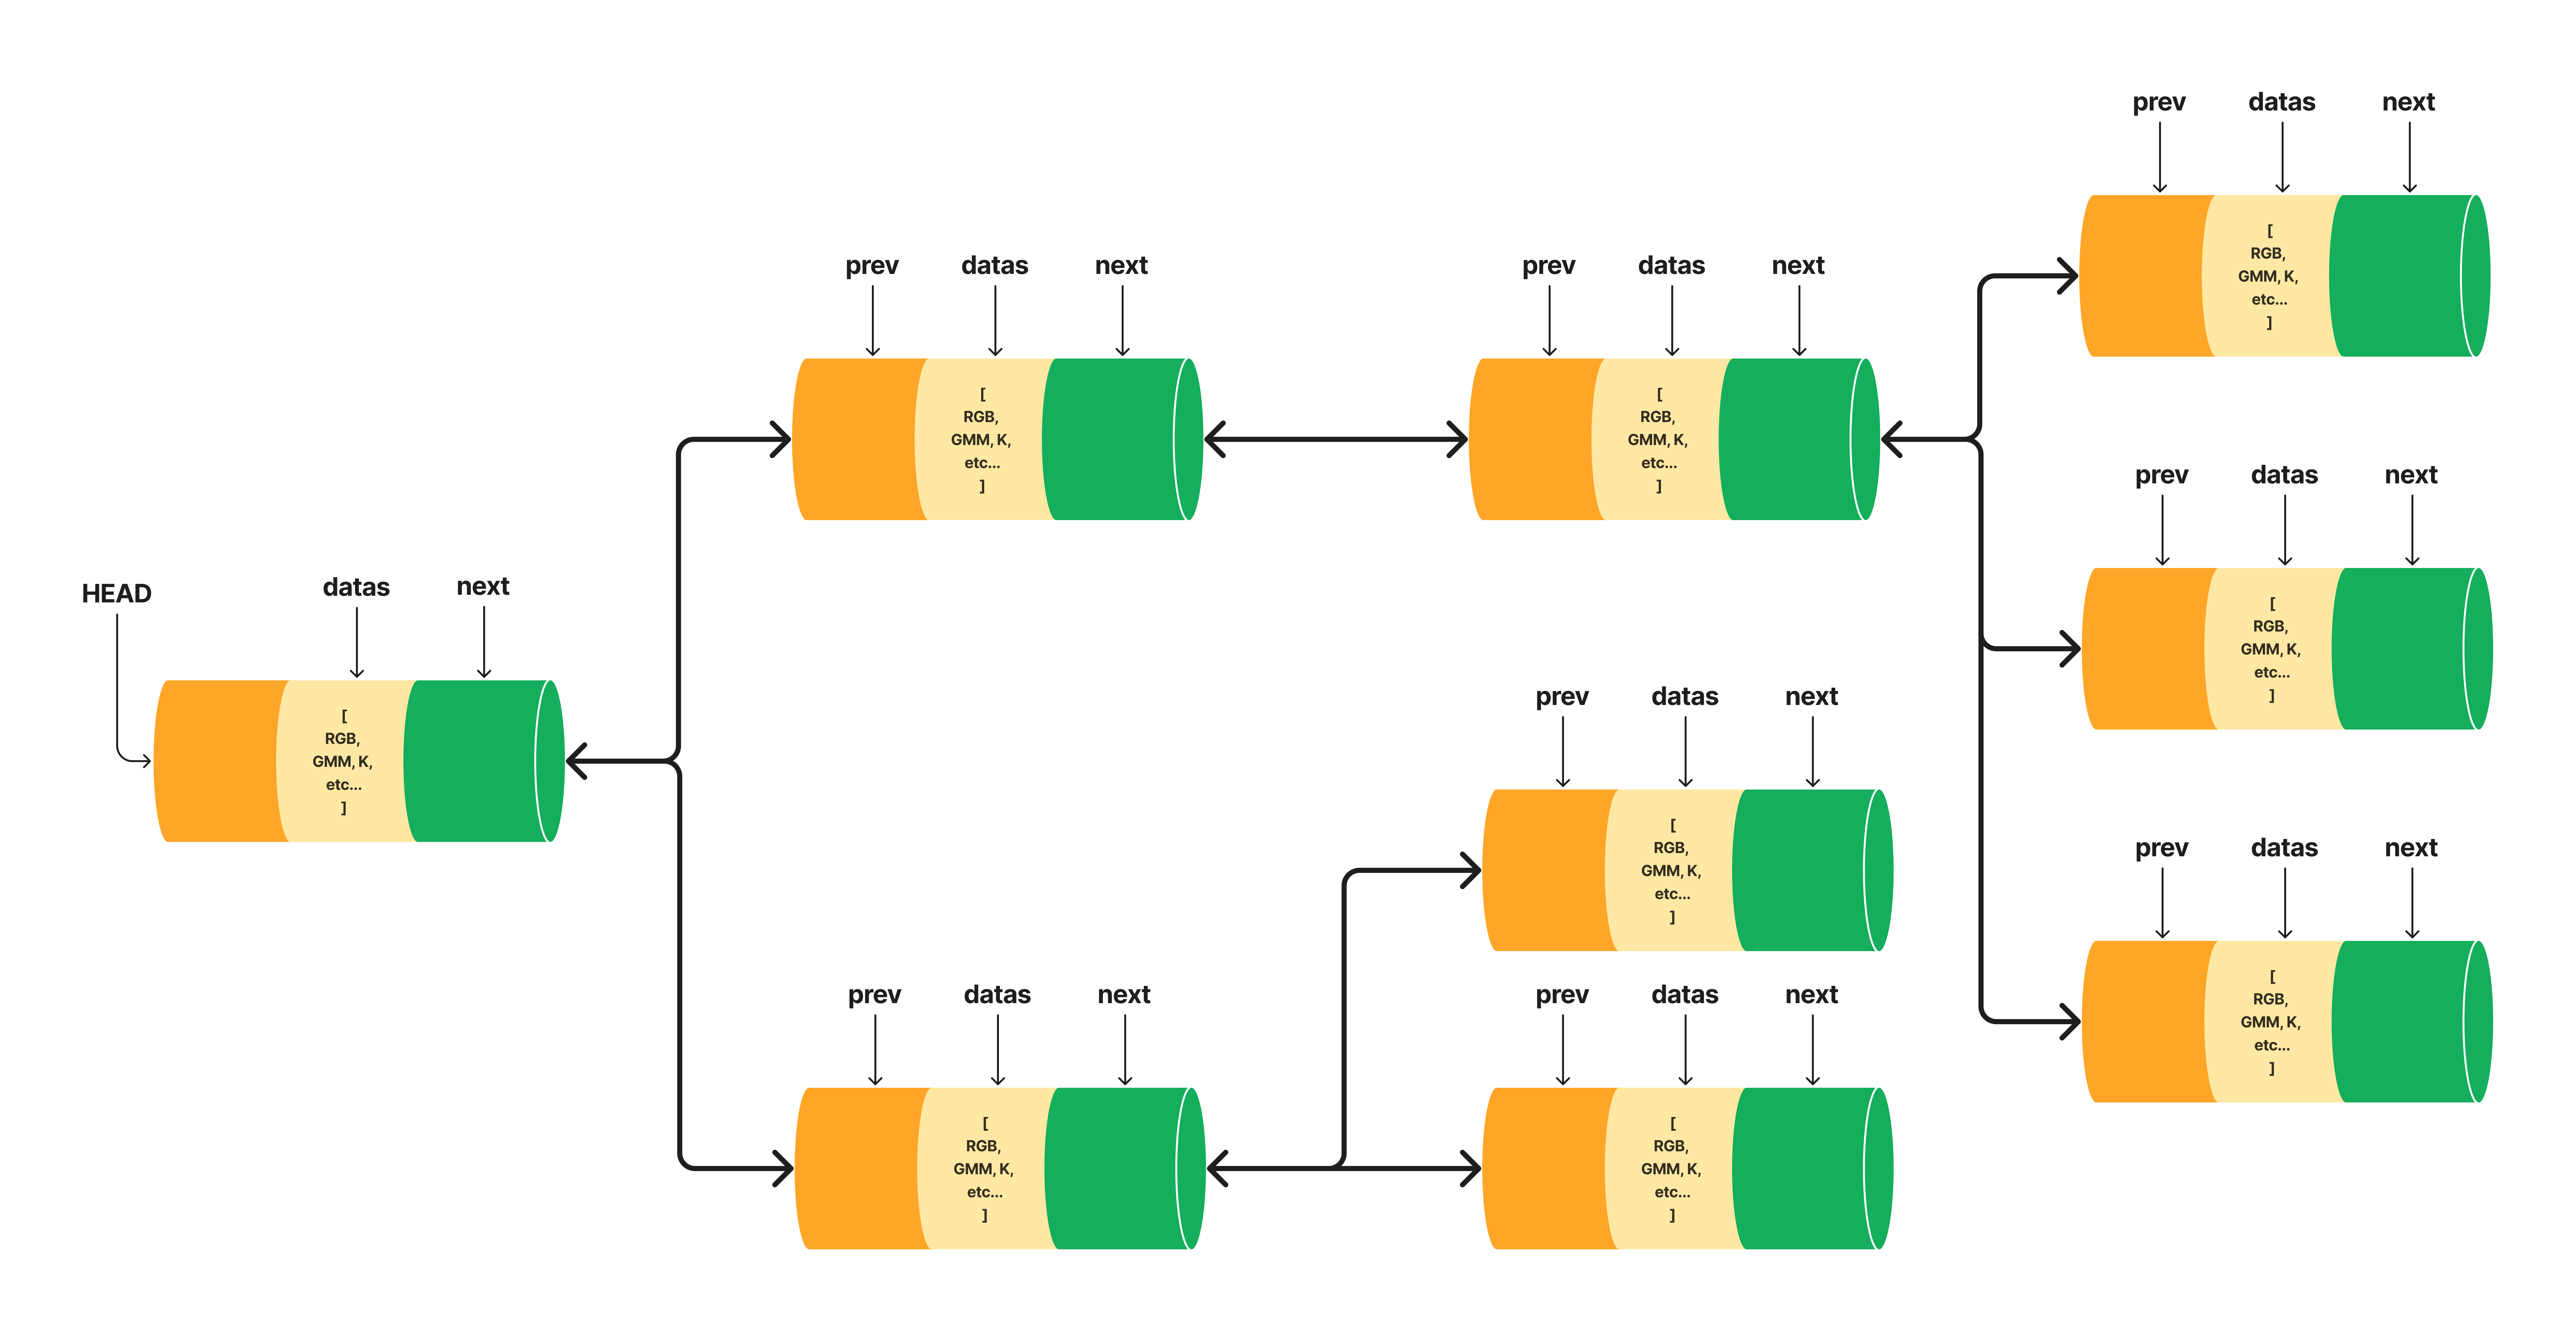
\includegraphics[width=0.8\textwidth]{gambar/tree_example.png}
	\caption{Representasi struktur data \emph{tree}}
\end{figure}

sehingga struktur data yang terbentuk dari \emph{tree} adalah sebagai berikut: 

\begin{lstlisting} [language=C++, caption=Struktur data \emph{tree}]
class Node {
    public:
        bool isForeground;
        double foregroundProbability;
        double backgroundProbability;
        vector<GaussianComponent> gmmComponents;

        Node* parent;
        vector<Node*> children;

        Node(bool isForeground, 
                double foregroundProbability, 
                double backgroundProbability ) {

            this->isForeground = isForeground;

            this->foregroundProbability = 
			foregroundProbability;

            this->backgroundProbability = 
			backgroundProbability;

            this->parent = nullptr;
        }
}

class Tree {
    private:
        Node* root;
    public:
        Tree() {
            root = nullptr;
        }

        Node* createNode(
            bool isForeground, 
            double foregroundProbability, 
            double backgroundProbability) {

            Node* newNode = new Node(
                isForeground, 
                foregroundProbability, 
                backgroundProbability);
            return newNode;
        }

        void insertChild(Node* parent, Node* child) {
            if (parent == nullptr || child == nullptr)
                return;

            child->parent = parent;
            parent->children.push_back(child);
        }
};

\end{lstlisting}

% ''' kalau mau dilanjutkan hingga di print '''
% int main() {
%     Tree tree;

%     Node* root = tree.createNode(0);
%     Node* child1 = tree.createNode(1);
%     Node* child2 = tree.createNode(2);
%     Node* child3 = tree.createNode(3);
%     Node* child4 = tree.createNode(4);
%     Node* child5 = tree.createNode(5);
%     Node* child6 = tree.createNode(6);
%     Node* child7 = tree.createNode(7);  
%     Node* child8 = tree.createNode(8);  


%     tree.insertChild(root, child1);
%     tree.insertChild(root, child2);
%     tree.insertChild(child1, child3);
%     tree.insertChild(child2, child4);
%     tree.insertChild(child2, child5);
%     tree.insertChild(child3, child6);
%     tree.insertChild(child3, child7);
%     tree.insertChild(child3, child8);

%     return 0;
% }

\subsection{Graf}
Struktur data graf dipakai untuk merepresentasikan gambar citra luka, citra yang
diinput akan berbentuk matriks dua dimensi yang mana terdiri dari baris, kolom, 
dan ranah warna RGB, graf selanjutnya dibangun dan menghubungkan antar \emph{node}
piksel, peneliti membuat ilustrasi dari graf sebagai berikut 

\begin{figure}[H]
	\centering{}
	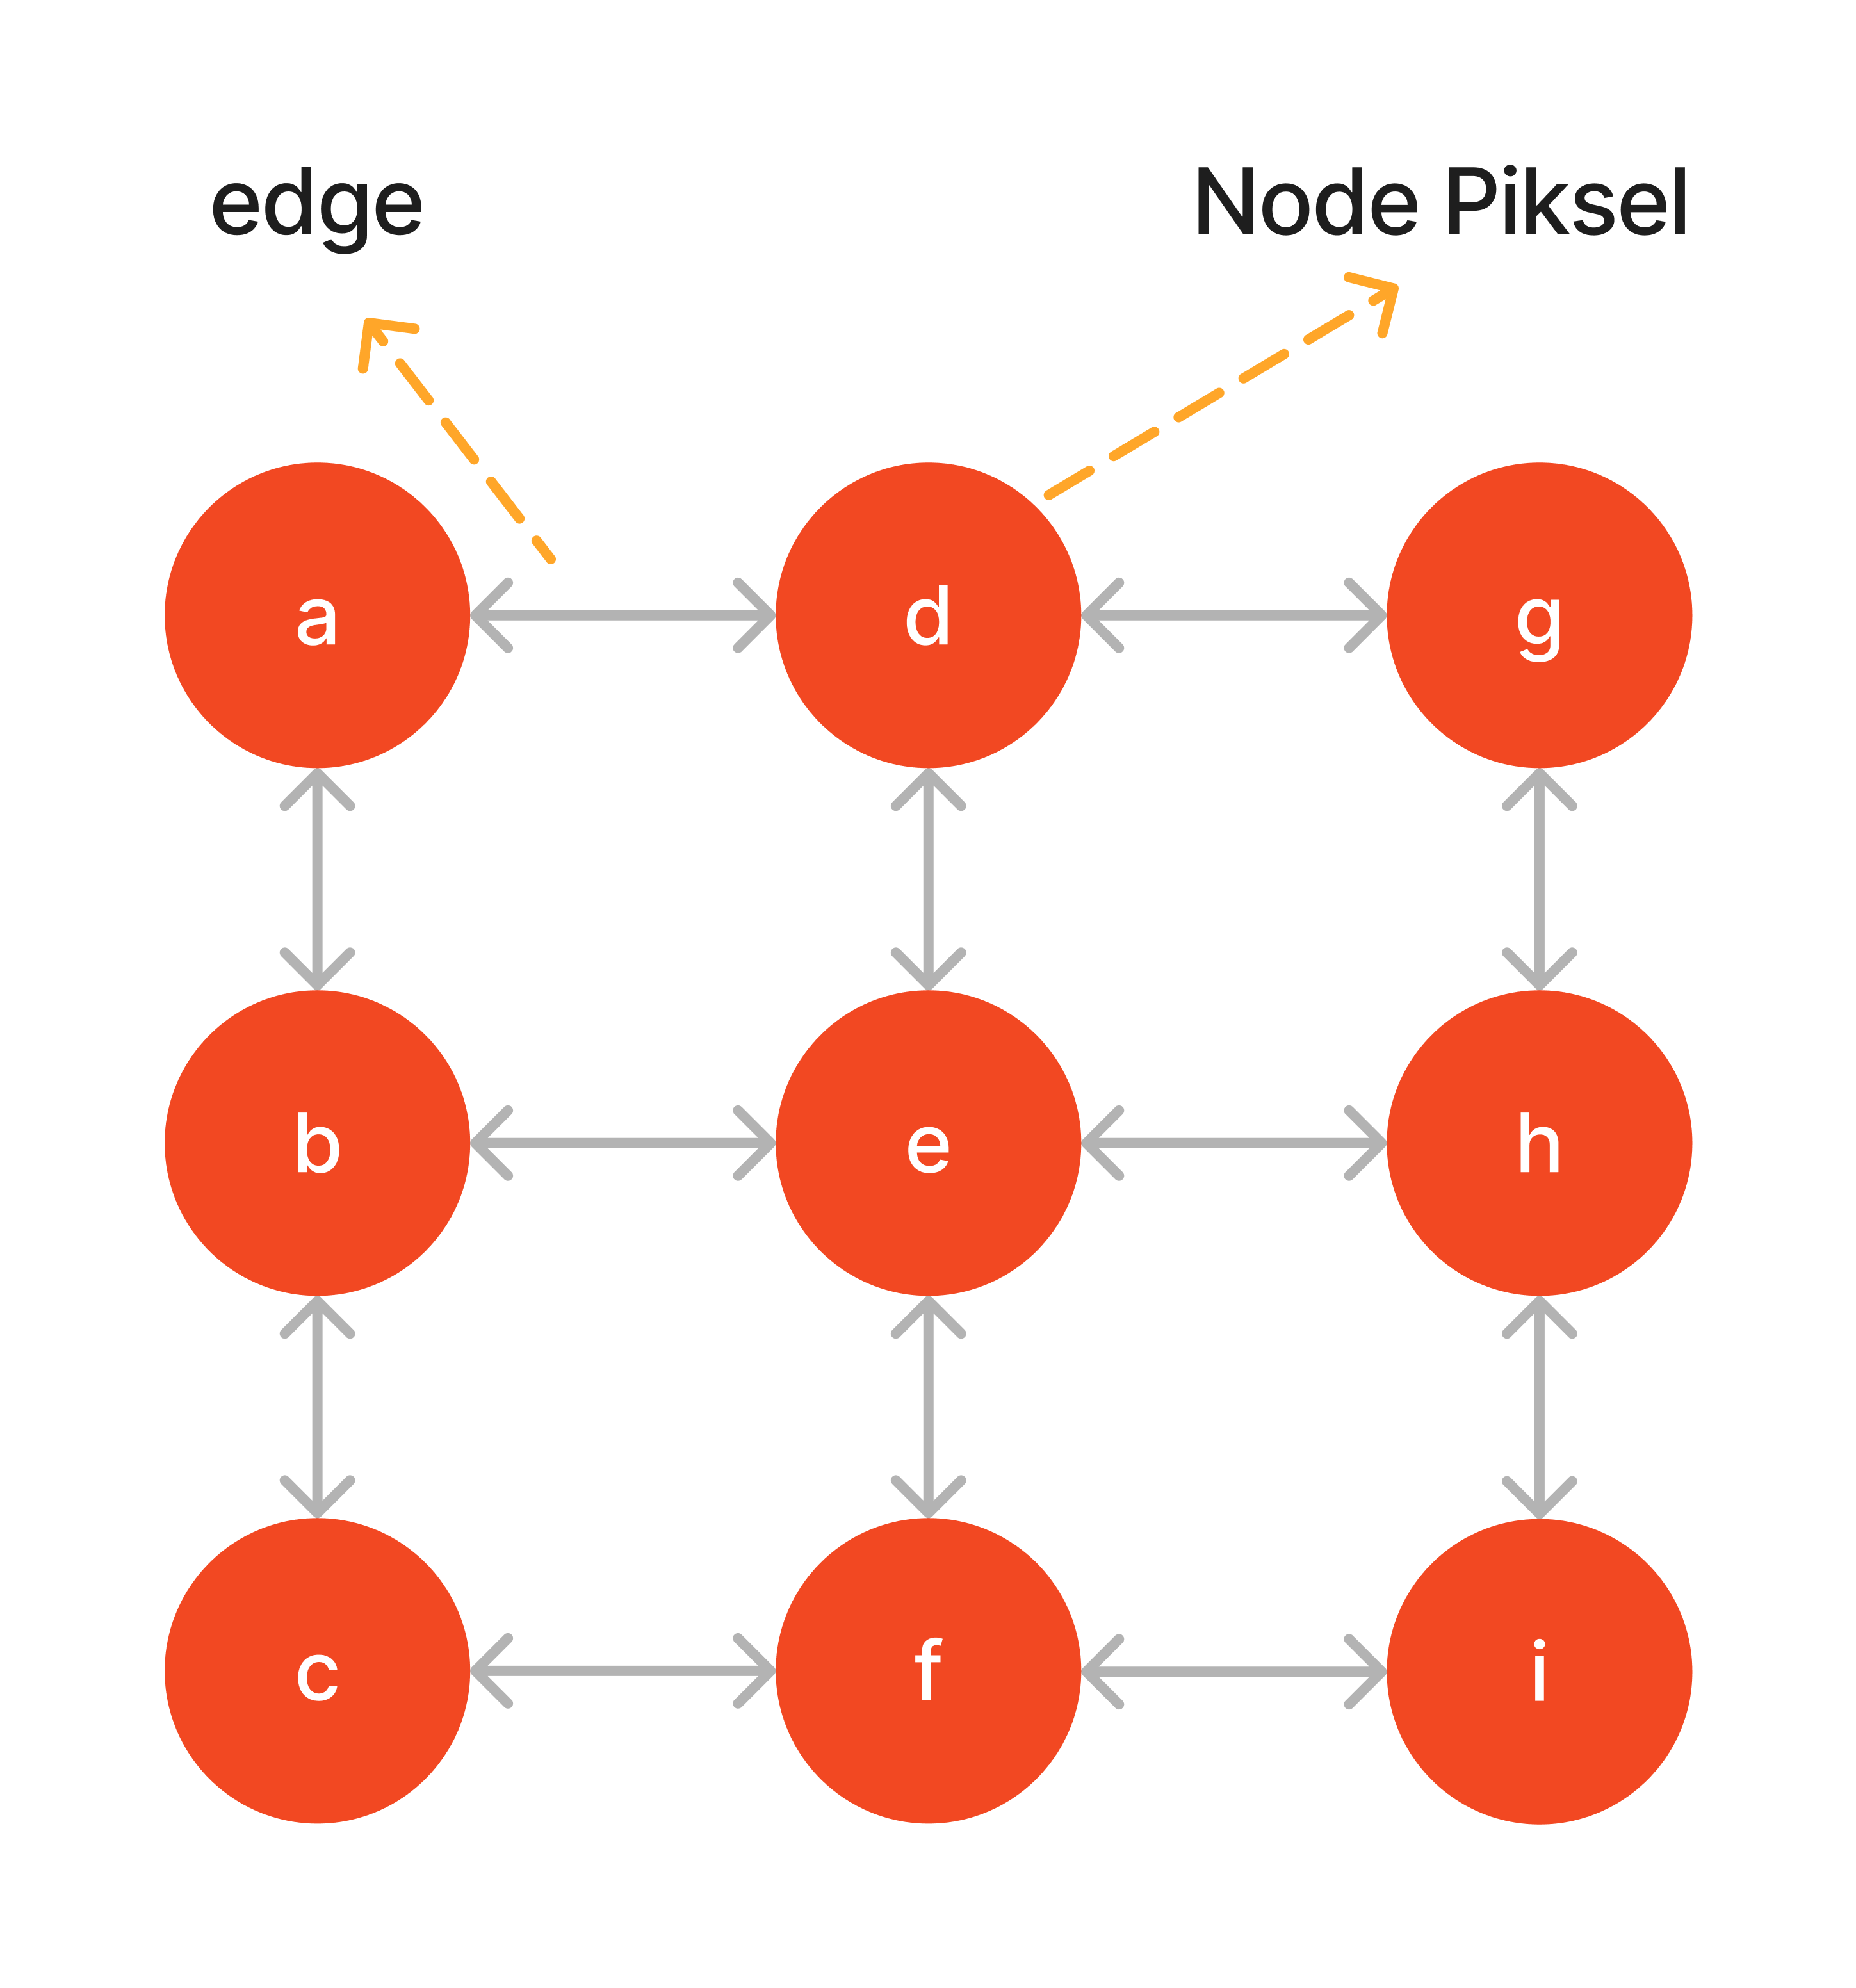
\includegraphics[width=0.3\textwidth]{gambar/graf.png}
	\caption{Ilustrasi graf terhadap piksel}
\end{figure}

Berikut struktur data untuk membangun graf
\begin{lstlisting} [language=C++, caption=Struktur data untuk membangun graf]

class Graph {
public:
    int num_nodes;
    vector<vector<int>> adj_list;

    // Constructor to initialize the graph with num_nodes vertices
    Graph(int num_nodes) {
        this->num_nodes = num_nodes;
        adj_list.resize(num_nodes);
    }

    // Function to add an edge between two vertices
    void add_edge(int u, int v) {
        adj_list[u].push_back(v);
        // adj_list[v].push_back(u); // If the graph is undirected
    }

    // Function to get edges of the graph
    vector<pair<int, int>> get_edges() {
        vector<pair<int, int>> edges;
        for (int u = 0; u < num_nodes; u++) {
            for (int v : adj_list[u]) {
                edges.push_back(make_pair(u, v));
            }
        }
        return edges;
    }
};
\end{lstlisting}
% int main() {
%     int num_nodes = 5; // Number of vertices in the graph
%     Graph graph(num_nodes);

%     // Adding edges to the graph
%     graph.add_edge(0, 1);
%     graph.add_edge(0, 4);
%     graph.add_edge(1, 2);
%     graph.add_edge(1, 3);
%     graph.add_edge(1, 4);
%     graph.add_edge(2, 3);
%     graph.add_edge(3, 4);

%     // Getting and printing the edges of the graph
%     vector<pair<int, int>> edges = graph.get_edges();
%     for (const auto& edge : edges) {
%         cout << edge.first << " -> " << edge.second << endl;
%     }

%     return 0;
% }

Setelah graf terbentuk, algoritma akan mulai mencari \emph{path} dari setiap \emph{node}
dengan ditentukannya dua \emph{node} khusus yaitu s (\emph{source}) dan t (\emph{sink}), 
dimana \emph{node} s akan menjadi  menjadi \emph{foreground} dan t menjadi \emph{background}.
Fungsi \emph{path} akan peneliti jelaskan pada bagian \ref{section:skenario_eksperimen}.

\begin{figure}[H]
	\centering{}
	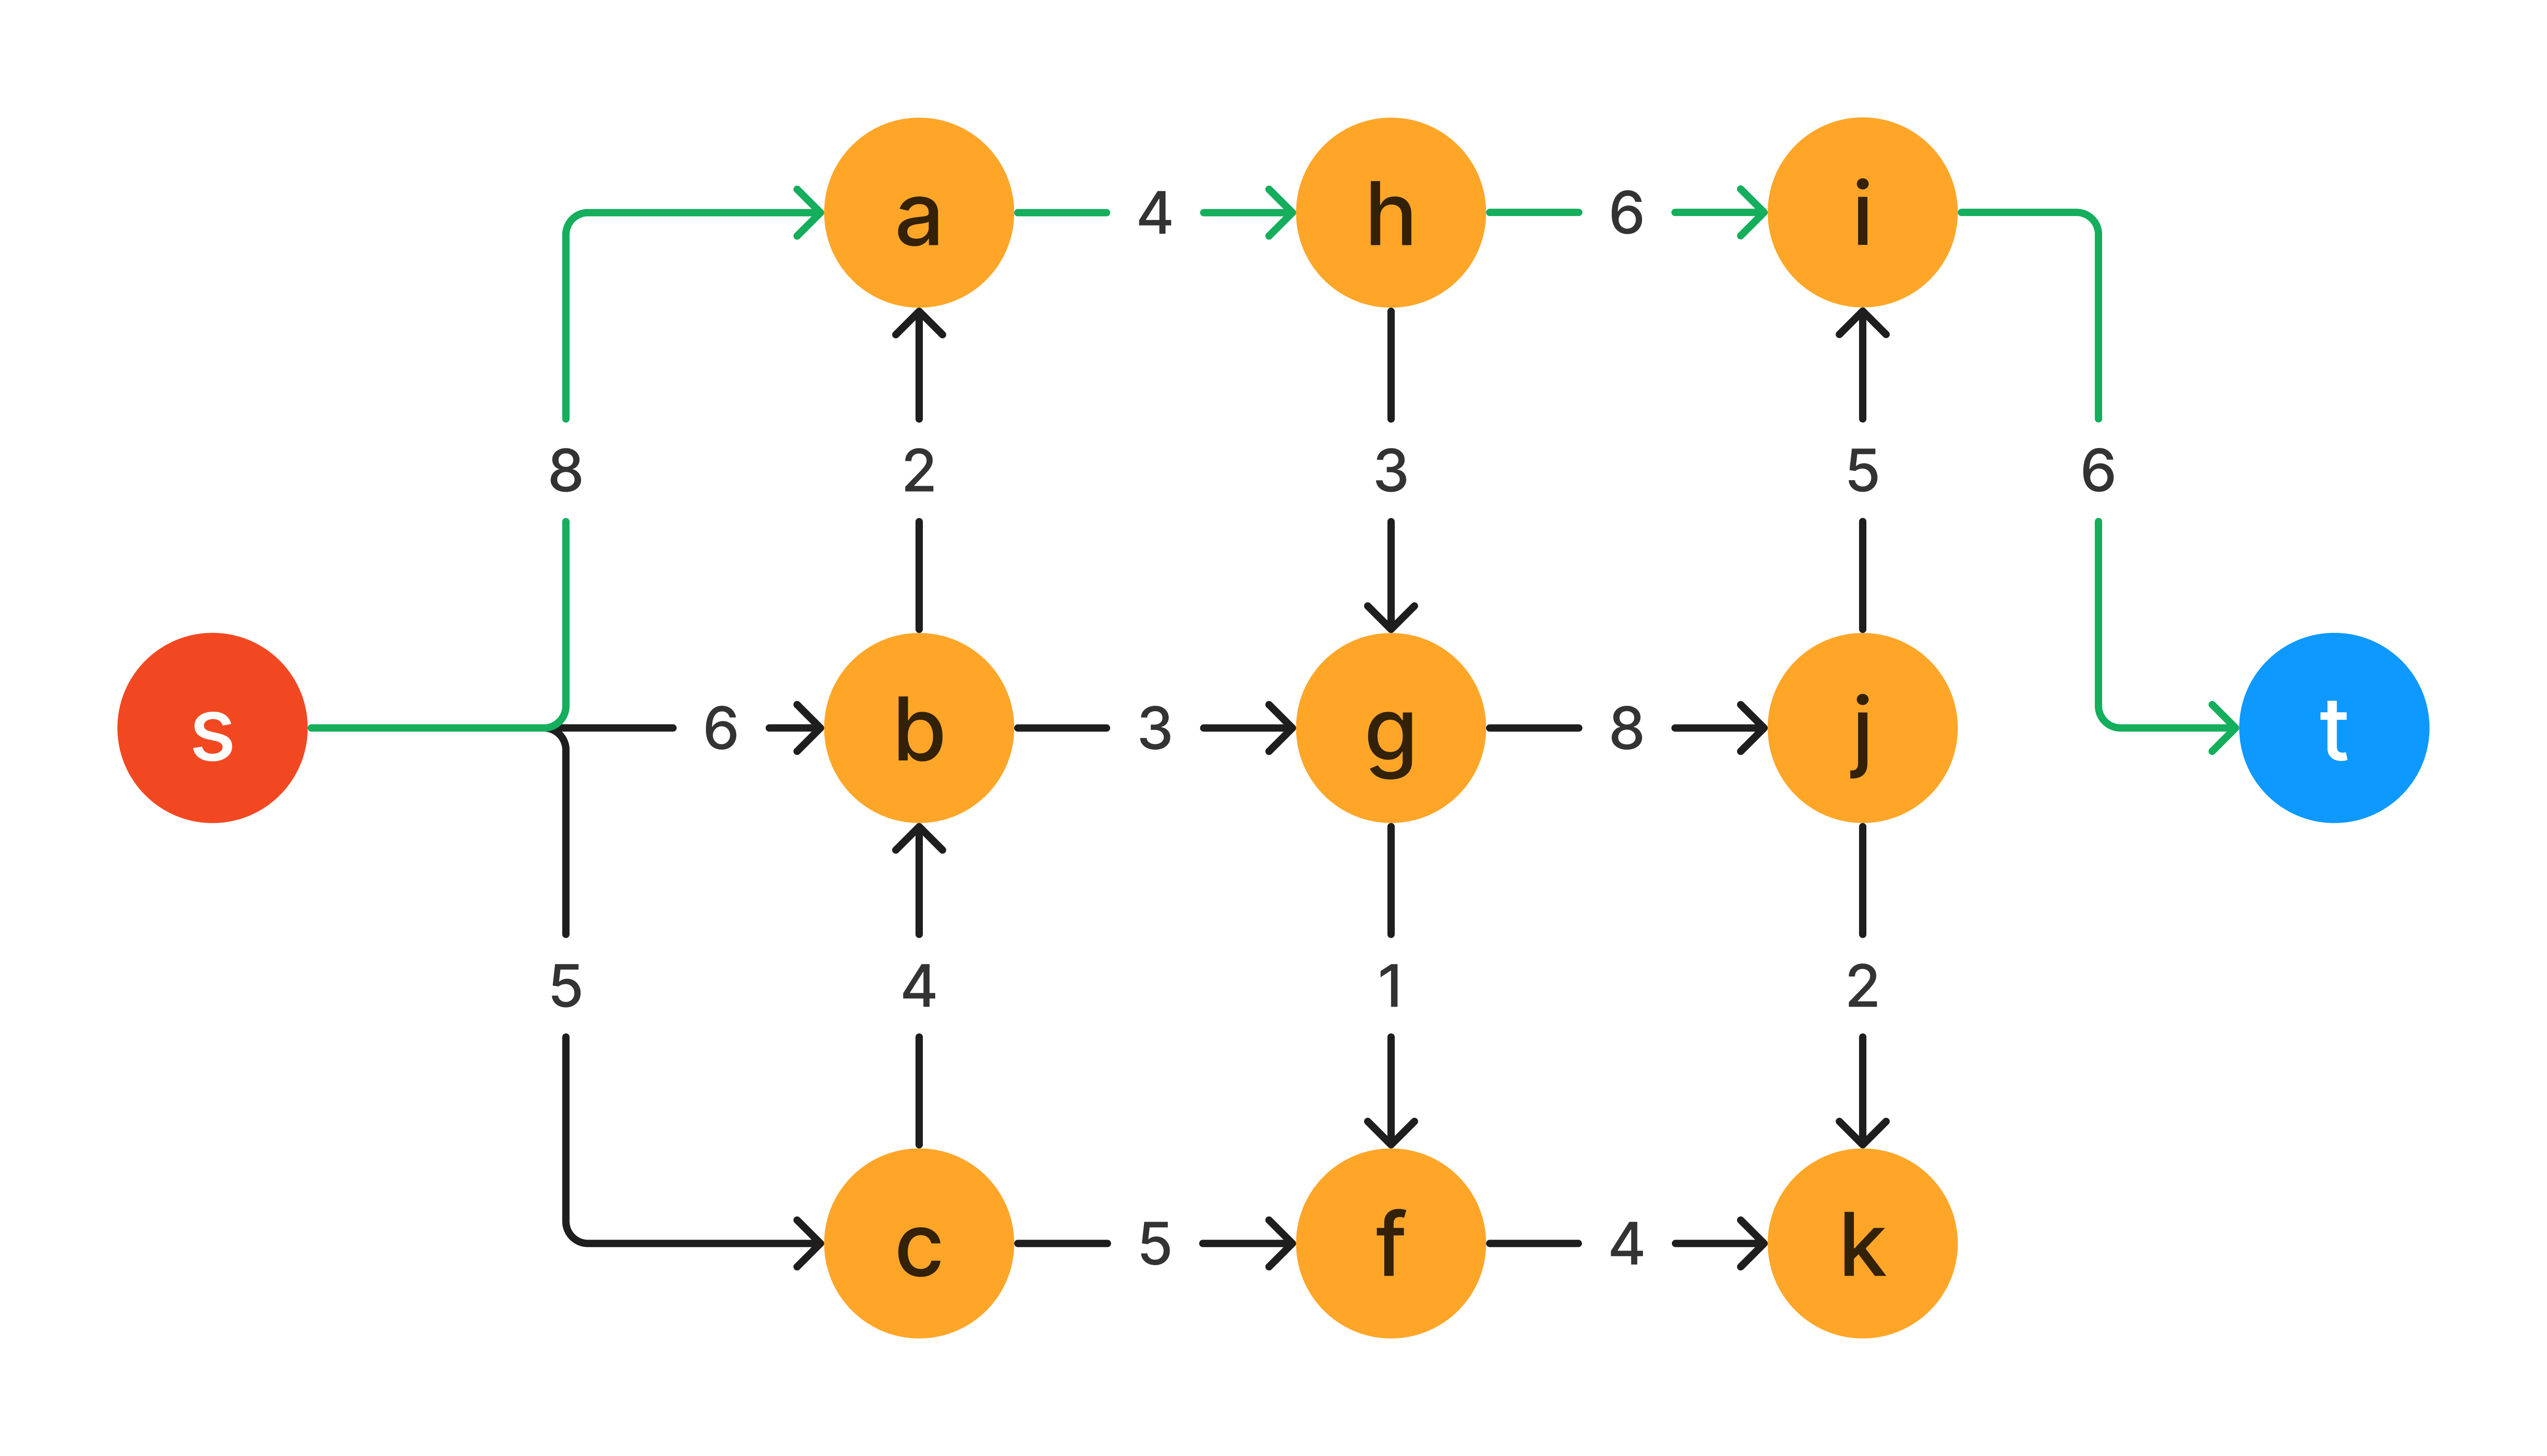
\includegraphics[width=0.6\textwidth]{gambar/contoh_path.png}
	\caption{Garis berwarna hijau menunjukkan \emph{path} s-a-h-i-t}
\end{figure}

% Berikut struktur data untuk mencari \emph{path}
% \begin{lstlisting} [language=C++, caption=Struktur data untuk mencari \emph{path}]

% class Node {
%     public:
%         char name;
%         int data;
%         int capacity; // Capacity of the edge between this node and its parent
%         Node* parent;
%         vector<Node*> children;
%         map<Node*, int> edges; // Map to store child nodes and their capacities


%         Node(char name) {
%             this->name = name;
%             parent = nullptr;
%             // capacity = 0; // Initialize capacity to 0
%         }
%     };

% class Tree {
%     private:
%         Node* root;
%     public:
%     Tree() {
%         root = nullptr;
%     }

%     void insertChild(Node* current, Node* next, int capacity) {
%         Node* rootOfCurrent = getRoot(current);
%         Node* rootOfNext = getRoot(next);

%         if(next->parent == nullptr || rootOfNext->name == rootOfCurrent->name){

%             next->parent = current;
%             current->edges[next] = capacity;
%             current->children.push_back(next);

%             // get root of each node
%             Node* nextRoot = getRoot(next);        
%             cout << "node " << next->name 
%             << " masuk ke tree " 
%             << nextRoot->name ;
%             cout << endl;

%         }else if (rootOfNext->name != rootOfCurrent->name){
%             cout << endl << "ada path di: "
%             << next->name << endl;
%             cout << "path nya adalah: "<< endl; 
%             getPath(current, next);
%             cout << "masuk ke tahap augmentasi" 
%             << endl << endl;
%         }  
        
%     }

%     // Add this helper function to get the capacity between two nodes
%     int getEdgeCapacity(Node* parent, Node* child) {
%         // Find the edge connecting the parent and child nodes
%         auto it = parent->edges.find(child);
%         if (it != parent->edges.end()) {
%             return it->second; // Return the capacity of the edge
%         }
%         return 0; // Return 0 if the edge is not found (should not happen if the tree is correctly constructed)
%     }
    

%     void display(Node* node, int depth = 0) {

%         if (node == nullptr)
%             return;

%         // Print current node with indentation
%         for (int i = 0; i < depth; ++i) {
%             cout << "    ";
%         }
%         cout << "|-- " << node->name << " (Capacity: " << node->capacity << ")" << endl;

%         // Recursively display children
%         for (Node* child : node->children) {
%             display(child, depth + 1);
%         }
%     }

%     void displayTree(Node* root) {
%         cout << endl << "Tree dari Search Node " 
%         << root->name << " adalah: " << endl;
%         display(root);
%     }

%     Node* getRoot(Node* child) {

%         Node* current = child;
%         while (current->parent != nullptr) {
%             current = current->parent;
%         }

%         return current;
%     }

%     vector<Node*> getLeafNodes(Node* node) {
%         vector<Node*> leafNodes;

%         if (node == nullptr){
%             return leafNodes;
%         }

%         if (node->children.empty()) {
%             leafNodes.push_back(node);
%         } else {
%             for (Node* child : node->children) {
%                 vector<Node*> childLeafNodes = 
%                 getLeafNodes(child);

%                 leafNodes.insert(
%                 leafNodes.end(), 
%                 childLeafNodes.begin(), 
%                 childLeafNodes.end()
%                 );
%             }
%         }        
%         return leafNodes;
%     }

%     void displayLeafNodes(Node* root) {
%         vector<Node*> leafNodes = getLeafNodes(root);
%         cout << "Leaf nodes: ";
%         for (Node* leafNode : leafNodes) {
%             cout << leafNode->name << " ";
%         }
%         cout << endl;
%     }
    
%     bool getPathToRoot(Node* leaf, 
%     vector<char>& path) {
%         if (leaf == nullptr)
%             return false;

%         Node* current = leaf;
%         while (current != nullptr) {
%             path.push_back(current->name);
%             current = current->parent;
%         }

%         return true;
%     }
    
%     vector<char> getPathFromLeafToRoot(Node* leaf) {
%         vector<char> path;
%         getPathToRoot(leaf, path);
%         return path;
%     }

%     void displayLeafToRoot ( Node* leaf) {
%         vector<char> path = 
%         getPathFromLeafToRoot(leaf);
%         getPathToRoot(leaf, path);

%         // Display the path
%         if(path[path.size()-1] != 't'){
%             reverse(path.begin(), path.end());
%         }
%         cout << "Path from leaf " << leaf->name 
%         << " to root:" << endl;
%         for (int i = 0; i < path.size(); i++) {
%             cout << path[i];
%             if(i != path.size() -1){
%                 cout<< "->";
%             }
%         }
%         cout << endl;
%     }

%     void getPath(Node* current, Node* next){
%         vector<char> tmp_current = 
%         getPathFromLeafToRoot(current);
%         vector<char> tmp_next = 
%         getPathFromLeafToRoot(next);
%         vector<char> path;
%         int totalCapacity = 0;

%         for (char cek : tmp_current){
%             cout<< cek ;
%         };

%         cout<<endl;

%         for (char cek2 : tmp_next){
%             cout<< cek2;
%         };

%         cout<< endl;



%         if(tmp_current[tmp_current.size() - 1] == 't'){

%             reverse(tmp_next.begin(), tmp_next.end());

%             for(char node : tmp_next){
%                 path.push_back(node);
%                 if (path.size() > 1) {
%                     Node* parent = next->parent;
%                     int capacity = getEdgeCapacity(parent, next);
%                     totalCapacity += capacity;
%                     cout << "Capacity from " << parent->name << " to " << next->name << ": " << capacity << endl;
%                 }
%             }
%             for(char node : tmp_current){
%                 path.push_back(node);
%                 if (path.size() > 1) {
%                     Node* parent = current->parent;
%                     int capacity = getEdgeCapacity(parent, current);
%                     totalCapacity += capacity;
%                     cout << "Capacity from " << parent->name << " to " << next->name << ": " << capacity << endl;
%                 }
%             }
%         }else{
            
%             reverse(tmp_current.begin(), tmp_current.end());

%             for(char node : tmp_current){
%                 path.push_back(node);
%                 if (path.size() > 1) {
%                     Node* parent = current->parent;
%                     int capacity = getEdgeCapacity(parent, current);
%                     totalCapacity += capacity;
%                     cout << "Capacity from cu " << parent->name << " to " << current->name << ": " << capacity << endl;
%                 }
%             }
%             for(char node : tmp_next){
%                 path.push_back(node);
%                 if (path.size() > 1 && next->parent != nullptr) {
%                     Node* parent_tmp = next->parent;
%                     // cout<< parent->name;
%                     int capacity = getEdgeCapacity(parent_tmp, next);
%                     totalCapacity += capacity;
%                     cout << "Capacity from ci " << parent_tmp->name << " to " << next->name << ": " << capacity << endl;
%                     next = parent_tmp;
%                 }
%             }
%         }
%         for (char i : path) {
%             cout << i;
%         }
%     }
% };
% \end{lstlisting}

% int main() {
% 	// Create Tree S and T
% 	Tree tree_S;
% 	Tree tree_T;
% 	// Create root node s and t
% 	Node* root_S = new Node('s');
% 	Node* root_T = new Node('t');

% 	Node* nodeA = new Node('a');
% 	Node* nodeB = new Node('b');
% 	Node* nodeC = new Node('c');
% 	Node* nodeH = new Node('h');
% 	Node* nodeG = new Node('g');
% 	Node* nodeF = new Node('f');
% 	Node* nodeI = new Node('i');
% 	Node* nodeJ = new Node('j');

% 	tree_S.insertChild(root_S, nodeA);
% 	tree_S.insertChild(root_S, nodeB);
% 	tree_S.insertChild(root_S, nodeC);
% 	tree_T.insertChild(root_T, nodeI);
% 	tree_S.insertChild(nodeA, nodeH);
% 	tree_S.insertChild(nodeB, nodeG);
% 	tree_S.insertChild(nodeC, nodeF);
% 	tree_T.insertChild(nodeI, nodeH);
% 	tree_T.insertChild(nodeI, nodeJ);
%    return 0;
% }

\subsection{Algoritma \emph{GrabCut}}
Struktur data penelitian algoritma \emph{GrabCut} pada penelitian kali ini sebagai 
sebagai berikut: 

\begin{lstlisting} [language=C++, caption=Struktur data GrabCut]
// Struktur Data GrabCut
#include <iostream>
#include <opencv2/core/core.hpp>
#include <opencv2/highgui/highgui.hpp>
#include <boost/numeric/ublas/matrix.hpp>
#include <boost/numeric/ublas/vector.hpp>
#include <vector>
#include <algorithm>
#include <numeric>
#include <cmath>
#include <map>

class GrabCut {
private:
    cv::Mat gambar;
    int rows, cols;
    cv::Mat gambar_mask;
    int komponen_gmm;
    int nilai_gamma;
    int nilai_beta;

public:
    GrabCut(const cv::Mat& gambar, const cv::Mat& gambar_mask, int rect[4] = nullptr, int komponen_gmm = 5) {
        this->gambar = gambar;
        this->rows = gambar.rows;
        this->cols = gambar.cols;
        this->gambar_mask = gambar_mask;
        this->komponen_gmm = komponen_gmm;
        this->nilai_gamma = 50;
        this->nilai_beta = 0;
    }

    void inisiasi_piksel(){}
    void init_assign_gmm(){}
    void memperbarui_gmm(){}
    void hitung_smoothness(){}
    void bangun_graf(){}
    void mincut_segmentation(){}
};

class GaussianMixture {
private:
    int komponen_gmm;
    int jumlah_fitur;
    vector<int> jumlah_sampel;
    ublas::vector<double> coefs;
    ublas::matrix<double> means;
    ublas::matrix<double> covariances;

public:
    GaussianMixture(const ublas::matrix<double>& X, int komponen_gmm = 5) {
        this->komponen_gmm = komponen_gmm;
        this->jumlah_fitur = x[1].size();
        this->jumlah_sampel = ublas::zero_vector<double>(komponen_gmm);

        this->coefs = ublas::zero_vector<double>(komponen_gmm);
        this->means = ublas::zero_matrix<double>(komponen_gmm, jumlah_fitur);
        this->covariances = ublas::zero_matrix<double>(komponen_gmm, jumlah_fitur * jumlah_fitur);
    }

    void init_rand(){}
    void dis_mult(){}
    void prob_calc(){}
    void learn_gmm(){}
    void count_params(){}
}

class mincut_segmentation {
public:
    void build_graph(){}
    void run(){}
    void growth(){}
    void augmentation(){}
    void adoption(){}
}
\end{lstlisting}

\section{Algoritma Segmentasi Gambar dengan Metode \emph{GrabCut}}

Algoritma \emph{GrabCut} terdiri dari gabungan beberapa algoritma lain, yaitu 
pemrosesan oleh algoritma GMM dan minimisasi energi oleh algoritma \emph{GraphCut},
berikut algoritma dari \emph{GrabCut}:  

\begin{algorithm}                     
\caption{Algoritma segmentasi gambar dengan \emph{GrabCut} (\cite{Rother:2004})}          
\label{algo:grabcut}                          
\begin{algorithmic}                    % enter the algorithmic environment
    % \State $\textbf{From \xspace} GaussianMixtureModels \textbf{\xspace Import \xspace} GaussianMixture$
    \State $gambar \gets \Call{loadImage}$  \Comment{Input gambar 2.jpg}
    \State $\textbf{bool } kotak \gets false$ \Comment{Inisiasi keberadaan kotak}
    \State $\textbf{bool } drawing \gets false$ \Comment{Inisiasi keberadaan brush}
    \State $iy, ix \gets int$
    \State $gambar2 \gets \Call{Copy}{gambar}$
    \State $mask \gets \Call{ublas::zero\textunderscore matrix<double>}{gambar.shape[0], gambar.shape[1]}$
    \State $map<string, string> flagsColor$
    \State $map<string, integer> flagsValue$
    
    \State $flagsColor['bg'], flagsColor['fg']  \gets 'black', 'white'$
    \State $flagsValue['bg'], flagsValue['fg'], flagsValue['prob\textunderscore bg'], flagsValue['prob\textunderscore fg'] \newline
     \gets 0, 1, 2, 3$
    
    \\
    % GrabCut Class
    \State $komponen\textunderscore piksel \gets \newline
    \hspace*{2em} \Call{ublas::zero\textunderscore matrix<double>}{gambar.shape[0], gambar.shape[1]}$
    \State $\textbf{array } kotak\textunderscore lok[4] \gets [...]$
    % \State $flagsValue['bg'] \gets 0$
    % \State $flagsValue['prob\textunderscore bg'] \gets 2$
    % \State $flagsValue['prob\textunderscore fg'] \gets 3$

    % \State $flags['bg'] \gets ['black', 0]$
    % \State $flags['fg'] \gets ['white', 1]$
    % \State $flags['pr\textunderscore bg'] \gets ['red', 2]$
    % \State $flags['pr\textunderscore fg'] \gets ['blue', 3]$
    \\
    \Function{MouseHandler}{$event, x, y, flagsColor, flagsValue, param$}
        \If{$event == \Call{cv}{EVENT\textunderscore RBUTTON}$} 
            \State $ix, iy = x, y$
            \State $\Call{cv.rectangle}{gambar, (ix, iy), (x, y), flagsColor['warna'], 2}$
            \State $kotak \gets True$
            \State $kotak\textunderscore lok[4] \gets [min(ix, x), min(iy, y), abs(ix-x), abs(iy-y)]$
        \EndIf 
        \If{$event == \Call{cv}{EVENT\textunderscore LBUTTON}$} 
            \State $drawing \gets True$
            \State $\Call{cv.circle}{gambar, (x, y), 3, flagsColor['warna'], -1}$
            \State $\Call{cv.circle}{mask, (x, y), 3, flagsValue['value'], -1}$
            \State $drawing \gets False$
        \EndIf 
    \EndFunction
    \\
\algstore{algo:algo_all}
\end{algorithmic}
\end{algorithm}

\begin{algorithm}                     
\begin{algorithmic}                    % lanjutan algo_all di atas
\algrestore{algo:algo_all}

    \\
    \Comment{\textbf{ (Algorithm \ref{algo:intialize}) } Inisiasi TU = 1 untuk piksel didalam kotak, gambar \ref{gambar:2.6} }

    \Function{inisasi\textunderscore piksel}{$mask$}
        \If{$kotak\textunderscore lok[4] \neq None $} 
            \State $mask[kotak\textunderscore lok[...]] = 1$ 
        \EndIf
        \State $idx\textunderscore bg \gets bg['value'] \textbf{ or } pr\textunderscore bg['value']$
        \State $idx\textunderscore fg \gets fg['value'] \textbf{ or } pr\textunderscore fg['value']$
    \EndFunction

    \\ 
    \Comment{\textbf{ (Algorithm \ref{algo:assign_GMM}) } Inisiasi dan \emph{Assign} GMM ke setiap piksel, tahap 1 gambar \ref{gambar:2.6} }
    \Function{init\textunderscore assign\textunderscore gmm}{$idx\textunderscore bg, idx\textunderscore fg$}
        \State $GMM\textunderscore FG \gets GaussianMixture(idx\textunderscore fg)$
        \State $GMM\textunderscore BG \gets GaussianMixture(idx\textunderscore bg)$
        \State $\Call{GMM\textunderscore FG.dis\textunderscore mult}{idx\textunderscore fg}$
        \State $\Call{GMM\textunderscore BG.dis\textunderscore mult}{idx\textunderscore bg}$
    \EndFunction

    \\ 
    \Comment{\textbf{ (Algorithm \ref{algo:learn_GMM}) } mempelajari parameter GMM, tahap 2 gambar \ref{gambar:2.6} }
    \Function{memperbarui\textunderscore gmm}{}
        \State $\Call{GMM\textunderscore FG.count\textunderscore params}{gambar[idx\textunderscore fg], komponen\textunderscore piksel[idx\textunderscore fg]}$
        \State $\Call{GMM\textunderscore BG.count\textunderscore params}{gambar[idx\textunderscore bg], komponen\textunderscore piksel[idx\textunderscore bg]}$
    \EndFunction

    \\ 
    \Comment{\textbf{ (Algorithm \ref{algo:mincut_algorithm}) } segmentasi piksel, tahap 3 gambar \ref{gambar:2.6} }
    \Function{gc\textunderscore segmentation}{}
        \State $\textbf{vector<int> } gc\textunderscore graph \gets \Call{build\textunderscore graph}{edges, n\textunderscore piksel}$
        \State $\Call{mincut\textunderscore segmentation}{gc\textunderscore graph, gc\textunderscore sink, gc\textunderscore source, gc\textunderscore graph\textunderscore capacity}$
    \EndFunction
\end{algorithmic}
\end{algorithm}

\begin{algorithm}                     
    \caption{Algoritma inisialisasi \emph{bounding box} pada area luka}          
    \label{algo:intialize}                          
    \begin{algorithmic}                    % enter the algorithmic environment
        \\  \Comment{Tahap inisialisasi pada gambar \ref{gambar:2.6}}
    
        \Function{inisasi\textunderscore piksel}{$mask$}

            \If {$kotak\textunderscore lok \neq None$}
                \State $mask[kotak\textunderscore lok[1]:kotak\textunderscore lok[1] + 
                kotak\textunderscore lok[3],\newline  
                \hspace*{4em} kotak\textunderscore lok[0]: kotak\textunderscore lok[0] + 
                kotak\textunderscore lok[2]] \gets flags['fg']['value']$
            \EndIf

            \State $idx\textunderscore bg \gets \textbf{where}(mask == flags['bg']['value']  \textbf{\xspace or\xspace}  \newline 
            \hspace*{4em} mask == flags['pr\textunderscore bg']['value'])$
            \State $idx\textunderscore fg \gets \textbf{where}(mask == flags['fg']['value']  \textbf{\xspace or\xspace}  \newline 
            \hspace*{4em} mask == flags[''pr\textunderscore fg']['value'])$
        
        \EndFunction
    % \algstore{algo:initialize}
    \end{algorithmic}
\end{algorithm}
        

\begin{algorithm}                     
    \caption{Algoritma inisiasi dan \emph{Assign} GMM pada setiap piksel citra}          
    \label{algo:assign_GMM}                          
    \begin{algorithmic}                    % enter the algorithmic environment

    \State $typedef ublas::matrix<double> Matrix;$
    \State $typedef ublas::vector<double> Vector;$

    \Function{init\textunderscore assign\textunderscore gmm}{$idx\textunderscore bg, idx\textunderscore fg$}
        \State $GMM\textunderscore BG \gets GaussianMixture(gambar[idx\textunderscore bg])$
        \State $GMM\textunderscore FG \gets GaussianMixture(gambar[idx\textunderscore fg])$

        \State $komponen\textunderscore piksel[idx\textunderscore bg] \gets \Call{GMM\textunderscore BG.dis\textunderscore mult}{gambar[idx\textunderscore bg]}$
        \State $komponen\textunderscore piksel[idx\textunderscore fg] \gets \Call{GMM\textunderscore FG.dis\textunderscore mult}{gambar[idx\textunderscore fg]}$
    \EndFunction
    \\
    \Function{dis\textunderscore mult}{$target$} \Comment{rumus \ref{eq:distribusi_multi}}
        \State $gauss\textunderscore score \gets  \Call{np.zeros}{target.shape[0]}$
        \State $\Call{init\textunderscore rand}{$target$}$
        \For{$k = 0; k < komponen\textunderscore gmm; k++$}
            \If{$coefs > 0$}
                \State $Vector XminMu \gets target - means[k]$
                \State $Vector trans\textunderscore XminMu \gets \Call{ublas::trans}{XminMu}$
                \State $Matrix inv\textunderscore cov = ublas::inv(self.covariances[ci])$
                \State $tmp\textunderscore dot \gets \Call{ublas::prod}{inv_cov, trans\textunderscore XminMu}$
                \State $tmp\textunderscore mult \gets \Call{ublas::element\textunderscore prod}{'ij,ij->i', \newline 
                \hspace*{6em} XminMu, ublas::trans(tmp\textunderscore dot)}$
                \State $pembagi \gets \Call{sqrt}{2* M.PI} * \Call{sqrt}{ublas::det(covarians[k])}$
                \State $gauss\textunderscore score \gets \frac{\Call{np.exp}{-0.5 * tmp\textunderscore mult}}{pembagi}$
            \EndIf
        \EndFor
        \State $\textbf{return } \Call{np.argmax}{gauss\textunderscore score}$
    \EndFunction
    \\
    \Function{init\textunderscore rand}{$target$}
        \State $\textbf{vector<int> } labelPix[target.shape[0]]$
        \For{$\textbf{int } i = 0; i < target.shape[0]; i++$}
            \State $labelPix[i] \gets rand() \mod 5;$
        \EndFor
        \State $\Call{count\textunderscore params}{target, labelPix}$
    \EndFunction
    \end{algorithmic}
\end{algorithm}

\begin{algorithm}
    \caption{Algoritma mempelajari parameter GMM}          
    \label{algo:learn_GMM}                 
    \begin{algorithmic}            % enter the algorithmic environment
        \\  \Comment{Tahap mempelajari GMM \ref{gambar:2.6}}
        \State $vector<int> unique\textunderscore labels;$
        \State $vector<int> labelCounts;$
    
        \Function{memperbarui\textunderscore GMM}{}
            \State $\Call{count\textunderscore params}{gambar[idx\textunderscore bg], komponen\textunderscore piksel[idx\textunderscore bg]} $
            \State $\Call{count\textunderscore params}{gambar[idx\textunderscore fg], komponen\textunderscore piksel[idx\textunderscore fg]} $
        \EndFunction

        \Function{count\textunderscore params}{$ublas::matrix<double> target,\newline 
        \hspace*{4em} ublas::matrix<double> labels$}
            \State $tie(unique\textunderscore labels, labelCounts) = uniqueWithCounts(labels);$

            \For{\textbf{int }k = 0; k < unique\textunderscore labels; k++}
                % \State $\textbf{int }n\textunderscore k\textunderscore idx \gets labelCounts[k]$
                \State $coefs[k] \gets labelCounts[k] / accumulate(labelCounts.begin(), labelCounts.end(), 0)$
                \State $means[k] \gets ublas::mean(target[k == labels])$
                \State $covariances[k] \gets ublas::trans(ublas::cov(target[k == labels]))$
            \EndFor
        \EndFunction

        \\ \Comment{Fungsi untuk mencari nilai unik k tiap piksel}
        \Function{$pair<vector<int>, vector<int>> \newline search\textunderscore uniques$}{$const ublas::matrix<double>\& labels$} 
            \State $vector<int> unique\textunderscore labels;$
            \State $vector<int> labelCounts;$
            \State $map<int, int> countMap;$
        
            \\ \Comment{Menghitung jumlah muncul nilai k}
            \For{const auto\& label : labels}
                \State $countMap[label]++;$
            \EndFor
        
            \\ \Comment{Memisahkan nilai unik dan jumlah kemunculannya}
            \For{const auto\& entry : countMap}
                \State $unique\textunderscore labels.push\textunderscore back(entry.first);$
                \State $labelCounts.push\textunderscore back(entry.second);$
            \EndFor
        
            \State $\textbf{return } make\textunderscore pair(unique\textunderscore labels, labelCounts);$
        \EndFunction
    \end{algorithmic}
\end{algorithm}

\begin{algorithm}
    \caption{Algoritma segmentasi oleh \emph{mincut}}          
    \label{algo:mincut_algorithm}                 
    \begin{algorithmic}            % enter the algorithmic environment
        \State $\textbf{vector<int> } edges$
        \State $\textbf{vector<double> } D\textunderscore score$
        \State $\textbf{vector<int> } gc\textunderscore graph\textunderscore capacity$
        \State $\textbf{int } n\textunderscore piksel \gets gambar.shape[0] * gambar.shape[1]$
        \State $\textbf{int } gc\textunderscore source \gets n\textunderscore piksel$
        \State $\textbf{int } gc\textunderscore sink \gets gc\textunderscore source + 1$

        \Function{$gc\textunderscore segmentation$}{$\textbf{vector<int> } edges, \textbf{int } n\textunderscore piksel$}  
            \State $\textbf{vector<int> } gc\textunderscore graph \gets \Call{build\textunderscore graph}{edges, n\textunderscore piksel}$
            \State $\Call{mincut\textunderscore segmentation}{gc\textunderscore graph, gc\textunderscore sink, gc\textunderscore source, gc\textunderscore graph\textunderscore capacity}$
        \EndFunction
    \end{algorithmic}
\end{algorithm}

\begin{algorithm}
    \caption{Membangun graf}          
    \label{algo:build_graph}                 
    \begin{algorithmic}            % enter the algorithmic environment
        \\  \Comment{Tahap membangun graf }

        \State $\textbf{vector<int> } idx\textunderscore bg \gets np.where(mask.reshape(-1) == flagsValue['bg'])$
        \State $\textbf{vector<int> } idx\textunderscore fg \gets np.where(mask.reshape(-1) == flagsValue['fg'])$
        \State $\textbf{vector<int> } idx\textunderscore pr \gets np.where(mask.reshape(-1) == flagsValue['prob\textunderscore bg'] 
        \textbf{ or } mask.reshape(-1) == flagsValue['prob\textunderscore fg'])$

        \Function{$build\textunderscore graph$}{$\textbf{vector<int> } edges, \textbf{int } n\textunderscore piksel$}  
        \State $\textbf{Graph } graph\textunderscore gc((n\textunderscore piksel + 2))$
        % \\
        % \\ \Comment{Membangun graf untuk \emph{t-links}}
            \For{\textbf{int } i in (idx\textunderscore bg[0], idx\textunderscore fg[0], idx\textunderscore pr[0])}
                \State $\Call{graph\textunderscore gc.add\textunderscore edge}{gc\textunderscore source, i}$
                \State $\Call{graph\textunderscore gc.add\textunderscore edge}{gc\textunderscore sink, i}$
                \State $D\textunderscore score = -np.log(GMM\textunderscore BG \textbf{ or } GMM\textunderscore FG \newline
                \hspace*{8em} .count\textunderscore prob(gambar.reshape(-1, 3)[idx\textunderscore pr]))$
            \EndFor
            \State $\Call{gc\textunderscore graph\textunderscore capacity.push\textunderscore back}{(D\textunderscore score)} $
        \EndFunction
    \end{algorithmic}
\end{algorithm}

\begin{algorithm}
    \caption{Menghitung nilai D pada rumus \ref{eq:rumus_energi2}}          
    \label{algo:count_prob}                 
    \begin{algorithmic}            % enter the algorithmic environment
        \State $\textbf{vector<double> } prob$
        \Function{$count\textunderscore prob$}{$\textbf{vector<int> } target$}  
            \State $prob \gets [\Call{dis\textunderscore mult}{target}]$
            \State $\textbf{return } ublas::dot(coefs, prob)$
        \EndFunction
    \end{algorithmic}
\end{algorithm}

\begin{algorithm}
    \caption{Segmentasi oleh algoritma \emph{mincut} \ref{gambar:2.6}}          
    \label{algo:mincut_segmentation}                 
    \begin{algorithmic}            % enter the algorithmic environment
        \\ \Comment{Inisialiasi A, Path, dan O}
        \State $\textbf{vector<Node*> }  active\textunderscore nodes$
        \State $\textbf{vector<Node*> }  orphans\textunderscore nodes$
        \State $\textbf{vector<Node*> }  paths \gets null$
        \State $\textbf{vector<double> } tree\textunderscore cap$


        \\ \Comment{Inisialiasi S dan T}
        \State $\textbf{Tree }  tree\textunderscore S$
        \State $\textbf{Tree }  tree\textunderscore T$
        \State $\textbf{Tree }  tree$
        

        \State $\textbf{Node*} root\textunderscore S \gets \textbf{new} Node(gc\textunderscore source)$
        \State $\textbf{Node*} root\textunderscore T \gets \textbf{new} Node(gc\textunderscore sink)$
        \State $active\textunderscore nodes \gets \Call{active\textunderscore nodes.push\textunderscore back}{gc\textunderscore source, gc\textunderscore sink}$
        % \State $$

        \Function{$mincut\textunderscore segmentataion$}{$\textbf{vector<int> } gc\textunderscore graph, gc\textunderscore sink, gc\textunderscore source, gc\textunderscore graph\textunderscore capacity$}  
            \While{$true$}
                \State $\Call{growth\textunderscore step()}{}$
                \If{$paths \neq 0$}
                    \State $\Call{augmentation\textunderscore step(gc\textunderscore sink, gc\textunderscore source)}{}$
                \EndIf
                \State $\Call{adoption\textunderscore step(gc\textunderscore sink, gc\textunderscore source)}{}$

                % \For{$...$}
                %     \State $...$
                % \EndFor
            \EndWhile
        \EndFunction
    \end{algorithmic}
\end{algorithm}

% \begin{algorithm}
%     \caption{tahap growth pada \emph{mincut} di bagian \ref{fase_growth}}          
%     \label{algo:fase_growth}                 
%     \begin{algorithmic}            % enter the algorithmic environment
%         \Function{$growth\textunderscore step$}{}
%             \State $\textbf{vector<Node*> } list\textunderscore neighbors $
%             \State $\Call{search\textunderscore neighbors}{active\textunderscore nodes, tree\textunderscore cap}$
%             \While{$active\textunderscore nodes \neq 0$}
%                 \For{$\textbf{int }i; i < list\textunderscore neighbors.size(); i++$}
%                     \If{$tree\textunderscore cap[i] > 0$}
%                         \If{$\textbf{tree.getRoot}(list\textunderscore neighbors[i]) == null$}
%                             \State $tree.insertChild(active\textunderscore nodes[0], list\textunderscore neighbors[i])$
%                         \ElsIf{$\textbf{tree.getRoot}(list\textunderscore neighbors[i]) \neq null \textbf{ and } \newline
%                                 \textbf{tree.getRoot}(list\textunderscore neighbors[i]) \neq \textbf{tree.getRoot}(active\textunderscore nodes[0])$}
%                             \State $paths \gets tree.getPath(active\textunderscore nodes[0], list\textunderscore neighbors[i])$                    
%                         \EndIf
%                     \EndIf
%                 \EndFor
%                 \State $active\textunderscore nodes.pop()$
%             \EndWhile
%             \State $\textbf{return } paths \neq 0$
%         \EndFunction
%     \end{algorithmic}
% \end{algorithm}

% \begin{algorithm}
%     \caption{tahap augmentasi pada \emph{mincut} di bagian \ref{fase_augmentation}}          
%     \label{algo:fase_augmentation}                 
%     \begin{algorithmic}            % enter the algorithmic environment
%         \Function{$augmentation\textunderscore step$}{$\textbf{vector<int> } gc\textunderscore graph, gc\textunderscore sink, gc\textunderscore source$}
%             \Call{$tree.get\textunderscore residu$}{paths, gc\textunderscore graph\textunderscore capacity}
%             \For{$\textbf{int }i; i < path\textunderscore residu.size(); i++$}
%                 \If{$\textbf{tree.getRoot}(i[0]) == \textbf{tree.getRoot}(i[1]) == gc\textunderscore source$}
%                     \State $\textbf{tree.setParentNull}(i[1])$
%                     \State $orphans.push\textunderscore back(i[1])$
%                 \ElsIf{$\textbf{tree.getRoot}(i[0]) == \textbf{tree.getRoot}(i[1]) == gc\textunderscore sink$}
%                     \State $\textbf{tree.setParentNull}(i[0])$
%                     \State $orphans.push\textunderscore back(i[0])$
%                 \EndIf
%             \EndFor
%         \EndFunction
%     \end{algorithmic}
% \end{algorithm}

% \begin{algorithm}
%     \caption{tahap augmentasi pada \emph{mincut} di bagian \ref{fase_adoption}}          
%     \label{algo:fase_adoption}                 
%     \begin{algorithmic}            % enter the algorithmic environment
%         \Function{$adoption\textunderscore step$}{$\textbf{vector<int> } gc\textunderscore graph, gc\textunderscore sink, gc\textunderscore source$}
%             \State $\textbf{Node*} current\textunderscore orphans $
%             \While{$orphans \neq 0$}
%                 \State $current\textunderscore orphans \gets orphans[0]$
%                 \State $\Call{search\textunderscore neighbors}{current\textunderscore orphans, tree\textunderscore cap}$
%                 \State $orphans.pop()$
%                 \For{$\textbf{int }i; i < list\textunderscore neighbors.size(); i++$}
%                     \If{$tree.getRoot(list\textunderscore neighbors[i]) == \hfill \newline 
%                     \hspace*{5em} tree.getRoot(current\textunderscore orphans)  \textbf{ and } \hfill \newline 
%                     \hspace*{5em} tree.getEdgeCapacity(list\textunderscore neighbors[i],\newline 
%                     \hspace*{5em} current\textunderscore orphans) > 0$} 
%                         \State $tree.insertChild(list\textunderscore neighbors[i], current\textunderscore orphans)$     
%                         \State $\textbf{break}$             
%                     \EndIf 
%                 \EndFor
%             \EndWhile
%         \EndFunction
%     \end{algorithmic}
% \end{algorithm}


\pagebreak
\section{Alat dan Bahan Penelitian}
Pada penelitian kali ini, peneliti menggunakan perangkat keras sebagai berikut:
\begin{enumerate}
    \item Laptop dengan prosesor AMD Ryzen 5 3500H \emph{series} dan \emph{RAM 16 GB}
    \item Koneksi berbasis Wi-Fi serta kuota internet dari ponsel pintar
    \end{enumerate}
Untuk perangkat lunak yang peneliti gunakan sebagai berikut:
\begin{enumerate}
    \item Windows 11 64 bit OS
    \item Visual Studio Code sebagai \emph{Code Editor}
    \item Python 3 untuk menjalankan program Python
    \end{enumerate}

\section{Tahapan Penelitian} \label{section:tahapan_penelitian}
Dalam penelitian ini peneliti melakukan perancangan penelitian terhadap citra luka 
yang akan disegmentasi antara objek luka dan latar belakang, perancangan yang akan
peneliti lakukan yaitu 

\subsection{Persiapan \emph{dataset} input citra}

Sebelum melakukan inisiasi pada luka, peneliti perlu menyiapkan \emph{dataset} luka, \emph{dataset}
ini kemudian peneliti jadikan sampel data input citra. Sampel data dinilai baik 
ketika sampel tersebut mencerminkan populasi dari data tersebut (\cite{Rizki:2022}). 
Silva menggunakan 105 citra luka tentang segmentasi luka otomatis dengan menggunakan 
SVM dan Grabcut (\cite{Silva:2015}). Dalam penelitiannya Wang melakukan automasi segmentasi luka dengan
\emph{Deep Convolutional Neural Networks} menggunakan 2700 citra gambar luka (\cite{Wang:2015}).

Peneliti menggunakan \emph{dataset} berjumlah 108, 37 data tidak dapat digunakan 
karena terdapat duplikasi dengan data lain sehingga tersedia 71 buah citra 
yang peneliti jadikan sebagai populasi sekaligus sampel (sampel = populasi).
Citra tersebut memiliki kategori sesuai dengan warna luka, yaitu luka hitam sebanyak
24 citra, luka kuning sebanyak 15 citra, dan luka merah 32 citra. \emph{Dataset}
peneliti dapat dari penelitian luka Ns. Ratna Aryani, M.Kep, tahun 2018 (\cite{Aryani:2018})
yang terdapat pada repositori \url{https://github.com/mekas/InjuryDetection}.

Data awal yang peneliti dapat adalah data-data yang berekstensi .xcf yang bisa 
dibuka menggunakan \emph{software} GIMP, pengolahan data sebelum deteksi menggunakan
\emph{GrabCut} dilakukan menggunakan \emph{software} Figma. Masing-masing \emph{dataset} 
didalamnya terdapat \emph{layer} citra (luka), \emph{layer} region (luka), dan 
\emph{path} sebagai berikut :

\begin{figure}[H]
	\centering
	  \begin{subfigure}{0.2\textwidth}
		\centering{}
		
\includegraphics[width=\textwidth]{gambar/gambar-3_2(a).png}
		\caption{}
	  \end{subfigure}%
	  \begin{subfigure}{0.2\textwidth}
		\centering{}
		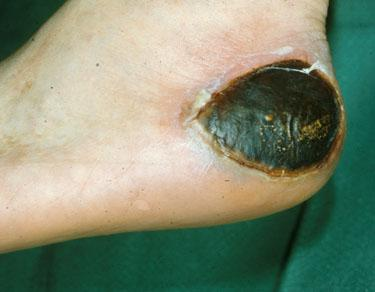
\includegraphics[width=\textwidth]{gambar/gambar-3_2(b).jpg}
		\caption{}
	  \end{subfigure}  
	  \begin{subfigure}{0.2\textwidth}
		\centering{}
		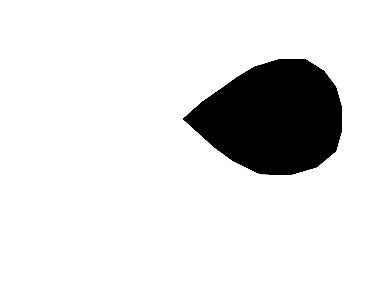
\includegraphics[width=\textwidth]{gambar/gambar-3_2(c).jpg}
		\caption{}
	  \end{subfigure}
	  \begin{subfigure}{0.2\textwidth}
		\centering{}
		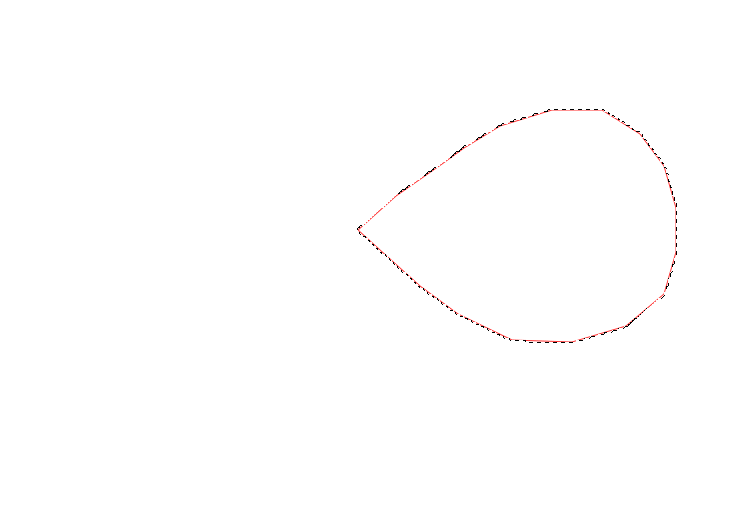
\includegraphics[width=\textwidth]{gambar/gambar-3_2(d).png}
		\caption{}
	  \end{subfigure}  
	\caption{
		(a)Data citra format .xcf, (b) \emph{layer} citra (luka), (c) \emph{layer} 
		region, (d)path
	 }
    \label{img:dataset_persiapan}
  \end{figure}

Langkah selanjutnya adalah peneliti memasukkan data citra \ref{img:dataset_persiapan}(b) ke dalam figma untuk
membuat \emph{layer} dan region (luka) dengan menggunakan \emph{pen tools}, hasil 
dari \emph{pen tools} akan berupa \emph{stroke} atau seperti path \ref{img:dataset_persiapan}(d), kemudian 
peneliti menduplikasi hasil path dan mengubahnya menjadi objek (\emph{fill object})
seperti \ref{img:dataset_persiapan}(c).

\begin{figure}[H]
	\centering{}
	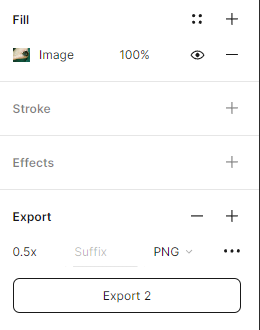
\includegraphics[width=0.3\textwidth]{gambar/gambar-3_4.png}
	\caption{Proses \emph{resize} citra gambar luka dengan ukuran 0.5 dari ukuran awal}
  \end{figure}

Setelah peneliti melakukan \emph{resize} ukuran citra, selanjutnya peneliti \emph{export}
\emph{layer} masing masing ke format .jpg.

% \begin{figure}[H]
% 	\centering{}
% 	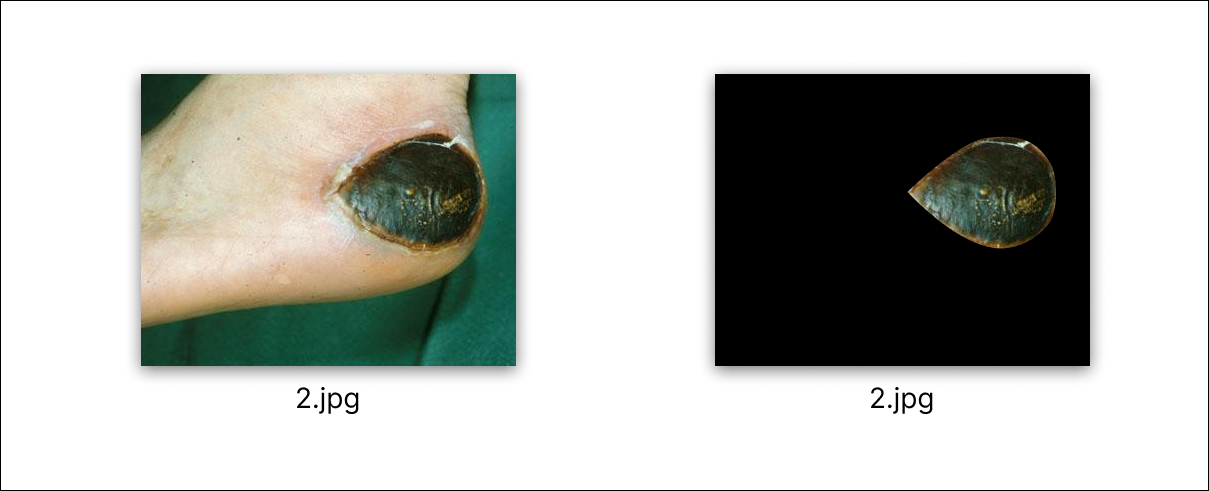
\includegraphics[width=\textwidth]{gambar/gambar-3_5.png}
% 	\caption{Citra gambar luka dan \emph{region} luka}
% \end{figure}

\subsection{Inisiai \emph{Bounding Box} di area luka}

Peneliti memulai dengan menentukan kotak pembatas (\emph{bounding box}) yang mengelilingi 
objek yang ingin dipisahkan. Area di dalam \emph{bounding box} akan digunakan untuk membuat 
\emph{Trimap Unknown} \((T_{U})\), sementara area di luar \emph{bounding box} dianggap sebagai Trimap 
Background \((T_{B})\). Setiap piksel yang termasuk dalam \((T_{B})\) akan memiliki nilai 
\(\alpha_{n}\) sama dengan 0, sedangkan piksel yang termasuk dalam \((T_{U})\) akan memiliki nilai 
\(\alpha_{n}\) sama dengan 1. \emph{Bounding box} digunakan untuk mempercepat waktu komputasi algoritma dan meningkatkan 
akurasi segmentasi.

\begin{figure}[H]
	\centering{}
    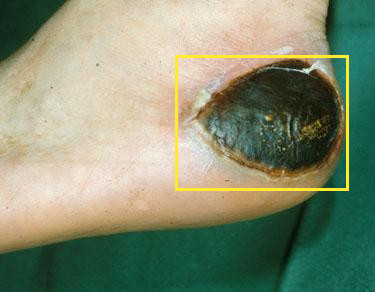
\includegraphics[width=0.3\textwidth]{gambar/rectangle.png}
	\caption{Inisiasi area objek luka dengan \emph{bounding box}}
\end{figure}

\subsection{Inisiasi GMM}

Pertama peneliti akan melakukan inisiasi untuk tiap parameter GMM, di antaranya 
\(\{\mu, \Sigma \}\), pada algoritma \emph{grabcut} akan digunakan K = 5. Adapun
inisiasi yang dilakukan adalah membuat nilai random terhadap \(\mu\) dan \(\Sigma\).
setelah itu peneliti menentukan \(\omega_k = \frac{1}{5}\), untuk \(k \in \{1, ..., 5\}\).
Distribusi gaussian yang akan digunakan untuk citra gambar berwarna yaitu distribusi 
gaussian \emph{multivariate} 2 dimensi atau 3 dimensi.
% sebagai ilustrasi gausian berdistribusi 
% normal 2 dimensi dengan objek citra gambar luka berwarna.

% \begin{figure}[H]
% 	\centering
% 	\begin{subfigure}{0.3\textwidth}
% 		\centering{}
% 		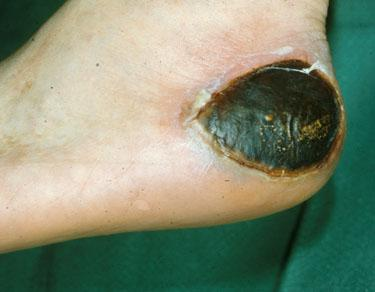
\includegraphics[width=\textwidth]{gambar/gambar-3_2(b).jpg}
% 		\caption{}
% 	\end{subfigure}
%     % \hfill% or \hspace{5mm} or \hspace{0.3\textwidth}
% 	\begin{subfigure}{0.3\textwidth}
% 		\centering{}
% 		\includegraphics[width=\textwidth]{gambar/gambar-3_7.png}
% 		\caption{}
% 	\end{subfigure} 
% 	\caption{
% 		(a) Citra gambar luka, (b) Deteksi \emph{clustering} citra dengan GMM
% 	}
%     \label{img:ilustrasi_gmm_2dimensi}
% \end{figure}

\subsection{Mempelajari parameter GMM}

Tahapan mempelajari parameter GMM dalam algoritma \emph{GrabCut} adalah untuk 
menghasilkan model yang akurat dalam memodelkan distribusi warna dari objek 
dan latar belakang dalam gambar. Tahap ini digunakan untuk memperbarui parameter-parameter 
GMM berdasarkan probabilitas posteriori. Algoritma menggunakan probabilitas posteriori 
piksel sebagai bobot dalam perhitungan rata-rata dan kovariansi baru untuk setiap 
komponen GMM. Dengan demikian, piksel yang memiliki probabilitas posteriori yang 
lebih tinggi akan memberikan kontribusi yang lebih besar dalam perhitungan parameter GMM.

Langkah dalam memperbarui parameter GMM dilakukan dengan langkah-langkah sebagai berikut:
\begin{enumerate}
    \item Untuk setiap komponen GMM dalam model objek dan latar belakang, hitung 
    rata-rata baru. Rata-rata baru dihitung dengan menggunakan probabilitas posteriori 
    piksel sebagai bobot dalam perhitungan rata-rata.
    \item Selanjutnya, perbarui kovariansi baru untuk setiap komponen GMM. Perhitungan 
    kovariansi baru juga menggunakan probabilitas posteriori sebagai bobot dalam 
    perhitungan kovariansi.
    \item Setelah perhitungan rata-rata dan kovariansi baru selesai untuk semua 
    komponen GMM, model GMM telah diperbarui.
\end{enumerate}

Dengan memperbarui parameter-parameter GMM berdasarkan probabilitas posteriori yang 
dihitung, algoritma secara bertahap meningkatkan model GMM agar sesuai dengan data gambar. 
Model yang lebih akurat membantu algoritma dalam membedakan antara piksel objek dan 
latar belakang, sehingga memperbaiki hasil segmentasi dengan lebih baik.


\subsection{Segmentasi Citra dengan Algoritma \emph{Mincut}}

Selanjutnya peneliti melakukan segmentasi dengan menggunakan algoritma \emph{min-cut}
atau \emph{GraphCut}. Algoritma ini memvisualisasikan gambar sebagai graf, dan piksel 
sebagai \emph{node} pada graf tersebut, kemudian \emph{GraphCut} bertugas untuk 
segmentasi piksel mana yang termasuk \emph{foreground} dan \emph{background} dengan cara
melakukan \emph{cut} pada graf. 

% Terdapat dua terminal pada graf yaitu terminal \emph{source} s
% dan \emph{sink} t, kedua terminal saling terhubung terhadap semua piksel yang ada di graf,
% piksel yang masuk ke dalam \emph{source} akan menjadi \emph{foreground} sementara piksel
% yang masuk ke dalam \emph{sink} akan menjadi \emph{background}. Setiap \emph{node} 
% pada graf memiliki hubungan yang yang disebut \emph{edge}, \emph{edge} akan memiliki arah 
% dan bobot dimana bobot tersebut akan digunakan untuk mencari \emph{mincut} dari graf.


\begin{figure}[H]
	\centering
	  \begin{subfigure}{.5\textwidth}
		\centering{}
		\includegraphics[width=\textwidth]{gambar/cth-graph-1.png}
		\caption{Sebuah graf}
	  \end{subfigure} \hfill
	  \begin{subfigure}{.5\textwidth}
		\centering{}
		\includegraphics[width=\textwidth]{gambar/cth-graph-2.png}
		\caption{Sebuah (\emph{cut})}
	  \end{subfigure}  
	\caption{
	  Contoh graf berkapasitas terarah.
	  }
	\label{img:contoh_mincut}
  
  \end{figure}

% Algoritma \emph{mincut} terdiri dari beberapa tahap, penjelasan singkatnya yaitu 
% tahap pertama dimana graf bertumbuh (\emph{growth}) hingga menemukan jalan (\emph{path}) 
% dari \emph{source} menuju \emph{sink}, selanjutnya tahap kedua (augmentasi) dimana 
% \emph{path} yang sudah ditemukan akan dilihat kapasitas tiap \emph{edge} nya lalu 
% masing-masing kapasitas \emph{edge} akan dikurangi dengan kapasitas paling kecil 
% (\emph{bottleneck}), apabila ada kapasitas \emph{edge} yang kosong, maka \emph{node} 
% tersebut menjadi \emph{Orphans} (tidak memiliki orang tua), setelah itu masuk tahap 
% ketiga (adopsi) yaitu mencari orang tua baru dari \emph{node} yang menjadi \emph{orphans} 
% sebelumnya, apabila tidak ada maka \emph{node} tersebut menjadi \emph{node} bebas. 
% Struktur algoritma \emph{mincut} dapat dilihat pada bagian \ref{pseudo:1.0}. 

Setiap piksel pada gambar memiliki komponen GMM tersendiri, pada tahap ini nilai k
tiap piksel telah didapatkan dari GMM, dimana nilai k dari tiap piksel memiliki rentang
dari 1 sampai 5. Pada permulaan algoritma \emph{mincut} peneliti menentukan \emph{node}
mana yang menjadi tetangga dari \emph{source} atau \emph{sink} dengan menghitung
jumlah nilai D dari persamaan \ref{eq:rumus_energi2} pada setiap komponen GMM, 
kemudian peneliti menjumlahkan nilai yang didapat dan membaginya dengan 5 (total K),
nilai yang didapat akan dijadikan sebagai \emph{treshold} dalam menentukan hubungan
tiap piksel ke \emph{Source} atau ke \emph{Sink}. Tahap ini mensegmentasi citra 
yang telah dihitung setiap komponen pikselnya pada langkah-langkah sebelumnya sesuai 
dengan persamaan \ref{eq:rumus_energi1}.

% \begin{lstlisting} [label={pseudo: neighbors_terminals}]
% 	initialize: (P = [[], [], [], [], []], 
% 	S = [0,0,0,0,0], 
% 	G = (V, E), K = Himpunan komponen GMM tiap piksel)
% 	t = 0
% 	for every node x $\in$ V : 
% 		P[K[x]-1] := P[K[x]-1] $\cup$ {x}
% 		Calculate D for x using $\ref{eq:2.12}$
% 		S[K[x]-1] += D
% 	end for

% 	Calculate t := mean(S)  7425, 7522, 98,694

% 	for every k $\in$ {1,2,3,4,5}:
% 	if S[k-1] < t
% 		E := E $\cup$ (s $\rightarrow$ p) for every p $\in$ P[k-1]
% 	else
% 		E := E $\cup$ (p $\rightarrow$ t) for every p $\in$ P[k-1]
% 	end for

	
%   \end{lstlisting}

% Selanjutnya masuk ke tahap growth, \emph{augmentation}, dan \emph{adoption}, diagram alir
% dari ketiga tahap bisa dilihat sebagai berikut :

% dengan meminimumkan rumus E pada persamaan \ref{eq:2.10}, lalu kembali
% ke langkah awal sampai terjadinya konvergensi yaitu tidak ada perbedaan segmentasi antar Iterasi.

% \subsection{Penyuntingan oleh Pengguna}
% Langkah selanjutnya peneliti melakukan perbaikan dari citra yang telah tersegmentasi
% dari hasil sebelumnya, pengguna menggunakan \emph{brush} yaitu menggambar manual daerah 
% yang menjadi \emph{background} dengan warna hitam, dan daerah objek dengan warna putih
% kemudian melakukan algoritma \emph{mincut} yang hanya dilakukan sekali. Berikut 
% gambaran simulasi penelitian yang akan peneliti lakukan terhadap citra gambar luka 
% untuk mendapatkan hasil segmentasi dengan metode \emph{GrabCut}:

\begin{figure}[H]
	\centering
	  \begin{subfigure}{0.3\textwidth}
		\centering{}
		\includegraphics[width=\textwidth]{gambar/gambar-3_2(b).jpg}
		\caption{}
	  \end{subfigure}  
	  \begin{subfigure}{0.3\textwidth}
		\centering{}
		\includegraphics[width=\textwidth]{gambar/rectangle.png}
		\caption{}
	  \end{subfigure}
      \begin{subfigure}{0.3\textwidth}
		\centering{}
		\includegraphics[width=\textwidth]{gambar/res_2.png}
		\caption{}
	  \end{subfigure}
	\caption{
		(a) Data citra luka 2.png, (b) \emph{Bounding box} area luka, (c) Hasil segmentasi citra
	 }
  \end{figure}

\subsection{Menghitung Tingkat Akurasi}
Untuk menemukan nilai hasil segmentasi citra luka dengan menggunakan algoritma \emph{GrabCut},
yaitu mencari nilai akurasi citra, dengan menghitung selisih piksel dari area
segmentasi dengan area citra referensi sehingga akan menghasilkan nilai akurasi berikut :
\begin{equation} \label{eq:validasi}
	Akurasi(\%) = 100 - \bigg | \frac{(luas \: area \: citra \: referensi - luas \: area \: segmentasi)}{luas \: area \: citra \: referensi} * 100 \bigg |
\end{equation}.


\section{Skenario Eksperimen} \label{section:skenario_eksperimen}

Berikut adalah skenario eksperimen untuk "Deteksi Area Keliling Luka Kronis 
Menggunakan \emph{GRABCUT}"

\begin{enumerate}
    \item{Input gambar luka kronis}
    \item{Pengguna memberi kotak pembatas di sekeliling area luka (objek) pada gambar luka}
    \item{Inisiasi titik koordinat \((x,y)\) kotak pembatas di dalam gambar luka}
    \item{Memberi penanda area di luar kotak dengan angka 1, dan area di luar kotak
    dengan angka 0}
    \item{Memasukkan komponen GMM di setiap piksel untuk menghitung probabilitas 
    tiap piksel }
    \item{Mempelajari parameter GMM dengan melihat hasil probabilitas objek atau latar belakang}
    \item{Segmentasi area keliling luka dengan menggunakan algoritma \emph{GraphCut}}
    \item{Ulangi sampai sesuai dengan area luka}
    \item{Mendapatkan nilai akurasi}
  \end{enumerate}
%!TEX root = ./template-skripsi.tex
%-------------------------------------------------------------------------------
%                            	BAB IV
%               		KESIMPULAN DAN SARAN
%-------------------------------------------------------------------------------

\chapter{HASIL DAN PEMBAHASAN}

\section{Pemrosesan citra gambar input}
Langkah pertama dalam pemrosesan citra gambar input adalah menentukan rasio piksel 
dari citra tersebut, peneliti mengubah lebar citra menjadi 320 piksel untuk efisiensi 
serta menyamakan ukuran tiap sampel citra gambar, berikut \emph{source code} nya:

\begin{figure}[H]
	\begin{lstlisting}[language=Python, basicstyle=\tiny]
		def setSizeImg(self):
			global new_width, aspect_ratio, new_height
			# set ukuran gambar
			new_width = 320  # Atur ukuran hanya 320 px
			aspect_ratio = self.image.width / self.image.height
			new_height = int(new_width / aspect_ratio)
		
		# Laod image
		self.image = Image.open(self.image_path)

		# Resize ukuran gambar
		self.setSizeImg() 
		self.image = self.image.resize((new_width, new_height)) 
	\end{lstlisting}
	\caption{\emph{source code} mengubah ukuran lebar citra menjadi 320 piksel}
	\label{code:resize_gambar}
\end{figure}

Fungsi \texttt{setSizeImg()} dibuat untuk mengubah ukuran lebar piksel citra 
menjadi 320 piksel, untuk mempertahankan rasionya, maka dibentuk dengan menghitung
menggunakan rumus \texttt{aspect\_ratio} dimana tinggi gambar akan otomatis mengikuti lebar gambar 
dengan perbandingan yang tetap.

\section{Deteksi keliling luka menggunakan \emph{Grabcut}}
Alur deteksi keliling luka menggunakan algoritma \emph{Grabcut} dilakukan melalui
beberapa tahapan, setiap tahapan akan mengolah data input berupa citra gambar luka 
yang disimpan menjadi \emph{array} multidimensi (lebar, tinggi, nilai RGB).
Berikut adalah tahapannya:

\subsection{Inisiasi Kotak Pembatas (\emph{Bounding Box})}

Dalam segmentasi citra luka, dimulai dengan inisiasi kotak atau \emph{bounding box} 
yang digambar mengelilingi area citra luka, berikut \emph{source code} nya:
\begin{figure}[H]
	\begin{lstlisting}[language=Python, basicstyle=\tiny]
		def drawing_rectangle(self):
			print("mulai gambar kotak")
			self.main_canvas.bind("<ButtonPress-1>", self.onClick_rect)
			self.main_canvas.bind("<B1-Motion>", self.onDrag_rect)
			self.main_canvas.bind("<ButtonRelease-1>", self.onRelease_rect)

		def onClick_rect(self, event):
			print("Keberadaan kotak: ",KOTAK["is_drawn"])
			if KOTAK["is_drawn"] is not True:
				KOTAK["titik_start"] = (event.x, event.y)
			else:
				print("kotak sudah ada")

		def onDrag_rect(self, event):
			if KOTAK["is_drawn"] is not True:
				KOTAK["titik_akhir"] = (event.x, event.y)
				self.update_image()

		def onRelease_rect(self, event):
			if KOTAK["titik_start"] and KOTAK["titik_akhir"]:
				KOTAK["coord"] = (self.get_rectangle_coords())
				print("Koordinat Kotak: ", KOTAK["coord"])
				KOTAK["titik_start"] = None
				KOTAK["titik_akhir"] = None
				KOTAK["is_drawn"] = True
			print("Keberadaan kotak: ",KOTAK["is_drawn"])
			print("Koordinat Kotak: ", KOTAK["coord"])

		def get_rectangle_coords(self):
			if KOTAK["titik_start"] and KOTAK["titik_akhir"]:
				x1, y1 = KOTAK["titik_start"]
				x2, y2 = KOTAK["titik_akhir"]
				return (x1, y1, x2, y2)
			else:
				return None

		def drawing_rectangle(self):
			print("mulai gambar kotak")
			self.main_canvas.bind("<ButtonPress-1>", self.onClick_rect)
			self.main_canvas.bind("<B1-Motion>", self.onDrag_rect)
			self.main_canvas.bind("<ButtonRelease-1>", self.onRelease_rect)

	\end{lstlisting}
	\caption{\emph{source code} menggambar kotak pada area luka}
	\label{code:inisiasi_rectangle}
\end{figure}

Ketika kotak sudah tergambar, koordinat dimasukkan kedalam variabel \texttt{KOTAK["coord"]}
pada fungsi \texttt{onRelease\_rect()} yang mana \texttt{KOTAK["coord"]} berupa array 
berisi x1, y1, x2, y2 yang akan digunakan untuk tahap selanjutnya.

\subsection{Inisiasi Piksel}
Tahap selanjutnya adalah membuat salinan \emph{masking} pada citra gambar luka yang diubah
menjadi gambar hitam, salinan dibuat dengan menggunakan \emph{library} \emph{Numpy}
dengan target citra gambar luka. Berikut \emph{source code} nya:

\begin{figure}[H]
	\begin{lstlisting}[language=Python, basicstyle=\tiny]
	self.gambar = np.array(self.image)
	self.gambar2 = self.gambar.copy()
	self.mask = np.zeros(self.gambar2.shape[:2], dtype=np.uint8)
	self.mask2 = self.mask.copy()

	def inisiasi_piksel(self):
		self.alpha[self.rect[1]:self.rect[1] + self.rect[3],self.rect[0]:self.rect[0] + self.rect[2]] = F_TF
		self.trimap['TB'] = np.where(self.alpha == F_TB)
		self.trimap['TU'] = np.where(self.alpha == F_TF)
		"""Inisiasi GMM"""
		self.gmm_fg =  MixtureModel(self.trimap['TU'], 
						self.gambar[self.trimap['TU']], 
						self.komponen_gmm, self.theta['TU'])
		self.gmm_bg =  MixtureModel(self.trimap['TB'], 
						self.gambar[self.trimap['TB']], 
						self.komponen_gmm, self.theta['TB'])
		self.gmm_fg.init_gmm_rand(self.gambar[self.trimap['TU']], self.theta['TU'])
		self.gmm_bg.init_gmm_rand(self.gambar[self.trimap['TB']], self.theta['TB'])
	\end{lstlisting}
	\caption{\emph{source code} inisasi objek gmm \emph{foreground} dan \emph{background} }
	\label{code:mask_image}
\end{figure}

Variabel  \texttt{self.gmm\_fg} dan \texttt{self.gmm\_bg} dibuat sebagai penanda antara objek untuk
\emph{foreground} dan \emph{background}, masing masing memiliki parameter \texttt{self.gambar}, 
\texttt{self.theta}, \texttt{self.trimap}, dan \texttt{self.komponen\_gmm}. Parameter 
tersebut dibedakan nilainya yakni \textbf{'TU'} atau \textbf{'TB'}. 

\begin{figure}[H]
	\begin{lstlisting}[language=Python, basicstyle=\tiny]
	def init_gmm_rand(self, z, theta):
        labels_k = []
        for i in range(z.shape[0]):
            labels_k.append(random.randint(0, self.komponen_gmm-1))
        labels_k = np.array(labels_k)
        self.count_params(z, labels_k, theta)
	\end{lstlisting}
	\caption{\emph{source code} menentukan label awal secara acak}
	\label{code:init_gmm_random}
\end{figure}

Fungsi \texttt{init\_gmm\_rand()} memiliki tugas sebagai pembuat label gmm secara 
acak sepanjang  \texttt{self.gambar} dengan batas angka yakni dari angka 0 sampai 
\texttt{self.komponen\_gmm}, setelah label terbentuk dilanjutkan dengan menjalankan 
fungsi \texttt{count\_params} untuk menghitung nilai GMM berdasarkan nilai awal 
(inisiasi). Berikut \emph{source code} nya:

\subsection{Menentukan Komponen Awal GMM}
Tahap ini merupakan tahap pertama pada gambar \ref{img:segmentasi_grabcut}. Setelah
membuat variabel gmm (fg dan bg) didalamnya terdapat fungsi untuk menentukan dan 
menghitung komponen gmm awal. Berikut \emph{source code} nya:

\begin{figure}[H]
	\begin{lstlisting}[language=Python, basicstyle=\tiny]
	def assign_gmm(self):
        """Step 1 (assign GMM) pada gambar 2.11"""
        print('\nMulai assign GMM')
        self.komponen_piksel[self.trimap['TU']] = self.gmm_fg.assign_component(
            self.gambar[self.trimap['TU']], self.theta['TU'], self.komponen_gmm
        )
        self.komponen_piksel[self.trimap['TB']] = self.gmm_bg.assign_component(
            self.gambar[self.trimap['TB']], self.theta['TB'], self.komponen_gmm
        )
	\end{lstlisting}
	\caption{\emph{source code} menghitung nilai gmm menggunakan label awal}
	\label{code:assign_gmm}
\end{figure}

Fungsi \texttt{assign\_component} adalah fungsi yang menghitung nilai akumulasi 
dari distribusi probabilitas gaussian yang terdapat pada gambar \ref{img:segmentasi_grabcut}
tahap pertama. Berikut \emph{source code} nya:

\begin{figure}[H]
	\begin{lstlisting}[language=Python, basicstyle=\tiny]
	def assign_component(self, z, theta, komponen_gmm):
        gauss_distribution = []
        for k in range(komponen_gmm):
            gauss_score = self.dis_mult(z, k, theta)
            gauss_distribution.append(gauss_score)
        gauss_distribution = np.array(gauss_distribution)
        gauss_distribution = gauss_distribution.T

        return np.argmin(gauss_distribution, axis=1)
	\end{lstlisting}
	\caption{\emph{source code} menghitung akumulasi distribusi gaussian}
	\label{code:assign_component}
\end{figure}

Hasil dari tahap ini adalah label gmm yang telah dihitung yang kemudian akan dipakai 
di tahap selanjutnya.


\subsection{Mempelajari Parameter GMM}
Masuk ke tahap selanjutnya (kedua) dari gambar \ref{img:segmentasi_grabcut} dimana 
label gmm yang sudah diperbarui akan digunakan untuk menghitung kembali parameter 
gmm yakni \texttt{self.theta}. Berikut \emph{source code} nya:

\begin{figure}[H]
	\begin{lstlisting}[language=Python, basicstyle=\tiny]
	def mempelajari_gmm(self):
        self.gmm_fg.count_params(self.gambar[self.trimap['TU']], 
                                 self.komponen_piksel[self.trimap['TU']], 
                                 self.theta['TU'])

        self.gmm_bg.count_params(self.gambar[self.trimap['TB']], 
                                 self.komponen_piksel[self.trimap['TB']], 
                                 self.theta['TB'])

        idx_TU = np.where(self.alpha.reshape(-1) == F_TF)

		self.D_count_fg = []
        self.D_count_bg = []
        for kn in range(self.komponen_gmm):
            zn = self.gambar.reshape(-1, 3)[idx_TU]

            tmp_d_fg = self.gmm_fg.d_calc(zn, kn, self.theta['TU'])
            tmp_d_bg = self.gmm_bg.d_calc(zn, kn, self.theta['TB'])

            self.D_count_fg.append(tmp_d_fg)
            self.D_count_bg.append(tmp_d_bg)

        self.D_count_fg = np.array(self.D_count_fg)
        self.D_count_bg = np.array(self.D_count_bg)
        self.U_count_fg = np.sum(self.D_count_fg, axis=0)
        self.U_count_bg = np.sum(self.D_count_bg, axis=0)       
	\end{lstlisting}
	\caption{\emph{source code} mempelajari parameter GMM}
	\label{code:learn_gmm}
\end{figure}

Setelah mendapat parameter gmm yang baru, selanjutnya adalah menghitung nilai \(D\)
dengan menggunakan rumus \ref{eq:rumus_D}, fungsi yang menghitungnya terdapat pada 
fungsi \texttt{d\_calc}. Berikut \emph{source code} nya:

\begin{figure}[H]
	\begin{lstlisting}[language=Python, basicstyle=\tiny]
	def d_calc(self, zn, kn, theta):
        gauss_res1 = self.gauss_dist_second(zn, kn, theta)
        d_res1 = -np.log(theta['koefisien'][kn]) + gauss_res1

        return d_res1
	\end{lstlisting}
	\caption{\emph{source code} menghitung nilai D}
	\label{code:count_d}
\end{figure}

\subsection{Segmentasi Gambar dengan Algoritma \emph{Mincut}}
Tahap terakhir adalah segmentasi gambar dengan algoritma \emph{mincut}, tahap 
ini bertujuan untuk melakukan pemotongan gambar yang telah dikalkulasi pada 
tahap sebelumnya, algoritma ini membutuhkan adanya graf yang dibuat dari gambar 
citra, \emph{node} pada graf merepresentasikan piksel dalam citra. 
Berikut \emph{source code} nya:

\begin{figure}[H]
	\begin{lstlisting}[language=Python, basicstyle=\tiny]
	def build_graph(self):
		self.gc_graph = ig.Graph(self.kolom * self.baris + 1)
		self.gc_graph.add_edges(self.edges)
	\end{lstlisting}
	\caption{\emph{source code} Membangun graf}
	\label{code:build_graph}
\end{figure}

Setelah graf terbentuk, segmentasi akan dilakukan dengan algoritma \emph{mincut}.
Berikut \emph{source code} nya:
\begin{figure}[H]
	\begin{lstlisting}[language=Python, basicstyle=\tiny]
	def mincut_segmentation(self):

        mincut = self.gc_graph.st_mincut(
        self.source_gc, self.sink_gc, self.kapasitas_graph)

        idx_pr = np.where(self.alpha == F_TF)
        img_indexes = np.arange(self.baris * self.kolom,
                                dtype=np.uint32).reshape(self.baris, self.kolom)

        self.alpha[idx_pr] = np.where(np.isin(img_indexes[idx_pr], mincut.partition[0]),F_TF, F_TB)
	\end{lstlisting}
	\caption{\emph{source code} Membangun graf}
	\label{code:mincut_segmentation}
\end{figure}



\section{Eksperimen}
\emph{Source code} program disimpan di dalam repositori yang dapat diakses di
\url{https://github.com/DragonFly378/Skripsi_Hafiz} di bawah lisensi \emph{GNU General Public License v3.0.}
Rancangan eksperimen deteksi keliling luka dengan algoritma \emph{Grabcut}. Proses 
ini diperlukan adanya penyesuaian parameter dari algoritma yang dijalankan dengan 
data yang tersedia untuk setiap citra. Setelah hasil segmentasi citra didapatkan,
dilanjutkan dengan identifikasi citra hasil segmentasi dan dibandingkan terhadap area 
\emph{ground truth} untuk kemudian dihitung akurasinya menggunakan persamaan \ref{eq:validasi}.
Rincian lengkap hasil dari parameter dan validasi citra tersedia di bagian \textbf{lampiran C}.

\begin{figure}[H]
	\centering
	\includegraphics[width=0.8\textwidth]{gambar/hasil_bab4.jpg}
	\caption{(a) Kotak pembatas (b) Hasil segmentasi (c) Area \emph{ground truth} (d) Akurasi}
	\label{img:hasil_segmentasi}
\end{figure}

\section{Analisa hasil}
Berikut analisa hasil setelah melakukan eksperimen terhadap populasi:
\begin{enumerate}
	\item Hasil dari deteksi keliling luka menggunakan \emph{snake} versi \emph{integer} kategori luka hitam menghasilkan 5 data (dari 24 data) yang kurva akhirnya berhasil menutupi luka dengan nilai akurasi rata-rata 84.2\%.
	\item Hasil dari deteksi keliling luka menggunakan \emph{snake} versi \emph{integer} kategori luka kuning menghasilkan 5 data (dari 15 data) yang kurva akhirnya berhasil menutupi luka dengan nilai akurasi rata-rata 76.14\%.
	\item Hasil dari deteksi keliling luka menggunakan \emph{snake} versi \emph{integer} kategori luka merah menghasilkan 2 data (dari 30 data) yang kurva akhirnya berhasil menutupi luka dengan nilai akurasi rata-rata 62.25\%.
	\item Hasil dari deteksi keliling luka menggunakan \emph{snake} versi \emph{intepolasi} kategori luka hitam menghasilkan 21 data (dari 24 data) yang kurva akhirnya berhasil menutupi luka dengan nilai akurasi rata-rata 87.6\%.
	\item Hasil dari deteksi keliling luka menggunakan \emph{snake} versi \emph{interpolasi} kategori luka kuning menghasilkan 11 data (dari 15 data) yang kurva akhirnya berhasil menutupi luka dengan nilai akurasi rata-rata 79.2\%.
	\item Hasil dari deteksi keliling luka menggunakan \emph{snake} versi \emph{interpolasi} kategori luka merah menghasilkan 12 data (dari 30 data) yang kurva akhirnya berhasil menutupi luka dengan nilai akurasi rata-rata 89.7\%.
	\item Hasil dari deteksi keliling luka menggunakan \emph{snake} versi \emph{integer} untuk semua kategori menghasilkan 12 data (dari 71 data) yang kurva akhirnya berhasil menutupi luka dengan nilai akurasi rata-rata 77.18\%.
	\item Hasil dari deteksi keliling luka menggunakan \emph{snake} versi \emph{integer} untuk semua kategori menghasilkan 44 data (dari 71 data) yang kurva akhirnya berhasil menutupi luka dengan nilai akurasi rata-rata 86.1\%.
\end{enumerate}

% Baris ini digunakan untuk membantu dalam melakukan sitasi
% Karena diapit dengan comment, maka baris ini akan diabaikan
% oleh compiler LaTeX.
\begin{comment}
\bibliography{daftar-pustaka}
\end{comment}
%!TEX root = ./template-skripsi.tex
%-------------------------------------------------------------------------------
%                            	BAB IV
%               		KESIMPULAN DAN SARAN
%-------------------------------------------------------------------------------

\chapter{KESIMPULAN DAN SARAN}

\section{Kesimpulan}
Berdasarkan hasil implementasi dan pengujian fitur sistem informasi yang telah dirancang, maka diperoleh kesimpulan sebagai berikut:

\begin{enumerate}
	\item Perancangan sistem informasi operasi serba usaha berbasis \emph{website} pada lembaga Koperasi Mahasiswa Universitas Negeri Jakarta menggunakan metode pengembangan perangkat lunak \textit{System Development Life Cycle} dengan \textit{spiral model} yang memiliki beberapa tahapan, yaitu analisis kebutuhan, perancangan desain sistem \textit{(prototype)}, pengimplementasian (\textit{coding \& testing-unit}), dan \textit{maintenance} (umpan balik dan tanggapan).
	
	\item Sistem informasi Koperasi Mahasiswa Universitas Negeri Jakarta dibangun dengan menggunakan \textit{framework codeigniter} dan \textit{framework bootstrap}. \textit{Codeigniter} untuk membangun sisi dalam \textit{back-end} dan \textit{Bootstrap} yang mempercantik bagian luar \textit{front-end}. Berdasarkan pengolahan data hasil kuesioner \textit{user acceptance test}, didapatkan rata-rata persentase mencapai angka 4,27 dari 5 atau sekitar 85\% untuk \textit{admin} yang berarti sistem sudah sangat sesuai, 3,96 dari 5 atau sekitar 79\% untuk anggota yang berarti sistem sudah sesuai, dan 4,53 dari 5 atau sekitar 91\% pada sistem pengawas yang berarti sistem sudah sangat sesuai.
	
	\item Sistem informasi Koperasi Mahasiswa Universitas Negeri Jakarta berbasis \textit{website} dibangun agar sistem pengelolaan data di KOPMA UNJ dapat menjadi lebih efektif dan efisian, serta agar kemungkinan adanya \textit{human error} dapat di atasi. Data yang dikelola berupa data anggota, barang, stok (pergudangan), simpanan, transaksi, penilaian, dan keuangan.
	
	\item Sistem informasi Koperasi Mahasiswa Universitas Negeri Jakarta berbasis \textit{website} mempermudah \textit{admin} dalam melakukan pengelolaan data yang ada di KOPMA UNJ, mempermudah pengawas dalam melakukan pengelolaan data penilan, dan membuat anggota dapat mengetahui transparansi simpanan yang mereka bayarkan hingga mengetahui transparansi sisa hasil usaha yang mereka dapatkan.
\end{enumerate}

\section{Saran}
Adapun saran untuk penelitian selanjutnya adalah:
\begin{enumerate} 
	\item Mengintegrasikan sistem informasi KOPMA UNJ dengan aplikasi dan sistem \textit{scanning barcode} agar proses transaksi semakin efektif dan efisien.
	\item Menambahkan dan mengintegrasikan sistem informasi KOPMA UNJ dengan aplikasi untuk \textit{scanning barcode} pada kartu anggota agar proses kebutuhan simpanan dan transaksi untuk anggota dapat semakin efektif dan efisien.
	\item Menambahkan sistem pengelolaan kegiatan keorganisasian KOPMA UNJ yang merupakan bagian dari peran KOPMA UNJ sebagai Organisasi Kemahasiswaan di UNJ.
	\item Membuat pengembangan sistem informasi KOPMA UNJ berbasis \textit{mobile} (\textit{android}).
\end{enumerate}


% Baris ini digunakan untuk membantu dalam melakukan sitasi
% Karena diapit dengan comment, maka baris ini akan diabaikan
% oleh compiler LaTeX.
\begin{comment}
\bibliography{daftar-pustaka}
\end{comment}

%-----------------------------------------------------------------
%Disini akhir masukan Bab
%-----------------------------------------------------------------


%-----------------------------------------------------------------
% Disini awal masukan untuk Daftar Pustaka
% - Daftar pustaka diambil dari file .bib yang ada pada folder ini
%   juga.
% - Untuk memudahkan dalam memanajemen dan menggenerate file .bib
%   gunakan reference manager seperti Mendeley, Zotero, EndNote,
%   dll.
%-----------------------------------------------------------------
% \bibliography{daftar-pustaka}
% \bibliographystyle{apalike}
\addcontentsline{toc}{chapter}{DAFTAR PUSTAKA}
\singlespacing{}
\printbibliography{}
%-----------------------------------------------------------------
%Disini akhir masukan Daftar Pustaka
%-----------------------------------------------------------------

\appendix


\chapter{\emph{Source code} program}

\section{main.py}
\begin{lstlisting}[language=Python,basicstyle=\tiny]
import sys
from image_editing import ImageEditing
from tkinter import *
from grabcut import GrabCut
from PIL import Image,ImageTk,ImageMath,ImageDraw
import numpy as np

if __name__ == '__main__':
    root = Tk()
    category = "luka_hitam"
    img_name = "2"
    extension = ".jpg"
    image_path = "dataset_3/"+category+"/"+img_name+extension
    tools = ImageEditing(root,image_path,img_name,category)
    root.mainloop()
\end{lstlisting}

\section{image\_editing.py}
\begin{lstlisting}[language=Python,basicstyle=\tiny]
import sys
import os
from tkinter import *
from grabcut import GrabCut
from PIL import Image,ImageTk,ImageMath,ImageDraw
import numpy as np

COLOR = {
    'red' : [0,0,255],
    'white' : [255,255,255],
    'black' : [0,0,0],
    'yellow' : "#FFFF00"
}

F_BG = 0
F_FG = 1
F_PR_FG = 2

KOTAK = {
    "coord" : (),
    "pos" : None,
    "titik_start" : None,
    "titik_akhir" : None,
    'is_init' : False,
    'is_drawn' : False,
}

BRUSH = {
    "size" : 3,
    'is_init' : False,
    'is_drawn' : False,
}

class ImageEditing:
    def __init__(self,root,image_path,image_name,category):
        self.root = root
        self.root.title("Image Segmentation using Grabcut")   
        self.image_path = image_path    
        self.image_name = image_name
        self.category = category

        # Create a frame for title labels
        self.title_frame = Frame(self.root)
        self.title_frame.pack(side=TOP,fill=X)

        # Create a frame for canvases
        self.canvas_frame = Frame(self.root)
        self.canvas_frame.pack(side=TOP,fill=BOTH,expand=YES)  # Adjusted to fill both X and Y,expand

        # Create a frame for buttons
        self.button_frame = Frame(self.root)
        self.button_frame.pack(side=BOTTOM,fill=BOTH)

        # Laod image
        self.image = Image.open(self.image_path)

        # Resize ukuran gambar
        self.setSizeImg() 
        self.image = self.image.resize((new_width,new_height)) # <-- untuk resize ukuran

        self.gambar = np.array(self.image)
        self.gambar2 = self.gambar.copy()
        print("ukuran gambar: ",self.gambar.shape)

        # buat masking dari gambar awal
        self.mask = np.zeros(self.gambar2.shape[:2],dtype=np.uint8)
        self.mask2 = self.mask.copy()

        self.LoadCanvas()

    def LoadCanvas(self):    
        # Make image as main canvas
        main_title_label = Label(self.title_frame,text="Main Canvas",font=('Helvetica',10,'bold'))
        self.photo = ImageTk.PhotoImage(self.image)
        self.main_canvas = Canvas(self.canvas_frame,width=self.image.width,height=self.image.height)
        self.main_canvas.create_image(0,0,anchor=NW,image=self.photo)

        # Create mask canvas
        mask_title_label = Label(self.title_frame,text="Mask Canvas",font=('Helvetica',10,'bold'))
        self.mask_image = Image.fromarray(self.mask)
        self.mask_image = self.mask_image.resize((new_width,new_height)) # <-- untuk resize ukuran
        self.mask_photo = ImageTk.PhotoImage(self.mask_image)
        self.mask_canvas = Canvas(self.canvas_frame,width=self.image.width,height=self.image.height)
        self.mask_canvas.create_image(0,0,anchor=NW,image=self.mask_photo)

        # Create a result canvas for result display
        result_title_label = Label(self.title_frame,text="Result Canvas",font=('Helvetica',10,'bold'))
        self.result_image = Image.new("RGB",(self.image.width,self.image.height))
        self.result_photo = ImageTk.PhotoImage(self.result_image)
        self.result_canvas = Canvas(self.canvas_frame,width=self.image.width,height=self.image.height)
        self.result_canvas.create_image(0,0,anchor=NW,image=self.result_photo)

        
        # Create the buttons with custom styles
        self.draw_rect_button = Button(self.button_frame,text="Draw Rectangle",command=self.drawing_rectangle,bg='#4CAF50',fg='white',font=('Helvetica',10))
        self.segmentation_button = Button(self.button_frame,text="Segmentation Grabcut",command=self.segmentation_image,bg='#2196F3',fg='white',font=('Helvetica',10))
        self.save_button = Button(self.button_frame,text="Save Result",command=self.save_result_image,bg='#FFC107',fg='black',font=('Helvetica',10))
        self.reset_button = Button(self.button_frame,text="Restart Program",command=self.reset_image,bg='#607D8B',fg='white',font=('Helvetica',10))
        
        # Display canvas
        self.main_canvas.pack(side=LEFT)
        main_title_label.pack(side=LEFT,padx=(10,220))
        self.mask_canvas.pack(side=LEFT)
        mask_title_label.pack(side=LEFT,padx=(10,220))
        self.result_canvas.pack(side=LEFT)
        result_title_label.pack(side=LEFT,padx=(10,220))

        # Display Buttons
        self.draw_rect_button.pack(side=LEFT,expand=YES,fill=BOTH,padx=5,pady=(10,10))
        self.segmentation_button.pack(side=LEFT,expand=YES,fill=BOTH,padx=5,pady=(10,10))
        self.save_button.pack(side=LEFT,expand=YES,fill=BOTH,padx=5,pady=(10,10))        
        self.reset_button.pack(side=LEFT,expand=YES,fill=BOTH,padx=5,pady=(10,10))

    def setSizeImg(self):
        global new_width,aspect_ratio,new_height
        # set ukuran gambar
        new_width = 320  # Atur ukuran hanya 480 px
        aspect_ratio = self.image.width / self.image.height
        new_height = int(new_width / aspect_ratio)

    def drawing_brush(self):
        print("mulai gambar brush")

    def drawing_rectangle(self):
        print("mulai gambar kotak")
        self.main_canvas.bind("<ButtonPress-1>",self.onClick_rect)
        self.main_canvas.bind("<B1-Motion>",self.onDrag_rect)
        self.main_canvas.bind("<ButtonRelease-1>",self.onRelease_rect)

    def onClick_rect(self,event):
        print("Keberadaan kotak: ",KOTAK["is_drawn"])
        if KOTAK["is_drawn"] is not True:
            KOTAK["titik_start"] = (event.x,event.y)
        else:
            print("kotak sudah ada")


    def onDrag_rect(self,event):
        if KOTAK["is_drawn"] is not True:
            KOTAK["titik_akhir"] = (event.x,event.y)
            self.update_image()

    def onRelease_rect(self,event):
        if KOTAK["titik_start"] and KOTAK["titik_akhir"]:
            KOTAK["coord"] = (self.get_rectangle_coords())
            print("Koordinat Kotak: ",KOTAK["coord"])
            KOTAK["titik_start"] = None
            KOTAK["titik_akhir"] = None
            KOTAK["is_drawn"] = True
        print("Keberadaan kotak: ",KOTAK["is_drawn"])
        print("Koordinat Kotak: ",KOTAK["coord"])


    def update_image(self):
        # Update the main canvas with image and annotations
        self.image = Image.open(self.image_path)
        self.image = self.image.resize((new_width,new_height))  # <-- untuk resize ukuran
        self.image2 = self.image.copy()
        self.draw = ImageDraw.Draw(self.image)
        for coords in KOTAK["coord"]:
            self.draw.rectangle(coords,outline="yellow",width=2)
        self.draw.rectangle(self.get_rectangle_coords(),outline="yellow",width=2)
        self.photo = ImageTk.PhotoImage(self.image)
        self.main_canvas.create_image(0,0,anchor=NW,image=self.photo)
    
    def update_result(self):

		# Update mask canvas with segmentation
        self.mask_image = Image.fromarray(self.mask)
        self.mask_image = self.mask_image.resize((new_width,new_height)) # <-- untuk resize ukuran
        self.mask_photo = ImageTk.PhotoImage(self.mask_image)
        self.mask_canvas.create_image(0,0,anchor=NW,image=self.mask_photo)

        # Update image with segmentation
        self.result_image = Image.composite(self.image2,Image.new("RGB",self.image.size,"black"),self.mask_image)
        self.result_photo = ImageTk.PhotoImage(self.result_image)
        self.result_canvas.create_image(0,0,anchor=NW,image=self.result_photo)
   

    def get_rectangle_coords(self):
        if KOTAK["titik_start"] and KOTAK["titik_akhir"]:
            x1,y1 = KOTAK["titik_start"]
            x2,y2 = KOTAK["titik_akhir"]
            return (x1,y1,x2,y2)
        else:
            return None

    def segmentation_image(self):
        gc = GrabCut(self.gambar2,self.mask2,KOTAK["coord"])
        self.mask = np.where((self.mask2 == F_FG) | (self.mask2 == F_PR_FG),255,0).astype('uint8')
        self.update_result()


    def save_result_image(self):
        save_folder = f"results/{self.category}"

        # Create the folder if it doesn't exist
        os.makedirs(save_folder,exist_ok=True)

        result_filename = f"result_{self.image_name}.jpg"
        main_rect_filename = f"image_{self.image_name}_rect.jpg"

        self.result_image.save(os.path.join(save_folder,result_filename))
        self.image.save(os.path.join(save_folder,main_rect_filename))

        print("Result image saved successfully:")

    def reset_image(self):
        # Reset image and mask to initial state
        self.image = Image.open(self.image_path)
        self.image = self.image.resize((new_width,new_height))  # <-- untuk resize ukuran
        self.gambar = np.array(self.image)
        self.gambar2 = self.gambar.copy()
        self.mask = np.zeros(self.gambar2.shape[:2],dtype=np.uint8)
        self.mask2 = self.mask.copy()

        # Reset annotation variables
        KOTAK["coord"] = ()
        KOTAK["is_init"] = False
        KOTAK["is_drawn"] = False

        # Reload main canvas
        self.photo = ImageTk.PhotoImage(self.image)
        self.main_canvas.create_image(0,0,anchor=NW,image=self.photo)

        # Clear the mask canvas
        self.mask_image = Image.fromarray(self.mask)
        self.mask_image = self.mask_image.resize((new_width,new_height)) # <-- untuk resize ukuran
        self.mask_photo = ImageTk.PhotoImage(self.mask_image)
        self.mask_canvas.create_image(0,0,anchor=NW,image=self.mask_photo)

        # Clear the result canvas
        self.result_image = Image.new("RGB",(self.image.width,self.image.height))
        self.result_photo = ImageTk.PhotoImage(self.result_image)
        self.result_canvas.create_image(0,0,anchor=NW,image=self.result_photo)

\end{lstlisting}

\section{grabcut.py}
\begin{lstlisting}[language=Python,basicstyle=\tiny]
import numpy as np 
from GMM import MixtureModel
import igraph as ig
from mincut import mincut_segmentation

COLOR = {
	'red' : [0,0,255],
	'white' : [255,255,255],
	'black' : [0,0,0],
	'yellow' : [0,255,255]
}

F_TB = 0
F_TF = 1

class GrabCut:
	def __init__(self,gambar,mask,rect=None,komponen_gmm = 5):

		self.gambar = gambar
		self.mask = mask
		self.alpha = mask
		self.rect = rect
		self.komponen_gmm = komponen_gmm
		self.trimap = {
			'TU' : [],
			'TB' : [],
			'TF' : []
		}
		self.baris,self.kolom,self.n_channels = gambar.shape
		self.graf = None
		self.kapasitas_graph = []
		self.source_gc = 0
		self.sink_gc = (self.baris * self.kolom)
		self.gmm_fg = None
		self.gmm_bg = None
		self.gamma_val = 50
		self.beta_val = 0
		
		self.theta = {
			'TU' : {
				'koefisien' : np.zeros(self.komponen_gmm),
				'means' : np.zeros((self.komponen_gmm,self.n_channels)),
				'kovarians' : np.zeros((self.komponen_gmm,self.n_channels,self.n_channels))
			},
			'TB' : {
				'koefisien' : np.zeros(self.komponen_gmm),
				'means' : np.zeros((self.komponen_gmm,self.n_channels)),
				'kovarians' : np.zeros((self.komponen_gmm,self.n_channels,self.n_channels))
			}
		}

		self.komponen_piksel = np.zeros((self.baris,self.kolom),dtype=np.uint32)
		self.count_smoothness()
		self.inisiasi_piksel()
		self.assign_gmm()
		self.mempelajari_gmm()
		self.build_graph()
		self.mincut_segmentation()

	def count_smoothness(self):
		left_diff_V = self.gambar[:,1:] - self.gambar[:,:-1]
		upleft_diff_V = self.gambar[1:,1:] - self.gambar[:-1,:-1]
		up_diff_V = self.gambar[1:,:] - self.gambar[:-1,:]
		upright_diff_V = self.gambar[1:,:-1] - self.gambar[:-1,1:]

		self.beta_val = np.sum(np.square(left_diff_V)) + \
						np.sum(np.square(upleft_diff_V)) + \
						np.sum(np.square(up_diff_V)) + \
						np.sum(np.square(upright_diff_V))

		self.beta_val = 1 / (2 * self.beta_val / (
		4 * self.kolom * self.baris 
		- 3 * self.kolom  
		- 3 * self.baris  +
		+ 2)) 

		self.left_V = self.gamma_val * np.exp(-self.beta_val * np.sum(np.square(left_diff_V),axis=2))
		self.upleft_V = self.gamma_val * np.exp(-self.beta_val * np.sum(np.square(upleft_diff_V),axis=2))
		self.upright_V = self.gamma_val * np.exp(-self.beta_val * np.sum(np.square(upright_diff_V),axis=2))
		self.up_V = self.gamma_val * np.exp(-self.beta_val * np.sum(np.square(up_diff_V),axis=2))


	def inisiasi_piksel(self):
		self.alpha[self.rect[1]:self.rect[1] + self.rect[3],self.rect[0]:self.rect[0] + self.rect[2]] = F_TF
		self.trimap['TB'] = np.where(self.alpha == F_TB)
		self.trimap['TU'] = np.where(self.alpha == F_TF)

		self.gmm_fg =  MixtureModel(self.trimap['TU'],
						self.gambar[self.trimap['TU']],
						self.komponen_gmm,self.theta['TU'])

		self.gmm_bg =  MixtureModel(self.trimap['TB'],
						self.gambar[self.trimap['TB']],
						self.komponen_gmm,self.theta['TB'])

		self.gmm_fg.init_gmm_rand(self.gambar[self.trimap['TU']],self.theta['TU'])
		self.gmm_bg.init_gmm_rand(self.gambar[self.trimap['TB']],self.theta['TB'])

	def assign_gmm(self):
		self.komponen_piksel[self.trimap['TU']] = self.gmm_fg.assign_component(
			self.gambar[self.trimap['TU']],self.theta['TU'],self.komponen_gmm
		)
		self.komponen_piksel[self.trimap['TB']] = self.gmm_bg.assign_component(
			self.gambar[self.trimap['TB']],self.theta['TB'],self.komponen_gmm
		)

	def mempelajari_gmm(self):
		self.gmm_fg.count_params(self.gambar[self.trimap['TU']],
									self.komponen_piksel[self.trimap['TU']],
									self.theta['TU'])

		self.gmm_bg.count_params(self.gambar[self.trimap['TB']],
									self.komponen_piksel[self.trimap['TB']],
									self.theta['TB'])

		idx_TU = np.where(self.alpha.reshape(-1) == F_TF)

		self.D_count_fg = []
		self.D_count_bg = []

		for kn in range(self.komponen_gmm):
			zn = self.gambar.reshape(-1,3)[idx_TU]

			tmp_d_fg = self.gmm_fg.d_calc(zn,kn,self.theta['TU'])
			tmp_d_bg = self.gmm_bg.d_calc(zn,kn,self.theta['TB'])

			self.D_count_fg.append(tmp_d_fg)
			self.D_count_bg.append(tmp_d_bg)

		self.D_count_fg = np.array(self.D_count_fg)
		self.D_count_bg = np.array(self.D_count_bg)
		self.U_count_fg = np.sum(self.D_count_fg,axis=0)
		self.U_count_bg = np.sum(self.D_count_bg,axis=0)

	def build_graph(self):
		idx_TF = np.where(self.alpha.reshape(-1) == 3)
		idx_TB = np.where(self.alpha.reshape(-1) == F_TB)
		idx_TU = np.where(self.alpha.reshape(-1) == F_TF)

		self.edges = []

		# Construct T-links
		self.edges.extend(list(zip([self.source_gc] * idx_TB[0].size,idx_TB[0])))
		self.kapasitas_graph.extend([0] * idx_TB[0].size)

		self.edges.extend(list(zip([self.source_gc] * idx_TU[0].size,idx_TU[0])))
		self.kapasitas_graph.extend(self.U_count_bg.tolist())
	
		self.edges.extend(list(zip([self.source_gc] * idx_TF[0].size,idx_TF[0])))
		self.kapasitas_graph.extend([9 * self.gamma_val] * idx_TF[0].size)

		self.edges.extend(list(zip([self.sink_gc] * idx_TB[0].size,idx_TB[0])))
		self.kapasitas_graph.extend([9 * self.gamma_val] * idx_TB[0].size)
		
		self.edges.extend(list(zip([self.sink_gc] * idx_TU[0].size,idx_TU[0])))
		self.kapasitas_graph.extend(self.U_count_fg.tolist())

		self.edges.extend(list(zip([self.sink_gc] * idx_TF[0].size,idx_TF[0])))
		self.kapasitas_graph.extend([0] * idx_TF[0].size)

		# n-links
		img_indexes = np.arange(self.baris * self.kolom,dtype=np.uint32).reshape(self.baris,self.kolom)

		mask1 = img_indexes[:,1:].reshape(-1)
		mask2 = img_indexes[:,:-1].reshape(-1)
		self.edges.extend(list(zip(mask1,mask2)))
		self.kapasitas_graph.extend(self.left_V.reshape(-1).tolist())
		assert len(edges) == len(self.kapasitas_graph)

		mask1 = img_indexes[1:,1:].reshape(-1)
		mask2 = img_indexes[:-1,:-1].reshape(-1)
		self.edges.extend(list(zip(mask1,mask2)))
		self.kapasitas_graph.extend(
			self.upleft_V.reshape(-1).tolist())
		assert len(edges) == len(self.kapasitas_graph)

		mask1 = img_indexes[1:,:].reshape(-1)
		mask2 = img_indexes[:-1,:].reshape(-1)
		self.edges.extend(list(zip(mask1,mask2)))
		self.kapasitas_graph.extend(self.up_V.reshape(-1).tolist())
		assert len(edges) == len(self.kapasitas_graph)

		mask1 = img_indexes[1:,:-1].reshape(-1)
		mask2 = img_indexes[:-1,1:].reshape(-1)
		self.edges.extend(list(zip(mask1,mask2)))
		self.kapasitas_graph.extend(self.upright_V.reshape(-1).tolist())
		assert len(edges) == len(self.kapasitas_graph)

		assert len(edges) == 4 * self.cols * self.rows - 3 * (self.cols + self.rows) + 2 + \
		     2 * self.cols * self.rows


		# Build the graph using Igraph
		self.gc_graph = ig.Graph(self.kolom * self.baris + 1)
		self.gc_graph.add_edges(self.edges)

	def mincut_segmentation(self):				
		mincut = self.gc_graph.st_mincut(
		self.source_gc,self.sink_gc,self.kapasitas_graph)

		idx_pr = np.where(self.alpha == F_TF)
		img_indexes = np.arange(self.baris * self.kolom,
								dtype=np.uint32).reshape(self.baris,self.kolom)
		self.alpha[idx_pr] = np.where(np.isin(img_indexes[idx_pr],mincut.partition[0]),F_TF,F_TB)
	
\end{lstlisting}

\section{gmm.py}
\begin{lstlisting}[language=Python,basicstyle=\tiny]
import numpy as np
import random

class MixtureModel:
	def __init__(self,alpha,z,komponen_gmm,theta):
		self.komponen_gmm = komponen_gmm
		self.n_channels = z.shape[1]
		self.n_samples = np.zeros(self.komponen_gmm)

		self.theta = theta
		self.F_TB = 0
		self.F_TF = 1


	def init_gmm_rand(self,z,theta):
		labels_k = []
		for i in range(z.shape[0]):
			labels_k.append(random.randint(0,self.komponen_gmm-1))
		labels_k = np.array(labels_k)
		self.count_params(z,labels_k,theta)

	def count_params(self,z,labels_k,theta):
		self.n_samples[:] = 0
		theta['koefisien'][:] = 0   

		variables_k,count = np.unique(labels_k,return_counts=True)
		self.n_samples[variables_k] = count

		for k in variables_k:
			n_k = self.n_samples[k]

			theta['koefisien'][k] = n_k / np.sum(self.n_samples)
			theta['means'][k] = np.mean(z[k == labels_k],axis = 0)
			theta['kovarians'][k] = np.cov(z[k == labels_k].T) 

	def assign_component(self,z,theta,komponen_gmm):
		print('target assign: \n',z.shape)
		gauss_distribution = []

		for k in range(komponen_gmm):
			gauss_score = self.dis_mult(z,k,theta)
			gauss_distribution.append(gauss_score)

		gauss_distribution = np.array(gauss_distribution)
		gauss_distribution = gauss_distribution.T

		return np.argmin(gauss_distribution,axis=1)

	def dis_mult(self,z,k,theta):

		result = np.zeros(z.shape[0])
		if theta['koefisien'][k] > 0 :

			diff = z - theta['means'][k]

			inv_covariance = np.linalg.inv(theta['kovarians'][k])
			mult  = np.einsum('ij,ij->i',diff,np.dot(inv_covariance,diff.T).T)
			result = np.exp(-.5 * mult) / (np.sqrt(2 * np.pi) * np.sqrt(np.linalg.det(theta['kovarians'][k])))
		return result


	def gauss_dist_second(self,zn,kn,theta):
		diff = zn - theta['means'][kn]
		inv_covariance = np.linalg.inv(theta['kovarians'][kn])
		mult = np.sum(diff * np.dot(diff,inv_covariance.T),axis=1)
		result = 0.5 * (np.log(np.linalg.det(theta['kovarians'][kn]))) + 0.5 * mult

		return result

	def d_calc(self,zn,kn,theta):
		gauss_res1 = self.gauss_dist_second(zn,kn,theta)
		d_res1 = -np.log(theta['koefisien'][kn]) + gauss_res1

		return d_res1
\end{lstlisting}

\section{validate.py}
\begin{lstlisting}[language=Python,basicstyle=\tiny]
import sys
import os
from tkinter import *
import numpy as np
from PIL import Image

def calculate_accuracy(image_result_path, image_referensi_path):

	# Load images
	image_result = Image.open(image_result_path).convert("L")
	image_referensi = Image.open(image_referensi_path).convert("L")
	
	gambar1 = np.array(image_result)
	gambar2 = np.array(image_referensi)

	if gambar1.shape != gambar2.shape:
		gambar2 = np.array(image_referensi.resize(image_result.size).convert('L'))

	idx_black = np.where(gambar1 == 0)
	idx_white = np.where(gambar1 == 255)

	difference = np.abs(gambar1 - gambar2)

	diff_image = Image.fromarray(difference)
	diff_image.save('diff.jpg')

	# Count the number of non-zero differences
	total_piksel_diff = np.count_nonzero(difference)

	# Calculate total number of pixels
	total_pixels = np.prod(gambar1.shape)

	# Calculate accuracy as a percentage
	accuracy = 100 - ((total_piksel_diff / total_pixels) * 100)
	accuracy2 = ((total_pixels - total_piksel_diff) / total_pixels) * 100

	return round(accuracy, 2), total_piksel_diff, total_pixels

filesname_hitam = ["2", "4", "5", "6", "7", "8", "14", 
			"15", "17", "18", "19", "20", "22", "26", 
			"27", "28", "29", "33", "37", "40", "41", 
			"16", "31", "39"]

akurasi = np.zeros(len(filesname_hitam))
total_diff = np.zeros(len(filesname_hitam))
total_piksel = np.zeros(len(filesname_hitam))

for i in range(len(filesname_hitam)):
	image_result_path = f"results/luka_hitam/mask_r_{filesname_hitam[i]}.jpg"
	image_referensi_path = f"results/luka_hitam/{filesname_hitam[i]}_r.jpg"
	accuracy, total_piksel_diff, total_pixels = calculate_accuracy(image_result_path, image_referensi_path)

	akurasi[i] = accuracy
	total_diff[i] = total_piksel_diff
	total_piksel[i] = total_pixels	
\end{lstlisting}

\chapter{Tabel pengolahan data citra input}

\begin{table}[H]
	\centering
	\caption{Visualisasi hasil pengolahan data citra input luka hitam}
	\label{tabel_input}
	\begin{tabular}{|m{0.2in}|m{1.2in}|m{0.7in}|m{0.7in}|}
		\hline
		\textbf{No} & \textbf{File} & \textbf{Citra} & \textbf{resolusi} \\
		\hline
		
		& &  &  \\
		1 & 
		luka\_hitam/2.jpg &
		\includegraphics[width=0.7in]{gambar/dataset_citra/luka_hitam/2.jpg}&
		375x292\\
		\hline
		
		& &  &  \\
		2 & 
		luka\_hitam/4.jpg &
		\includegraphics[width=0.7in]{gambar/dataset_citra/luka_hitam/4.jpg}&
		295x292\\
		\hline
		
		& &  &  \\
		3 & 
		luka\_hitam/5.jpg &
		\includegraphics[width=0.7in]{gambar/dataset_citra/luka_hitam/5.jpg}&
		512x283\\
		\hline
		
		& &  &  \\
		4& 
		luka\_hitam/6.jpg &
		\includegraphics[width=0.7in]{gambar/dataset_citra/luka_hitam/6.jpg}&
		350x263\\
		\hline
		
		& &  &  \\
		5& 
		luka\_hitam/7.jpg &
		\includegraphics[width=0.7in]{gambar/dataset_citra/luka_hitam/7.jpg}&
		150x115\\
		\hline
		
		& &  &  \\
		6& 
		luka\_hitam/8.jpg &
		\includegraphics[width=0.7in]{gambar/dataset_citra/luka_hitam/8.jpg}&
		350x263\\
		\hline
		
		& &  &  \\
		7& 
		luka\_hitam/14.jpg &
		\includegraphics[width=0.7in]{gambar/dataset_citra/luka_hitam/14.jpg}&
		275x183\\
		\hline

		& &  &  \\
		8 & 
		luka\_hitam/15.jpg &
		\includegraphics[width=0.7in]{gambar/dataset_citra/luka_hitam/15.jpg}&
		512x308\\
		\hline
		
		& &  &  \\
		9 & 
		luka\_hitam/17.jpg &
		\includegraphics[width=0.7in]{gambar/dataset_citra/luka_hitam/17.jpg}&
		283x247\\
		\hline
	\end{tabular}
\end{table}

\begin{table}[H]
	\centering
	\caption{Visualisasi hasil pengolahan data citra input luka hitam - lanjutan}
	\label{tabel_input_2}
	\begin{tabular}{|m{0.2in}|m{1.2in}|m{0.7in}|m{0.7in}|}
		\hline
		\textbf{No} & \textbf{File} & \textbf{Citra} & \textbf{resolusi} \\
		\hline
		
		& &  &  \\
		10 & 
		luka\_hitam/18.jpg &
		\includegraphics[width=0.7in]{gambar/dataset_citra/luka_hitam/18.jpg}&
		168x168\\
		\hline
		
		& &  &  \\
		11& 
		luka\_hitam/19.jpg &
		\includegraphics[width=0.7in]{gambar/dataset_citra/luka_hitam/19.jpg}&
		512x374\\
		\hline
		
		& &  &  \\
		12& 
		luka\_hitam/20.jpg &
		\includegraphics[width=0.7in]{gambar/dataset_citra/luka_hitam/20.jpg}&
		512x397\\
		\hline
		
		& &  &  \\
		13& 
		luka\_hitam/22.jpg &
		\includegraphics[width=0.7in]{gambar/dataset_citra/luka_hitam/22.jpg}&
		390x276\\
		\hline
		
		& &  &  \\
		14& 
		luka\_hitam/26.jpg &
		\includegraphics[width=0.7in]{gambar/dataset_citra/luka_hitam/26.jpg}&
		512x395\\
		\hline

		& &  &  \\
		15 & 
		luka\_hitam/27.jpg &
		\includegraphics[width=0.7in]{gambar/dataset_citra/luka_hitam/27.jpg}&
		512x415\\
		\hline
		
		& &  &  \\
		16 & 
		luka\_hitam/28.jpg &
		\includegraphics[width=0.7in]{gambar/dataset_citra/luka_hitam/28.jpg}&
		234x216\\
		\hline
		
		& &  &  \\
		17 & 
		luka\_hitam/29.jpg &
		\includegraphics[width=0.7in]{gambar/dataset_citra/luka_hitam/29.jpg}&
		512x395\\
		\hline
	
		& &  &  \\
		18& 
		luka\_hitam/33.jpg &
		\includegraphics[width=0.7in]{gambar/dataset_citra/luka_hitam/33.jpg}&
		375x250\\
		\hline

	\end{tabular}
\end{table}

\begin{table}[H]
	\centering
	\caption{Visualisasi hasil pengolahan data citra input luka hitam - lanjutan}
	\label{tabel_input_3}
	\begin{tabular}{|m{0.2in}|m{1.2in}|m{0.7in}|m{0.7in}|}
		\hline
		\textbf{No} & \textbf{File} & \textbf{Citra} & \textbf{resolusi} \\
		\hline

		& &  &  \\
		19& 
		luka\_hitam/37.jpg &
		\includegraphics[width=0.7in]{gambar/dataset_citra/luka_hitam/37.jpg}&
		350x263\\
		\hline
		
		& &  &  \\
		20& 
		luka\_hitam/40.jpg &
		\includegraphics[width=0.7in]{gambar/dataset_citra/luka_hitam/40.jpg}&
		262x192\\
		\hline
		
		& &  &  \\
		21& 
		luka\_hitam/41.jpg &
		\includegraphics[width=0.7in]{gambar/dataset_citra/luka_hitam/41.jpg}&
		361x270\\
		\hline

		& &  &  \\
		22 & 
		luka\_hitam/16.jpg &
		\includegraphics[width=0.7in]{gambar/dataset_citra/luka_hitam/16.jpg}&
		512x418\\
		\hline
		
		& &  &  \\
		23 & 
		luka\_hitam/31.jpg &
		\includegraphics[width=0.7in]{gambar/dataset_citra/luka_hitam/31.jpg}&
		383x512\\
		\hline
		
		& &  &  \\
		24 & 
		luka\_hitam/39.jpg &
		\includegraphics[width=0.7in]{gambar/dataset_citra/luka_hitam/39.jpg}&
		512x450\\
		\hline

	\end{tabular}
\end{table}

\begin{table}[H]
	\centering
	\caption{Visualisasi hasil pengolahan data citra input luka kuning}
	\label{tabel_input_5}
	\begin{tabular}{|m{0.2in}|m{1.2in}|m{0.7in}|m{0.7in}|}
		\hline
		\textbf{No} & \textbf{File} & \textbf{Citra} & \textbf{resolusi} \\
		\hline
		
		& &  &  \\
		1 & 
		luka\_kuning/13.jpg &
		\includegraphics[width=0.7in]{gambar/dataset_citra/luka_kuning/13.jpg}&
		266x189\\
		\hline
		
		& &  &  \\
		2& 
		luka\_kuning/17.jpg &
		\includegraphics[width=0.7in]{gambar/dataset_citra/luka_kuning/17.jpg}&
		259x194\\
		\hline
		
		& &  &  \\
		3& 
		luka\_kuning/18.jpg &
		\includegraphics[width=0.7in]{gambar/dataset_citra/luka_kuning/18.jpg}&
		265x190\\
		\hline
		
		& &  &  \\
		4& 
		luka\_kuning/19.jpg &
		\includegraphics[width=0.7in]{gambar/dataset_citra/luka_kuning/19.jpg}&
		120x151\\
		\hline
		
		& &  &  \\
		5& 
		luka\_kuning/21.jpg &
		\includegraphics[width=0.7in]{gambar/dataset_citra/luka_kuning/21.jpg}&
		357x242\\
		\hline
		
		& &  &  \\
		6& 
		luka\_kuning/23.jpg &
		\includegraphics[width=0.7in]{gambar/dataset_citra/luka_kuning/23.jpg}&
		500x333\\
		\hline
		
		& &  &  \\
		7& 
		luka\_kuning/25.jpg &
		\includegraphics[width=0.7in]{gambar/dataset_citra/luka_kuning/25.jpg}&
		288x216\\
		\hline
				
		& &  &  \\
		8 & 
		luka\_kuning/34.jpg &
		\includegraphics[width=0.7in]{gambar/dataset_citra/luka_kuning/34.jpg}&
		500x385\\
		\hline
		
		& &  &  \\
		9& 
		luka\_kuning/35.jpg &
		\includegraphics[width=0.7in]{gambar/dataset_citra/luka_kuning/35.jpg}&
		242x208\\
		\hline
		
		& &  &  \\
		10& 
		luka\_kuning/38.jpg &
		\includegraphics[width=0.7in]{gambar/dataset_citra/luka_kuning/38.jpg}&
		512x367\\
		\hline

	\end{tabular}
\end{table}

\begin{table}[H]
	\centering
	\caption{Visualisasi hasil pengolahan data citra input luka kuning - lanjutan}
	\label{tabel_input_6}
	\begin{tabular}{|m{0.2in}|m{1.2in}|m{0.7in}|m{0.7in}|}
		\hline
		\textbf{No} & \textbf{File} & \textbf{Citra} & \textbf{resolusi} \\
		\hline
		
		& &  &  \\
		11& 
		luka\_kuning/42.jpg &
		\includegraphics[width=0.7in]{gambar/dataset_citra/luka_kuning/42.jpg}&
		512x384\\
		\hline
		
		& &  &  \\
		12& 
		luka\_kuning/3.jpg &
		\includegraphics[width=0.7in]{gambar/dataset_citra/luka_kuning/3.jpg}&
		220x157\\
		\hline
		
		& &  &  \\
		13& 
		luka\_kuning/12.jpg &
		\includegraphics[width=0.7in]{gambar/dataset_citra/luka_kuning/12.jpg}&
		500x333\\
		\hline
		
		& &  &  \\
		14& 
		luka\_kuning/10.jpg &
		\includegraphics[width=0.7in]{gambar/dataset_citra/luka_kuning/10.jpg}&
		276x183\\
		\hline
				
		& &  &  \\
		15 & 
		luka\_kuning/16.jpg &
		\includegraphics[width=0.7in]{gambar/dataset_citra/luka_kuning/16.jpg}&
		346x270\\
		\hline
	\end{tabular}
\end{table}

\begin{table}[H]
	\centering
	\caption{Visualisasi hasil pengolahan data citra input luka merah}
	\label{tabel_input_8}
	\begin{tabular}{|m{0.2in}|m{1.2in}|m{0.7in}|m{0.7in}|}
		\hline
		\textbf{No} & \textbf{File} & \textbf{Citra} & \textbf{resolusi} \\
		\hline
		
		& &  &  \\
		1 & 
		luka\_merah/16.jpg &
		\includegraphics[width=0.7in]{gambar/dataset_citra/luka_merah/16.jpg}&
		309x231\\
		\hline
		
		& &  &  \\
		2& 
		luka\_merah/17.jpg &
		\includegraphics[width=0.7in]{gambar/dataset_citra/luka_merah/17.jpg}&
		328x218\\
		\hline
		
		& &  &  \\
		3& 
		luka\_merah/22.jpg &
		\includegraphics[width=0.7in]{gambar/dataset_citra/luka_merah/22.jpg}&
		512x396\\
		\hline
		
		& &  &  \\
		4& 
		luka\_merah/24.jpg &
		\includegraphics[width=0.7in]{gambar/dataset_citra/luka_merah/24.jpg}&
		302x308\\
		\hline
		
		& &  &  \\
		5& 
		luka\_merah/25.jpg &
		\includegraphics[width=0.7in]{gambar/dataset_citra/luka_merah/25.jpg}&
		512x507\\
		\hline
		
		& &  &  \\
		6& 
		luka\_merah/30.jpg &
		\includegraphics[width=0.7in]{gambar/dataset_citra/luka_merah/30.jpg}&
		260x194\\
		\hline
		
		& &  &  \\
		7& 
		luka\_merah/32.jpg &
		\includegraphics[width=0.7in]{gambar/dataset_citra/luka_merah/32.jpg}&
		236x178\\
		\hline

			
		& &  &  \\
		8 & 
		luka\_merah/33.jpg &
		\includegraphics[width=0.7in]{gambar/dataset_citra/luka_merah/33.jpg}&
		226x223\\
		\hline
		
		& &  &  \\
		9& 
		luka\_merah/37.jpg &
		\includegraphics[width=0.7in]{gambar/dataset_citra/luka_merah/37.jpg}&
		260x194\\
		\hline
		
		& &  &  \\
		10& 
		luka\_merah/39.jpg &
		\includegraphics[width=0.7in]{gambar/dataset_citra/luka_merah/39.jpg}&
		185x139\\
		\hline

	\end{tabular}
\end{table}

\begin{table}[H]
	\centering
	\caption{Visualisasi hasil pengolahan data citra input luka merah - lanjutan}
	\label{tabel_input_9}
	\begin{tabular}{|m{0.2in}|m{1.2in}|m{0.7in}|m{0.7in}|}
		\hline
		\textbf{No} & \textbf{File} & \textbf{Citra} & \textbf{resolusi} \\
		\hline
		
		& &  &  \\
		11& 
		luka\_merah/42.jpg &
		\includegraphics[width=0.7in]{gambar/dataset_citra/luka_merah/42.jpg}&
		350x354\\
		\hline
		
		& &  &  \\
		12& 
		luka\_merah/44.jpg &
		\includegraphics[width=0.7in]{gambar/dataset_citra/luka_merah/44.jpg}&
		512x363\\
		\hline
		
		& &  &  \\
		13& 
		luka\_merah/2.jpg &
		\includegraphics[width=0.7in]{gambar/dataset_citra/luka_merah/2.jpg}&
		288x512\\
		\hline
		
		& &  &  \\
		14& 
		luka\_merah/3.jpg &
		\includegraphics[width=0.7in]{gambar/dataset_citra/luka_merah/3.jpg}&
		384x512\\
		\hline

		& &  &  \\
		15 & 
		luka\_merah/4.jpg &
		\includegraphics[width=0.7in]{gambar/dataset_citra/luka_merah/4.jpg}&
		384x512\\
		\hline
		
		& &  &  \\
		16& 
		luka\_merah/6.jpg &
		\includegraphics[width=0.7in]{gambar/dataset_citra/luka_merah/6.jpg}&
		512x384\\
		\hline
		
		& &  &  \\
		17& 
		luka\_merah/7.jpg &
		\includegraphics[width=0.7in]{gambar/dataset_citra/luka_merah/7.jpg}&
		512x341\\
		\hline
		
		& &  &  \\
		18& 
		luka\_merah/8.jpg &
		\includegraphics[width=0.7in]{gambar/dataset_citra/luka_merah/8.jpg}&
		512x384\\
		\hline
		
	\end{tabular}
\end{table}

\begin{table}[H]
	\centering
	\caption{Visualisasi hasil pengolahan data citra input luka merah - lanjutan}
	\label{tabel_input_10}
	\begin{tabular}{|m{0.2in}|m{1.2in}|m{0.7in}|m{0.7in}|}
		\hline
		\textbf{No} & \textbf{File} & \textbf{Citra} & \textbf{resolusi} \\
		\hline
			
		& &  &  \\
		19& 
		luka\_merah/9.jpg &
		\includegraphics[width=0.7in]{gambar/dataset_citra/luka_merah/9.jpg}&
		288x512\\
		\hline
		
		& &  &  \\
		20& 
		luka\_merah/10.jpg &
		\includegraphics[width=0.7in]{gambar/dataset_citra/luka_merah/10.jpg}&
		512x384\\
		\hline
		
		& &  &  \\
		21& 
		luka\_merah/11.jpg &
		\includegraphics[width=0.7in]{gambar/dataset_citra/luka_merah/11.jpg}&
		512x384\\
		\hline

		& &  &  \\
		22 & 
		luka\_merah/12.jpg &
		\includegraphics[width=0.7in]{gambar/dataset_citra/luka_merah/12.jpg}&
		512x384\\
		\hline
		
		& &  &  \\
		23& 
		luka\_merah/14.jpg &
		\includegraphics[width=0.7in]{gambar/dataset_citra/luka_merah/14.jpg}&
		512x384\\
		\hline
		
		& &  &  \\
		24& 
		luka\_merah/18.jpg &
		\includegraphics[width=0.7in]{gambar/dataset_citra/luka_merah/18.jpg}&
		512x382\\
		\hline
		
		& &  &  \\
		25& 
		luka\_merah/19.jpg &
		\includegraphics[width=0.7in]{gambar/dataset_citra/luka_merah/19.jpg}&
		512x458\\
		\hline
		
		& &  &  \\
		26& 
		luka\_merah/20.jpg &
		\includegraphics[width=0.7in]{gambar/dataset_citra/luka_merah/20.jpg}&
		408x360\\
		\hline

	\end{tabular}
\end{table}

\begin{table}[H]
	\centering
	\caption{Visualisasi hasil pengolahan data citra input luka merah - lanjutan}
	\label{tabel_input_12}
	\begin{tabular}{|m{0.2in}|m{1.2in}|m{0.7in}|m{0.7in}|}
		\hline
		\textbf{No} & \textbf{File} & \textbf{Citra} & \textbf{resolusi} \\
		\hline

		& &  &  \\
		27& 
		luka\_merah/23.jpg &
		\includegraphics[width=0.7in]{gambar/dataset_citra/luka_merah/23.jpg}&
		512x384\\
		\hline
		
		& &  &  \\
		28& 
		luka\_merah/26.jpg &
		\includegraphics[width=0.7in]{gambar/dataset_citra/luka_merah/26.jpg}&
		512x464\\
		\hline
		
		& &  &  \\
		29 & 
		luka\_merah/29.jpg &
		\includegraphics[width=0.7in]{gambar/dataset_citra/luka_merah/29.jpg}&
		328x218\\
		\hline
		
		& &  &  \\
		29& 
		luka\_merah/35.jpg &
		\includegraphics[width=0.7in]{gambar/dataset_citra/luka_merah/35.jpg}&
		261x295\\
		\hline
		
		& &  &  \\
		30& 
		luka\_merah/36.jpg &
		\includegraphics[width=0.7in]{gambar/dataset_citra/luka_merah/36.jpg}&
		295x194\\
		\hline
		
		& &  &  \\
		31& 
		luka\_merah/38.jpg &
		\includegraphics[width=0.7in]{gambar/dataset_citra/luka_merah/38.jpg}&
		512x384\\
		\hline
		
		& &  &  \\
		32& 
		luka\_merah/20.jpg &
		\includegraphics[width=0.7in]{gambar/dataset_citra/luka_merah/20.jpg}&
		408x360\\
		\hline
	\end{tabular}
\end{table}

\chapter{Tabel hasil deteksi keliling luka menggunakan \emph{Grabcut}}

\begin{table}[H]
	\centering
	\caption{Visualisasi hasil deteksi keliling luka hitam menggunakan \emph{Grabcut}}
	\label{tabel_hasil_1}
	\begin{tabular}{|m{1.0in}|m{1.0in}|m{1.0in}|m{1.0in}|m{0.6in}|}
		\hline
		\textbf{Inisialisasi Bounding Box} & \textbf{Hasil Segmentasi} & \textbf{Hasil Area Akhir} & \textbf{Area \emph{Ground Truth}} & \textbf{Akurasi} \\
		\hline
		
		&  &  & \\
		\includegraphics[width=1.0in]{gambar/hasil_segmentasi/luka_hitam/image_2_rect.jpg} {\centering\fontsize{10}{10}\selectfont(153,48,299,158)}&
		\includegraphics[width=1.0in]{gambar/hasil_segmentasi/luka_hitam/result_2.jpg}&
		\includegraphics[width=1.0in]{gambar/hasil_segmentasi/luka_hitam/mask_r_2.jpg}&
		\includegraphics[width=1.0in]{gambar/hasil_segmentasi/luka_hitam/2_r.jpg}&
		95.36\% \\
		\hline

		&  &  & \\
		\includegraphics[width=1.0in]{gambar/hasil_segmentasi/luka_hitam/image_4_rect.jpg} {\centering\fontsize{10}{10}\selectfont(60,89,162,153)}&
		\includegraphics[width=1.0in]{gambar/hasil_segmentasi/luka_hitam/result_4.jpg}&
		\includegraphics[width=1.0in]{gambar/hasil_segmentasi/luka_hitam/mask_r_4.jpg}&
		\includegraphics[width=1.0in]{gambar/hasil_segmentasi/luka_hitam/4_r.jpg}&
		95.15\% \\
		\hline
		
		&  &  & \\
		\includegraphics[width=1.0in]{gambar/hasil_segmentasi/luka_hitam/image_5_rect.jpg} {\centering\fontsize{10}{10}\selectfont(68,48,115,106)}&
		\includegraphics[width=1.0in]{gambar/hasil_segmentasi/luka_hitam/result_5.jpg}&
		\includegraphics[width=1.0in]{gambar/hasil_segmentasi/luka_hitam/mask_r_5.jpg}&
		\includegraphics[width=1.0in]{gambar/hasil_segmentasi/luka_hitam/5_r.jpg}&
		95.34\% \\
		\hline
		
		&  &  & \\
		\includegraphics[width=1.0in]{gambar/hasil_segmentasi/luka_hitam/image_6_rect.jpg} {\centering\fontsize{10}{10}\selectfont(83,97,130,97)}&
		\includegraphics[width=1.0in]{gambar/hasil_segmentasi/luka_hitam/result_6.jpg}&
		\includegraphics[width=1.0in]{gambar/hasil_segmentasi/luka_hitam/mask_r_6.jpg}&
		\includegraphics[width=1.0in]{gambar/hasil_segmentasi/luka_hitam/6_r.jpg}&
		93.74\% \\
		\hline
		
	\end{tabular}
\end{table}

\begin{table}[H]
	\centering
	\caption{Visualisasi hasil deteksi keliling luka hitam menggunakan \emph{Grabcut}}
	\label{tabel_hasil_2}
	\begin{tabular}{|m{1.0in}|m{1.0in}|m{1.0in}|m{1.0in}|m{0.6in}|}
		\hline
		\textbf{Inisialisasi Bounding Box} & \textbf{Hasil Segmentasi} & \textbf{Hasil Citra Referensi} & \textbf{Area Segmentasi} & \textbf{Akurasi} \\
		\hline

		&  &  & \\
		\includegraphics[width=1.0in]{gambar/hasil_segmentasi/luka_hitam/image_7_rect.jpg} {\centering\fontsize{10}{10}\selectfont(100,50,117,142)}&
		\includegraphics[width=1.0in]{gambar/hasil_segmentasi/luka_hitam/result_7.jpg}&
		\includegraphics[width=1.0in]{gambar/hasil_segmentasi/luka_hitam/mask_r_7.jpg}&
		\includegraphics[width=1.0in]{gambar/hasil_segmentasi/luka_hitam/7_r.jpg}&
		92.97\% \\
		\hline
		
		&  &  & \\
		\includegraphics[width=1.0in]{gambar/hasil_segmentasi/luka_hitam/image_8_rect.jpg} {\centering\fontsize{10}{10}\selectfont(114,104,157,108)}&
		\includegraphics[width=1.0in]{gambar/hasil_segmentasi/luka_hitam/result_8.jpg}&
		\includegraphics[width=1.0in]{gambar/hasil_segmentasi/luka_hitam/mask_r_8.jpg}&
		\includegraphics[width=1.0in]{gambar/hasil_segmentasi/luka_hitam/8_r.jpg}&
		83.35\% \\
		\hline
		
		&  &  & \\
		\includegraphics[width=1.0in]{gambar/hasil_segmentasi/luka_hitam/image_14_rect.jpg} {\centering\fontsize{10}{10}\selectfont(98,43,116,121)}&
		\includegraphics[width=1.0in]{gambar/hasil_segmentasi/luka_hitam/result_14.jpg}&
		\includegraphics[width=1.0in]{gambar/hasil_segmentasi/luka_hitam/mask_r_14.jpg}&
		\includegraphics[width=1.0in]{gambar/hasil_segmentasi/luka_hitam/14_r.jpg}&
		88.89\% \\
		\hline
		
		&  &  & \\
		\includegraphics[width=1.0in]{gambar/hasil_segmentasi/luka_hitam/image_15_rect.jpg} {\centering\fontsize{10}{10}\selectfont(89,10,140,171)}&
		\includegraphics[width=1.0in]{gambar/hasil_segmentasi/luka_hitam/result_15.jpg}&
		\includegraphics[width=1.0in]{gambar/hasil_segmentasi/luka_hitam/mask_r_15.jpg}&
		\includegraphics[width=1.0in]{gambar/hasil_segmentasi/luka_hitam/15_r.jpg}&
		91.78\% \\
		\hline
		
		&  &  & \\
		\includegraphics[width=1.0in]{gambar/hasil_segmentasi/luka_hitam/image_17_rect.jpg} {\centering\fontsize{10}{10}\selectfont(28,34,208,213)}&
		\includegraphics[width=1.0in]{gambar/hasil_segmentasi/luka_hitam/result_17.jpg}&
		\includegraphics[width=1.0in]{gambar/hasil_segmentasi/luka_hitam/mask_r_17.jpg}&
		\includegraphics[width=1.0in]{gambar/hasil_segmentasi/luka_hitam/17_r.jpg}&
		87.58\% \\
		\hline

	\end{tabular}
\end{table}

\begin{table}[H]
	\centering
	\caption{Visualisasi hasil deteksi keliling luka hitam menggunakan \emph{Grabcut}}
	\label{tabel_hasil_3}
	\begin{tabular}{|m{1.0in}|m{1.0in}|m{1.0in}|m{1.0in}|m{0.6in}|}
		\hline
		\textbf{Inisialisasi Bounding Box} & \textbf{Hasil Segmentasi} & \textbf{Hasil Citra Referensi} & \textbf{Area Segmentasi} & \textbf{Akurasi} \\
		\hline
		
		&  &  & \\
		\includegraphics[width=1.0in]{gambar/hasil_segmentasi/luka_hitam/image_18_rect.jpg} {\centering\fontsize{10}{10}\selectfont(50,59,219,201)}&
		\includegraphics[width=1.0in]{gambar/hasil_segmentasi/luka_hitam/result_18.jpg}&
		\includegraphics[width=1.0in]{gambar/hasil_segmentasi/luka_hitam/mask_r_18.jpg}&
		\includegraphics[width=1.0in]{gambar/hasil_segmentasi/luka_hitam/18_r.jpg}&
		91.42\% \\
		\hline

		&  &  & \\
		\includegraphics[width=1.0in]{gambar/hasil_segmentasi/luka_hitam/image_19_rect.jpg} {\centering\fontsize{10}{10}\selectfont(107,82,147,104)}&
		\includegraphics[width=1.0in]{gambar/hasil_segmentasi/luka_hitam/result_19.jpg}&
		\includegraphics[width=1.0in]{gambar/hasil_segmentasi/luka_hitam/mask_r_19.jpg}&
		\includegraphics[width=1.0in]{gambar/hasil_segmentasi/luka_hitam/19_r.jpg}&
		94.34\% \\
		\hline
		
		&  &  & \\
		\includegraphics[width=1.0in]{gambar/hasil_segmentasi/luka_hitam/image_20_rect.jpg} {\centering\fontsize{10}{10}\selectfont(51,107,168,101)}&
		\includegraphics[width=1.0in]{gambar/hasil_segmentasi/luka_hitam/result_20.jpg}&
		\includegraphics[width=1.0in]{gambar/hasil_segmentasi/luka_hitam/mask_r_20.jpg}&
		\includegraphics[width=1.0in]{gambar/hasil_segmentasi/luka_hitam/20_r.jpg}&
		93.78\% \\
		\hline
		
		&  &  & \\
		\includegraphics[width=1.0in]{gambar/hasil_segmentasi/luka_hitam/image_22_rect.jpg} {\centering\fontsize{10}{10}\selectfont(63,67,186,98)}&
		\includegraphics[width=1.0in]{gambar/hasil_segmentasi/luka_hitam/result_22.jpg}&
		\includegraphics[width=1.0in]{gambar/hasil_segmentasi/luka_hitam/mask_r_22.jpg}&
		\includegraphics[width=1.0in]{gambar/hasil_segmentasi/luka_hitam/22_r.jpg}&
		92.52\% \\
		\hline 
				
		&  &  & \\
		\includegraphics[width=1.0in]{gambar/hasil_segmentasi/luka_hitam/image_26_rect.jpg} {\centering\fontsize{10}{10}\selectfont(63,67,186,98)}&
		\includegraphics[width=1.0in]{gambar/hasil_segmentasi/luka_hitam/result_26.jpg}&
		\includegraphics[width=1.0in]{gambar/hasil_segmentasi/luka_hitam/mask_r_26.jpg}&
		\includegraphics[width=1.0in]{gambar/hasil_segmentasi/luka_hitam/26_r.jpg}&
		94.01\% \\
		\hline 

		&  &  & \\
		\includegraphics[width=1.0in]{gambar/hasil_segmentasi/luka_hitam/image_27_rect.jpg} {\centering\fontsize{10}{10}\selectfont(63,67,186,98)}&
		\includegraphics[width=1.0in]{gambar/hasil_segmentasi/luka_hitam/result_27.jpg}&
		\includegraphics[width=1.0in]{gambar/hasil_segmentasi/luka_hitam/mask_r_27.jpg}&
		\includegraphics[width=1.0in]{gambar/hasil_segmentasi/luka_hitam/27_r.jpg}&
		88.84\% \\
		\hline 

	\end{tabular}
\end{table}


\begin{table}[H]
	\centering
	\caption{Visualisasi hasil deteksi keliling luka hitam menggunakan \emph{Grabcut}}
	\label{tabel_hasil_4}
	\begin{tabular}{|m{1.0in}|m{1.0in}|m{1.0in}|m{1.0in}|m{0.6in}|}
		\hline
		\textbf{Inisialisasi Bounding Box} & \textbf{Hasil Segmentasi} & \textbf{Hasil Citra Referensi} & \textbf{Area Segmentasi} & \textbf{Akurasi} \\
		\hline
		
		&  &  & \\
		\includegraphics[width=1.0in]{gambar/hasil_segmentasi/luka_hitam/image_28_rect.jpg} {\centering\fontsize{10}{10}\selectfont(63,67,186,98)}&
		\includegraphics[width=1.0in]{gambar/hasil_segmentasi/luka_hitam/result_28.jpg}&
		\includegraphics[width=1.0in]{gambar/hasil_segmentasi/luka_hitam/mask_r_28.jpg}&
		\includegraphics[width=1.0in]{gambar/hasil_segmentasi/luka_hitam/28_r.jpg}&
		95.2\% \\
		\hline 

		&  &  & \\
		\includegraphics[width=1.0in]{gambar/hasil_segmentasi/luka_hitam/image_29_rect.jpg} {\centering\fontsize{10}{10}\selectfont(63,67,186,98)}&
		\includegraphics[width=1.0in]{gambar/hasil_segmentasi/luka_hitam/result_29.jpg}&
		\includegraphics[width=1.0in]{gambar/hasil_segmentasi/luka_hitam/mask_r_29.jpg}&
		\includegraphics[width=1.0in]{gambar/hasil_segmentasi/luka_hitam/29_r.jpg}&
		87.77\% \\
		\hline 

		&  &  & \\
		\includegraphics[width=1.0in]{gambar/hasil_segmentasi/luka_hitam/image_33_rect.jpg} {\centering\fontsize{10}{10}\selectfont(63,67,186,98)}&
		\includegraphics[width=1.0in]{gambar/hasil_segmentasi/luka_hitam/result_33.jpg}&
		\includegraphics[width=1.0in]{gambar/hasil_segmentasi/luka_hitam/mask_r_33.jpg}&
		\includegraphics[width=1.0in]{gambar/hasil_segmentasi/luka_hitam/33_r.jpg}&
		94.68\% \\
		\hline 

		&  &  & \\
		\includegraphics[width=1.0in]{gambar/hasil_segmentasi/luka_hitam/image_37_rect.jpg} {\centering\fontsize{10}{10}\selectfont(63,67,186,98)}&
		\includegraphics[width=1.0in]{gambar/hasil_segmentasi/luka_hitam/result_37.jpg}&
		\includegraphics[width=1.0in]{gambar/hasil_segmentasi/luka_hitam/mask_r_37.jpg}&
		\includegraphics[width=1.0in]{gambar/hasil_segmentasi/luka_hitam/37_r.jpg}&
		95.45\% \\
		\hline 

		&  &  & \\
		\includegraphics[width=1.0in]{gambar/hasil_segmentasi/luka_hitam/image_40_rect.jpg} {\centering\fontsize{10}{10}\selectfont(63,67,186,98)}&
		\includegraphics[width=1.0in]{gambar/hasil_segmentasi/luka_hitam/result_40.jpg}&
		\includegraphics[width=1.0in]{gambar/hasil_segmentasi/luka_hitam/mask_r_40.jpg}&
		\includegraphics[width=1.0in]{gambar/hasil_segmentasi/luka_hitam/40_r.jpg}&
		92.84\% \\
		\hline 

		&  &  & \\
		\includegraphics[width=1.0in]{gambar/hasil_segmentasi/luka_hitam/image_41_rect.jpg} {\centering\fontsize{10}{10}\selectfont(63,67,186,98)}&
		\includegraphics[width=1.0in]{gambar/hasil_segmentasi/luka_hitam/result_41.jpg}&
		\includegraphics[width=1.0in]{gambar/hasil_segmentasi/luka_hitam/mask_r_41.jpg}&
		\includegraphics[width=1.0in]{gambar/hasil_segmentasi/luka_hitam/41_r.jpg}&
		85.88\% \\
		\hline 

	\end{tabular}
\end{table}

\begin{table}[H]
	\centering
	\caption{Visualisasi hasil deteksi keliling luka hitam menggunakan \emph{Grabcut}}
	\label{tabel_hasil_5}
	\begin{tabular}{|m{1.0in}|m{1.0in}|m{1.0in}|m{1.0in}|m{0.6in}|}
		\hline
		\textbf{Inisialisasi Bounding Box} & \textbf{Hasil Segmentasi} & \textbf{Hasil Citra Referensi} & \textbf{Area Segmentasi} & \textbf{Akurasi} \\
		\hline

		&  &  & \\
		\includegraphics[width=1.0in]{gambar/hasil_segmentasi/luka_hitam/image_16_rect.jpg} {\centering\fontsize{10}{10}\selectfont(63,67,186,98)}&
		\includegraphics[width=1.0in]{gambar/hasil_segmentasi/luka_hitam/result_16.jpg}&
		\includegraphics[width=1.0in]{gambar/hasil_segmentasi/luka_hitam/mask_r_16.jpg}&
		\includegraphics[width=1.0in]{gambar/hasil_segmentasi/luka_hitam/16_r.jpg}&
		92.63\% \\
		\hline 

		&  &  & \\
		\includegraphics[width=1.0in]{gambar/hasil_segmentasi/luka_hitam/image_31_rect.jpg} {\centering\fontsize{10}{10}\selectfont(63,67,186,98)}&
		\includegraphics[width=1.0in]{gambar/hasil_segmentasi/luka_hitam/result_31.jpg}&
		\includegraphics[width=1.0in]{gambar/hasil_segmentasi/luka_hitam/mask_r_31.jpg}&
		\includegraphics[width=1.0in]{gambar/hasil_segmentasi/luka_hitam/31_r.jpg}&
		87.35\% \\
		\hline 

		&  &  & \\
		\includegraphics[width=1.0in]{gambar/hasil_segmentasi/luka_hitam/image_39_rect.jpg} {\centering\fontsize{10}{10}\selectfont(63,67,186,98)}&
		\includegraphics[width=1.0in]{gambar/hasil_segmentasi/luka_hitam/result_39.jpg}&
		\includegraphics[width=1.0in]{gambar/hasil_segmentasi/luka_hitam/mask_r_39.jpg}&
		\includegraphics[width=1.0in]{gambar/hasil_segmentasi/luka_hitam/39_r.jpg}&
		86.43\% \\
		\hline 


	\end{tabular}
\end{table}
\addcontentsline{toc}{chapter}{DAFTAR RIWAYAT HIDUP}
\chapter*{\centering{\large{DAFTAR RIWAYAT HIDUP}}}

\begin{figure}[H]
\centering
\includegraphics[width=0.3\textwidth]{gambar/hafiz_red.jpg}
\end{figure}

\noindent
\begin{tabular}{ll}
Nama & : Muhammad Hafiz Hisbullah \\
Tempat, Tanggal Lahir & : Jakarta, 28 Mei 2001 \\
Orang tua & : Arifin \& Nurmala \\
Email & : hafichever@gmail.com
\end{tabular}

\section*{Pendidikan}
\begin{enumerate}
    \itemsep0em 
    \item SD Swasta Merpati Jakarta Pusat (2007-2013)
    \item SMP Negeri 39 Jakarta (2013-2016)
    \item SMA Negeri 1 Jakarta, Matematika dan Ilmu Alam (2016-2019)
    \item Universitas Negeri Jakarta, Ilmu Komputer (2019 - 2024)
\end{enumerate}

\section*{Pengalaman Kerja}
\begin{enumerate}
    \itemsep0em 
    \item Product Designer Intern, \textbf{PT AMANAH CORP} (Agustus 2022 - Januari 2023)
\end{enumerate}
\end{document}
